% Faithful initial reconstruction of Clause 11 from source PDF pages 261--302
% (standard pages 247--288). Narrative text, MOM OMT tables, and Figures 19--20
% are natively typeset/reconstructed.

\clearpage

% --- Standard page 247 / source PDF page 261 ---
\begin{compactstdpage}
    \section{Management object model (MOM)}

    \subsection{Overview}

    The MOM provides facilities for access to RTI operating information during federation execution. These MOM facilities can be used by joined federates to gain insight into the operations of the federation execution and to control the functioning of the RTI, the federation execution, and individual joined federates. The ability to monitor and control elements of a federation is required for proper functioning of a federation execution.

    Access and interchange of RTI information elements included in the MOM shall be accomplished by utilizing predefined HLA constructs, objects, and interactions in the same way that participating federates exchange information with other federates. The MOM shall use the object model template (OMT) format (found in IEEE Std 1516.2-2010) and syntax for the definition of these information and control elements. The RTI publishes object classes, registers object instances, and updates values of attributes of those object instances; subscribes to and receives some interactions; and publishes and sends other interactions. A joined federate charged with controlling a federation execution can subscribe to some or all of the object classes, reflect the updates, publish and send some interactions, and subscribe to and receive other interactions. Thus, while a FDD for a federation execution shall include all elements of the MOM, a federation may choose to use all, part, or none of the MOM standard classes and associated information elements. The MOM shall satisfy these requirements by utilizing predefined HLA constructs: object instances and interactions. The RTI shall publish object classes and shall register object instances and update values of attributes of those object instances; shall subscribe to and receive some interaction classes; and shall publish and send other interaction classes. A joined federate charged with controlling a federation execution can subscribe to the object classes, reflect the updates, publish and send some interaction classes, and subscribe to and receive other interaction classes.

    All MOM object classes, interaction classes, attributes, and parameters shall be predefined in the FDD. These definitions shall not be revised. However, MOM definitions may be extended. They may be augmented with additional subclasses, class attributes, or parameters. These new elements shall not be acted upon directly by the RTI; they may be acted on by federates in the federation.

    \subsection{MOM object classes}

    The high-level MOM object class structure is depicted in Figure 19. The MOM object classes shall be defined as follows:

    \stdliteralitem{a)}{Object class HLAmanager.HLAfederate contains attributes that describe the state of a federate. The RTI shall publish the class and register one object instance of this class for each federate in the federation. The RTI shall update the information periodically, based on timing data provided in HLAmanager.\allowbreak{}HLAfederate.\allowbreak{}HLAadjust interactions. Information shall be contained in an object instance that includes identifying information about the federate, measures of the federate's state, and the status of the queued messages maintained by the RTI for the federate.}
    \stdliteralitem{b)}{Object class HLAmanager.HLAfederation contains attributes that describe the state of the federation execution. The RTI shall publish the class and register one object instance of this class for the federation.}
\end{compactstdpage}

\clearpage

% --- Standard page 248 / source PDF page 262 ---
\begin{compactstdpage}
    \vspace*{1.0pt}
    \begin{center}
        \resizebox{.9065\linewidth}{!}{% Figure 19 - MOM object class structure
% Independently revalidated against IEEE Std 1516.1-2010 source physical p.262 / standard p.248.
% Natural source raster: 1792 x 968 pixels. Coordinates below are taken directly
% from that source image; the complete picture is resized as one object by Clause 11.
% Relationship IDs correspond to audit/figure19/relationships.csv.
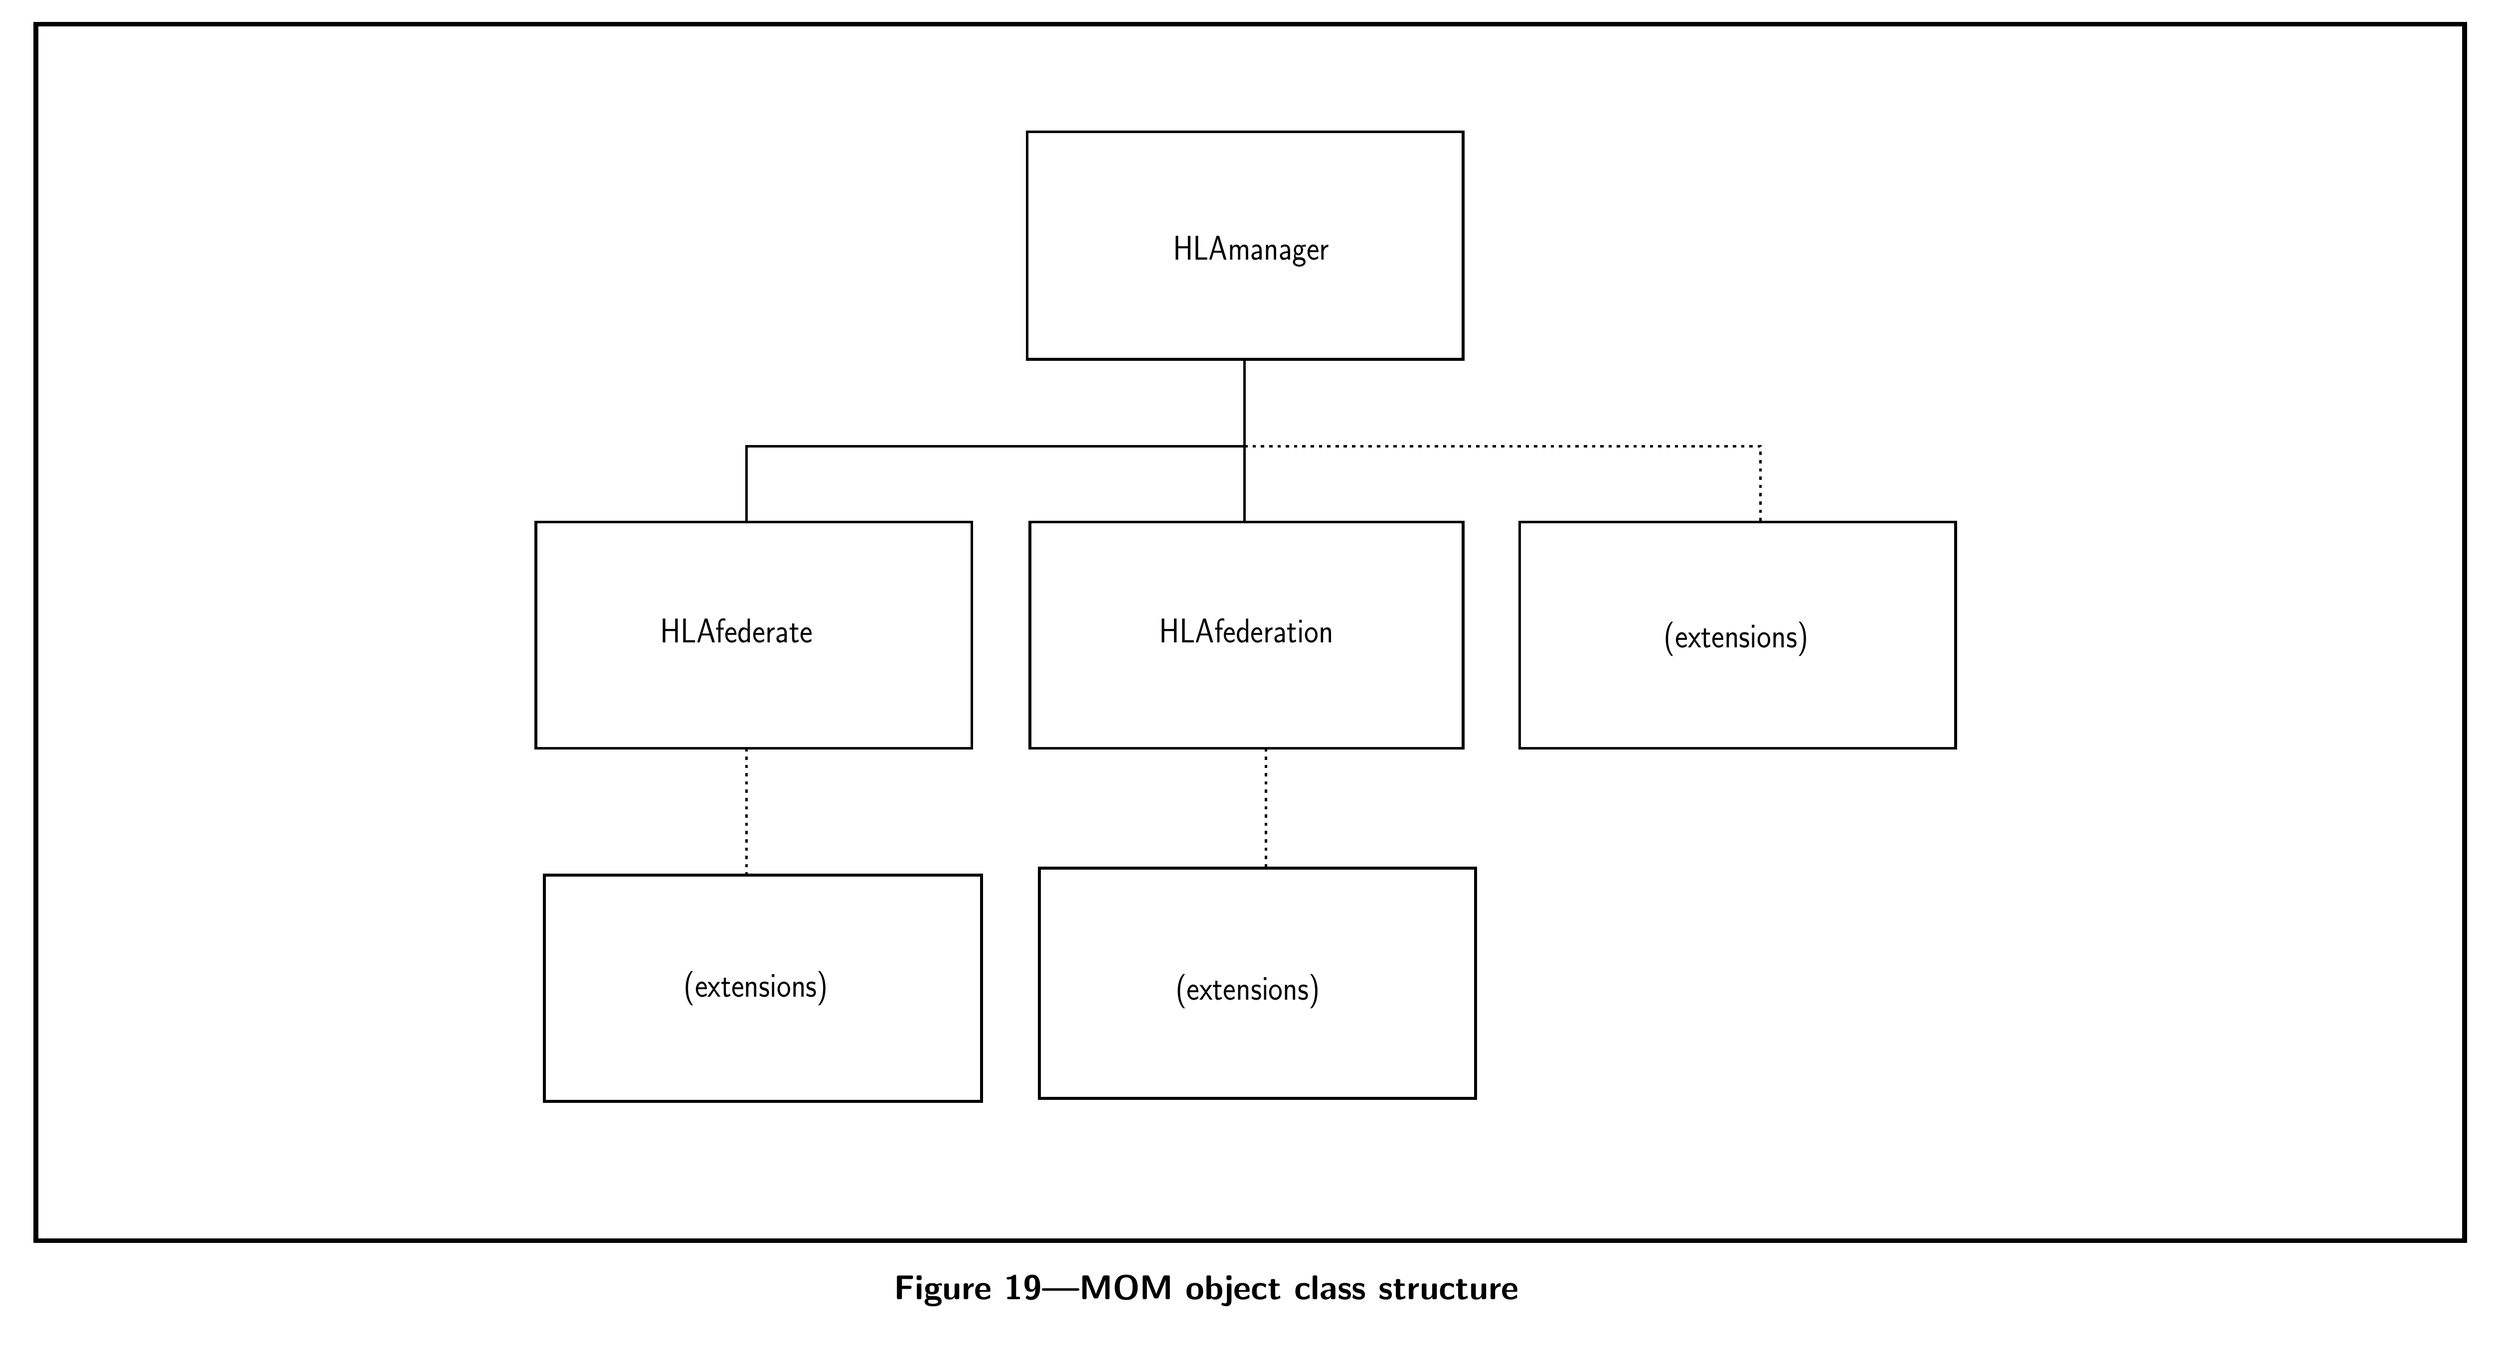
\begin{tikzpicture}[x=1pt,y=-1pt,line cap=butt,line join=miter]
    \path[use as bounding box] (0,0) rectangle (1792,968);

    % Page-local compensation: the reconstruction body text block is slightly left of the source page.
    % A 5-source-pixel shift aligns the native figure frame with source physical page 262.
    \begin{scope}[xshift=5pt]

        % Printed source figure frame.
        \draw[line width=3.4pt] (11,7.5) rectangle (1771.5,889.5);

        % Predefined MOM object-class boxes.
        \draw[line width=2.0pt] (729.5,85.5) rectangle (1045.5,250.5);
        \draw[line width=2.0pt] (373.5,368.5) rectangle (689.5,532.5);
        \draw[line width=2.0pt] (731.5,368.5) rectangle (1045.5,532.5);

        % Extension placeholder boxes.
        \draw[line width=2.0pt] (1086.5,368.5) rectangle (1402.5,532.5);
        \draw[line width=2.0pt] (379.5,624.5) rectangle (696.5,788.5);
        \draw[line width=2.0pt] (738.5,619.5) rectangle (1054.5,786.5);

        % F19-R01: HLAmanager -> HLAfederate, solid predefined hierarchy.
        \draw[line width=1.75pt] (887,250.5) -- (887,313.5) -- (526,313.5) -- (526,368.5);
        % F19-R02: HLAmanager -> HLAfederation, solid predefined hierarchy.
        \draw[line width=1.75pt] (887,313.5) -- (887,368.5);

        % F19-R03: HLAmanager -> direct extension placeholder.
        \draw[line width=1.75pt,dash pattern=on 2.4pt off 3.6pt]
        (887,313.5) -- (1261,313.5) -- (1261,368.5);
        % F19-R04: HLAfederate -> extension placeholder.
        \draw[line width=1.75pt,dash pattern=on 2.4pt off 3.6pt]
        (526,532.5) -- (526,624.5);
        % F19-R05: HLAfederation -> extension placeholder.
        \draw[line width=1.75pt,dash pattern=on 2.4pt off 3.6pt]
        (902.5,532.5) -- (902.5,619.5);

        % Class labels. The exact source raster font is unavailable; Helvetica-family
        % text is horizontally condensed to match the source label widths at page scale.
        \node[font=\sffamily\fontsize{58}{58}\selectfont] at (892.0,172.2)
            {\scalebox{.885}[1]{HLAmanager}};
        \node[font=\sffamily\fontsize{58}{58}\selectfont] at (518.8,447.5)
            {\scalebox{.90}[1]{HLAfederate}};
        \node[font=\sffamily\fontsize{58}{58}\selectfont] at (888.5,447.5)
            {\scalebox{.89}[1]{HLAfederation}};
        \node[font=\sffamily\fontsize{58}{58}\selectfont] at (1243.5,453.5)
            {\scalebox{.891}[1]{(extensions)}};
        \node[font=\sffamily\fontsize{58}{58}\selectfont] at (533.0,706.5)
            {\scalebox{.891}[1]{(extensions)}};
        \node[font=\sffamily\fontsize{58}{58}\selectfont] at (889.5,709.0)
            {\scalebox{.891}[1]{(extensions)}};

        % Native caption, located from the source raster.
        \node[font=\sffamily\bfseries\fontsize{45}{48}\selectfont] at (859.5,926.0)
            {\scalebox{.995}[1]{Figure 19---MOM object class structure}};
    \end{scope}
\end{tikzpicture}
}
    \end{center}
    \vspace{-2pt}
    \vspace{-2pt}

    \subsubsection{Extension of MOM object classes}

    The MOM object classes may be extended by adding subclasses or class attributes. The RTI shall publish HLAmanager.HLAfederate and HLAmanager.HLAfederation classes with predefined MOM class attributes, register an instance, and update the values of the predefined instance attributes.

    The RTI shall not subscribe to any object class. Valid methods for extending the MOM object classes shall be as follows:

    \stdliteralitem{a)}{Subclasses may be added to any MOM object class. Here, the joined federate may publish the object class and its attributes, register an instance of the new class, and update values of instance attributes of the object instance according to the dictates of the federation execution. Note that the instance of the subclass shall be separate from the MOM object instance that is registered by the RTI. Therefore, instance attributes that are inherited by the extension subclass from the MOM predefined class shall not be updated by the RTI.}
    \stdliteralitem{b)}{Attributes may be added to any MOM object class. Here, the joined federate may publish the object class with the new class attributes, may subscribe to the object class and attributes in it, may discover and reflect updates to learn the object instance in question, and may update the values of the new instance attributes (after acquiring ownership) using the discovered object instance designator. Note that the instance that the joined federate shall update with the new instance attributes shall be the same as the MOM object instance that is registered by the RTI. The RTI shall never acquire ownership of any new class attributes.}

    The RTI shall not divest ownership of MOM instance attributes that are defined in this clause. The RTI shall respond to the invocation, by any federate, of the \emph{Request Attribute Value Update} service for any MOM object class or instance attribute that is defined in this clause by supplying values via the normal instance attribute update mechanism.

    \subsection{MOM interaction classes}

    The high-level MOM interaction class structure is depicted in Figure 20. The MOM interaction classes shall be defined as follows:
\end{compactstdpage}

\clearpage

% --- Standard page 249 / source PDF page 263 ---
\begin{compactstdpage}
    \stdliteralitem{a)}{Interaction classes that are subclasses of HLAmanager.\allowbreak{}HLAfederate.\allowbreak{}HLAadjust and HLAmanager.\allowbreak{}Hlafederation.\allowbreak{}HLAadjust shall be acted on by the RTI. They permit a managing federate to adjust how the RTI performs when responding to another federate and how it shall respond and report to the managing federate.}
    \stdliteralitem{b)}{Interaction classes that are subclasses of HLAmanager.\allowbreak{}HLAfederate.\allowbreak{}HLArequest shall be acted on by the RTI. They shall cause the RTI to send subclasses of HLAmanager.\allowbreak{}HLAfederate.\allowbreak{}HLAreport interaction class.}
    \stdliteralitem{c)}{Interaction classes that are subclasses of HLAmanager.\allowbreak{}HLAfederate.\allowbreak{}HLAreport shall be sent by the RTI. They shall respond to interaction classes that are subclasses of HLAmanager.\allowbreak{}HLAfederate.\allowbreak{}HLArequest class interactions. They shall describe some aspect of the federate, such as its object class subscription tree.}
    \stdliteralitem{d)}{Interaction classes that are subclasses of HLAmanager.\allowbreak{}HLAfederate.\allowbreak{}HLAservice shall be acted on by the RTI. They shall invoke HLA services on behalf of another federate. These interactions shall cause the RTI to react as if the service was invoked by that other federate (for example, a managing federate could change the time-regulating state of another federate).}

    \begin{center}
        \resizebox{.66\linewidth}{!}{% Figure 20 - MOM interaction class structure
% Independently reconstructed from IEEE Std 1516.1-2010 source physical p.263 / standard p.249.
% Diagram geometry uses the embedded source stencil's natural 960 x 720 coordinate system.
% Relationship IDs correspond to audit/figure20/relationships.csv.
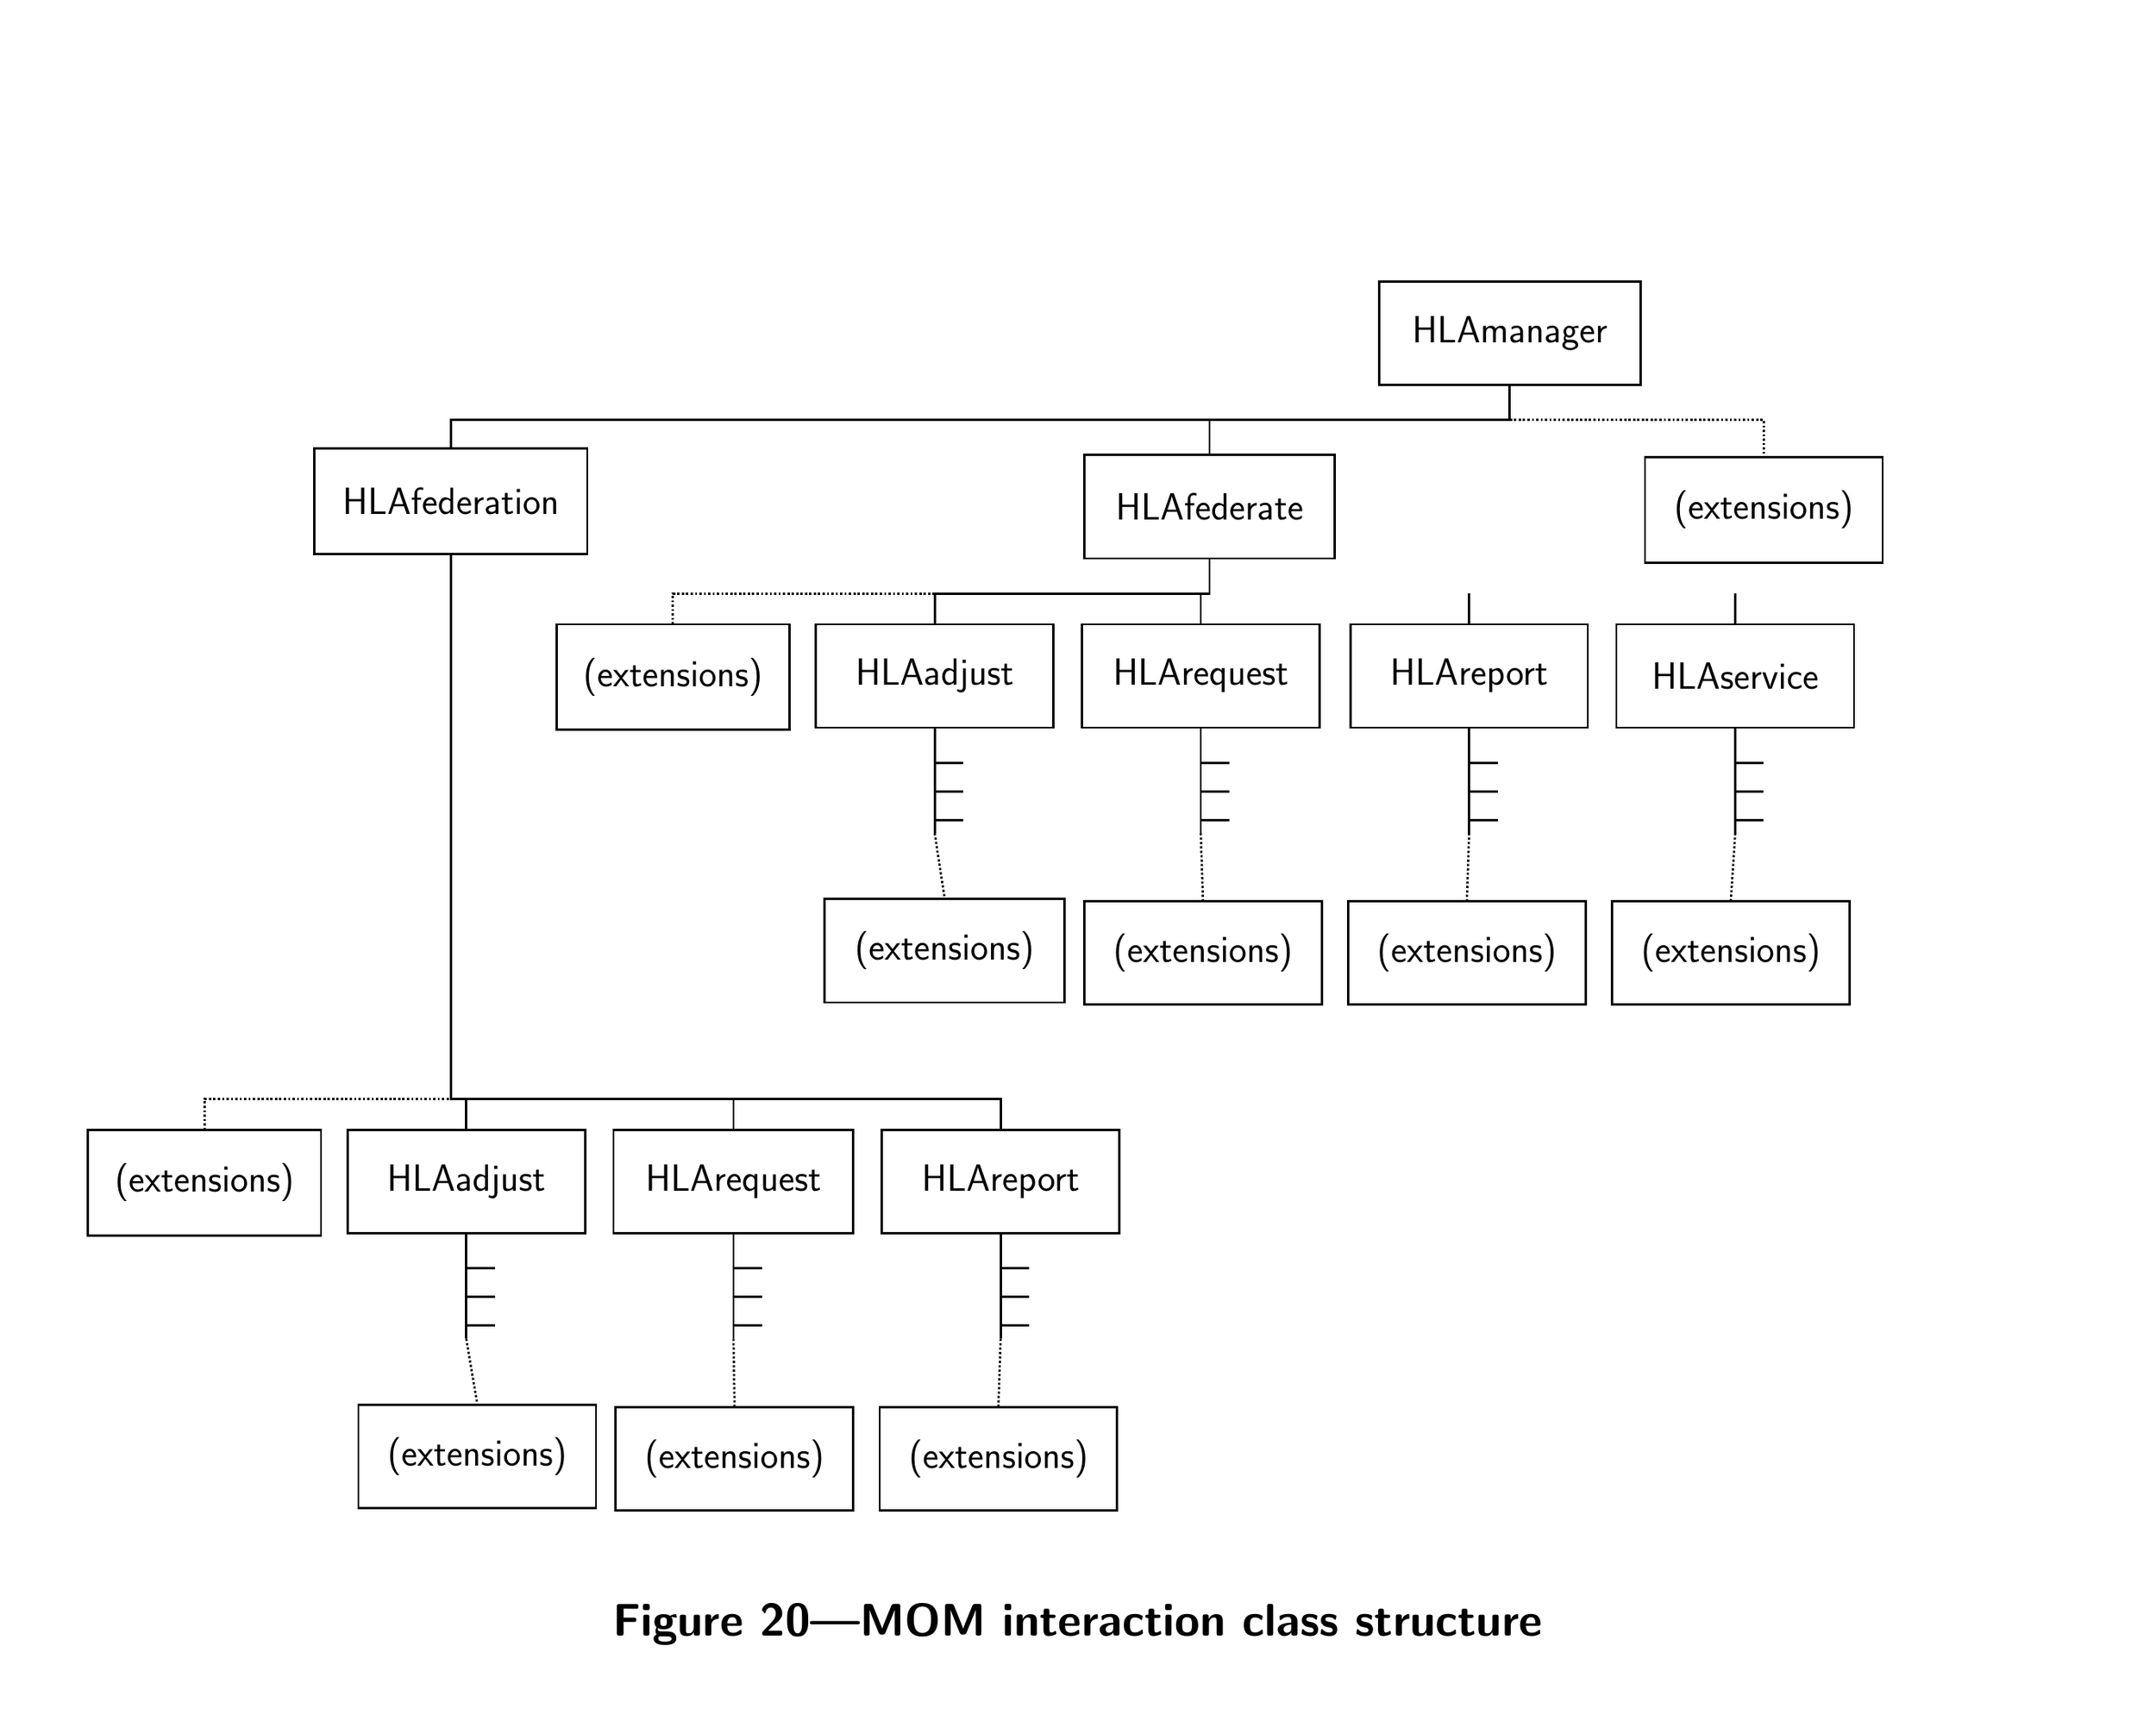
\begin{tikzpicture}[x=1pt,y=-1pt,line cap=butt,line join=miter]
    \path[use as bounding box] (0,0) rectangle (960,760);
    \tikzset{
        fbox/.style={draw,line width=1pt,inner sep=0pt,font=\sffamily\fontsize{17}{17}\selectfont,align=center},
        solid/.style={line width=1pt},
        dotted/.style={densely dotted,line width=1pt}
    }
    % Source-measured predefined and extension boxes.
    \node[fbox,minimum width=119pt,minimum height=47pt] (manager) at (676.5,141.5) {HLAmanager};
    \node[fbox,minimum width=124pt,minimum height=48pt] (federation) at (195,218) {HLAfederation};
    \node[fbox,minimum width=114pt,minimum height=47pt] (federate) at (540,220.5) {HLAfederate};
    \node[fbox,minimum width=108pt,minimum height=48pt] (mgrExt) at (792,222) {(extensions)};

    \node[fbox,minimum width=106pt,minimum height=48pt] (fedExt) at (296,298) {(extensions)};
    \node[fbox,minimum width=108pt,minimum height=47pt] (fAdj) at (415,297.5) {HLAadjust};
    \node[fbox,minimum width=108pt,minimum height=47pt] (fReq) at (536,297.5) {HLArequest};
    \node[fbox,minimum width=108pt,minimum height=47pt] (fRep) at (658,297.5) {HLAreport};
    \node[fbox,minimum width=108pt,minimum height=47pt] (fSvc) at (779,297.5) {HLAservice};

    \node[fbox,minimum width=109pt,minimum height=47pt] (fAdjExt) at (419.5,422.5) {(extensions)};
    \node[fbox,minimum width=108pt,minimum height=47pt] (fReqExt) at (537,423.5) {(extensions)};
    \node[fbox,minimum width=108pt,minimum height=47pt] (fRepExt) at (657,423.5) {(extensions)};
    \node[fbox,minimum width=108pt,minimum height=47pt] (fSvcExt) at (777,423.5) {(extensions)};

    \node[fbox,minimum width=106pt,minimum height=48pt] (gExt) at (83,528) {(extensions)};
    \node[fbox,minimum width=108pt,minimum height=47pt] (gAdj) at (202,527.5) {HLAadjust};
    \node[fbox,minimum width=109pt,minimum height=47pt] (gReq) at (323.5,527.5) {HLArequest};
    \node[fbox,minimum width=108pt,minimum height=47pt] (gRep) at (445,527.5) {HLAreport};
    \node[fbox,minimum width=108pt,minimum height=47pt] (gAdjExt) at (207,652.5) {(extensions)};
    \node[fbox,minimum width=108pt,minimum height=47pt] (gReqExt) at (324,653.5) {(extensions)};
    \node[fbox,minimum width=108pt,minimum height=47pt] (gRepExt) at (444,653.5) {(extensions)};

    % F20-R01..R03: manager-level predefined hierarchy and extension.
    \draw[solid] (676.5,165) -- (676.5,181) -- (195,181) -- (195,194); % F20-R01
    \draw[solid] (540,181) -- (540,197); % F20-R02
    \draw[dotted] (676.5,181) -- (792,181) -- (792,198); % F20-R03

    % F20-R04..R08: HLAfederate family.
    \draw[solid] (540,244) -- (540,260) -- (415,260) -- (415,274); % F20-R04
    \draw[solid] (536,260) -- (536,274); % F20-R05
    \draw[solid] (658,260) -- (658,274); % F20-R06
    \draw[solid] (779,260) -- (779,274); % F20-R07
    \draw[dotted] (415,260) -- (296,260) -- (296,274); % F20-R08

    % F20-R09..R12: omitted predefined subclasses then dotted extensions.
    \foreach \x/\ext in {415/fAdjExt,536/fReqExt,658/fRepExt,779/fSvcExt}{
        \draw[solid] (\x,321) -- (\x,369);
        \draw[solid] (\x,337) -- +(13,0);
        \draw[solid] (\x,350) -- +(13,0);
        \draw[solid] (\x,363) -- +(13,0);
        \draw[dotted] (\x,369) -- (\ext.north);
    }

    % F20-R13..R16: long HLAfederation family trunk and branch.
    \draw[solid] (195,242) -- (195,490) -- (202,490) -- (202,504); % F20-R13
    \draw[solid] (202,490) -- (323.5,490) -- (323.5,504); % F20-R14
    \draw[solid] (323.5,490) -- (445,490) -- (445,504); % F20-R15
    \draw[dotted] (202,490) -- (83,490) -- (83,504); % F20-R16

    % F20-R17..R19: lower omitted-subclass stems and extensions.
    \foreach \x/\ext in {202/gAdjExt,323.5/gReqExt,445/gRepExt}{
        \draw[solid] (\x,551) -- (\x,599);
        \draw[solid] (\x,567) -- +(13,0);
        \draw[solid] (\x,580) -- +(13,0);
        \draw[solid] (\x,593) -- +(13,0);
        \draw[dotted] (\x,599) -- (\ext.north);
    }

    \node[font=\sffamily\bfseries\fontsize{22}{24}\selectfont] at (480,729)
        {Figure 20---MOM interaction class structure};
\end{tikzpicture}
}
    \end{center}
    \vspace{-2pt}
    \vspace{-2pt}

    \subsubsection{Extension of MOM interaction classes}

    The MOM interaction classes may be extended by adding subclasses or parameters. There are three categories of extension of MOM interaction classes as follows:

    \stdliteralitem{a)}{Classes of interaction that the RTI shall send (subclasses of HLAmanager.\allowbreak{}HLAfederate.\allowbreak{}HLAreport). The RTI shall publish at the MOM leaf-class level (e.g., HLAmanager.\allowbreak{}HLAfederate.\allowbreak{}HLAreport.\allowbreak{}HLAreportException). It shall send interactions containing all predefined parameters for that interaction class. Valid methods for extending this type of MOM interaction class are as follows:}
    \stdliteralsubitem{1)}{Subclasses may be added to these MOM interaction classes. The RTI shall not send interactions of these subclasses. If joined federates subscribe to the subclass, they shall receive the full interaction. If they subscribe to the class of which the extension is a subclass, the interaction shall be promoted to the subscribed class, and any new parameters shall be lost.}
    \stdliteralsubitem{2)}{Parameters may be added to any MOM interaction class. Interactions of these classes that are sent by the RTI shall not contain the new parameters.}
\end{compactstdpage}

\clearpage

% --- Standard page 250 / source PDF page 264 ---
\begin{compactstdpage}
    \stdliteralitem{b)}{Classes of interaction that the RTI shall receive (subclasses of HLAmanager.\allowbreak{}HLAfederate.\allowbreak{}HLAadjust, HLAmanager.\allowbreak{}HLAfederate.\allowbreak{}HLArequest, HLAmanager.\allowbreak{}HLAfederate.\allowbreak{}HLAservice, and HLAmanager.\allowbreak{}HLAfederation.\allowbreak{}HLAadjust). The RTI shall subscribe at the MOM leaf-class level (e.g., HLAmanager.\allowbreak{}HLAfederate.\allowbreak{}HLAadjust.\allowbreak{}HLAsetTiming). It shall receive these interactions and process all predefined parameters for that interaction class (with exceptions as listed in the MOM Parameters Definition Table). Valid methods for extending this type of MOM interaction class are as follows:}
    \stdliteralsubitem{1)}{Subclasses may be added to any MOM interaction class. If a joined federate sends an interaction of this class, the RTI shall receive a promoted version that shall contain only the parameters of the predefined interaction class.}
    \stdliteralsubitem{2)}{Parameters may be added to any MOM interaction class. If a joined federate sends an interaction with extra parameters, the RTI shall receive the new parameters, but shall ignore them and process only the predefined parameters.}
    \stdliteralitem{c)}{Classes of interaction that shall be neither sent nor received by the RTI. These classes of interaction shall be ignored by the RTI and may be formed in any way that is consistent with IEEE 1516.2 federation object model (FOM) development.}

    \subsection{MOM-related characteristics of the RTI}

    \subsubsection{Normal RTI MOM administration}

    The RTI deals with MOM object classes and interaction classes in the following ways:

    \stdliteralitem{a)}{The RTI shall publish all leaf object classes in Table 4 that are designated with a ``P.''}
    \stdliteralitem{b)}{For each leaf object class in Table 4, the RTI shall publish all attributes in Table 6 for that object class that are designated with a ``P,'' and no more.}
    \stdliteralitem{c)}{The RTI shall publish all leaf interaction classes in Table 5 that are designated with a ``P.''}
    \stdliteralitem{d)}{In response to an interaction of class HLAmanager.\allowbreak{}HLAfederate.\allowbreak{}HLArequest where the requested information does not exist at the designated federate, the RTI shall send the corresponding interaction of class HLAmanager.\allowbreak{}HLAfederate.\allowbreak{}HLAreport with the appropriate values that indicate a NULL response. The conditions for a NULL response are given in Table 15. The appropriate value and inclusion of a parameter in a NULL response is given in Table 17.}
    \stdliteralsubitem{1)}{The RTI may be required to provide an attribute or parameter whose value is undefined. For an attribute or parameter having an array value, an undefined value shall be encoded as an empty (zero-length) array.}
    \stdliteralitem{e)}{When sending an interaction of one of the leaf classes in Table 5 that is not a NULL response, the RTI shall always supply all parameters listed in Table 7 for that interaction class, and no more.}
    \stdliteralitem{f)}{The RTI shall be actively subscribed to all leaf interaction classes in Table 5 that are designated with an ``S.''}
    \stdliteralitem{g)}{The RTI shall be neither time-regulating nor time-constrained and shall never provide timestamps or user-supplied tags with instance attribute updates, sent interactions, or deletion of object instances.}
    \stdliteralitem{h)}{The RTI shall update the values of all attributes of instances of HLAmanager.HLAfederate found in Table 6 using an update region set that contains a single region. The region used with each instance attribute shall contain only the HLAfederate dimension as a specified dimension. The range for that dimension shall be a point range around the normalized value (using the Normalize Federate Handle service) of the HLAfederateHandle attribute of that object instance.}
\end{compactstdpage}

\clearpage

% --- Standard page 251 / source PDF page 265 ---
\begin{compactstdpage}
    \stdliteralitem{i)}{The RTI shall send all interactions of class HLAmanager.\allowbreak{}HLAfederate.\allowbreak{}HLAreport.\allowbreak{}HLAreportServiceInvocation using an update region set that contains a single region. The region used with each such interaction shall contain only the HLAfederate and HLAserviceGroup dimensions as specified dimensions. The range used for the HLAfederate dimension shall be a point range around the normalized value (using the Normalize Federate Handle service) of the HLAfederate parameter of that interaction. The range used for the HLAserviceGroup dimension shall be a point range around the normalized value (using the Normalize Service Group service) of the service group in which the service indicated in the HLAservice parameter is found.}
    \stdliteralitem{j)}{The RTI shall send all other interactions that are of subclasses of HLAmanager.\allowbreak{}HLAfederate.\allowbreak{}HLAreport in Table 5 using an update region set that contains a single region. The region used with each such interaction shall contain only the HLAfederate dimension as a specified dimension. The range for that dimension shall be a point range around the normalized value (using the Normalize Federate Handle service) of the HLAfederate parameter of that interaction.}
    \stdliteralitem{k)}{Other than registering and deleting object instances, updating instance attributes, and sending and receiving interactions, the RTI shall not engage in any other activity with regard to MOM. In other words, among other things, an RTI shall never}
    \stdliteralsubitem{1)}{Engage in ownership transfer of MOM instance attributes.}
    \stdliteralsubitem{2)}{Modify the transportation or order type of a MOM instance attribute or interaction class.}
    \stdliteralsubitem{3)}{Use DDM services with MOM instance attributes or interaction classes, except as noted above.}
    \stdliteralitem{l)}{Unless specifically noted otherwise in Table 17, when a federate sends an interaction, it shall always supply all pre-defined parameters that are available at that interaction class and no more, with the following exceptions:}
    \stdliteralsubitem{1)}{A federate shall not be required to supply parameters of any HLAmanager.\allowbreak{}HLAfederate.\allowbreak{}HLAservice interaction that correspond to optional arguments of the HLA service that the HLAmanager.\allowbreak{}HLAfederate.\allowbreak{}HLAservice interaction is intended to cause to be invoked on behalf of another federate. (For example, HLAattributeList is not a required parameter of the HLAmanager.\allowbreak{}HLAfederate.\allowbreak{}HLAservice.HLAunpublishObjectClassAttributes interaction because the set of attribute designators argument of the Unpublish Object Class Attributes service is an optional argument to that service.)}
    \stdliteralsubitem{2)}{A federate shall supply at least one of the parameters of the HLAmanager.\allowbreak{}HLAfederate.\allowbreak{}HLAadjust.\allowbreak{}HLAsetSwitches interaction.}

    \subsubsection{Sending MOM interactions by federates during federate save/restore}

    Although sending interactions is normally forbidden while federate saves and restores are in progress, the following deviations to this rule shall be allowed (assuming the correct publications are in place):

    \stdliteralitem{a)}{A joined federate shall be allowed to send either a MOM HLAfederateSaveBegun or a MOM HLAfederateSaveComplete interaction when a federate save is in progress.}
    \stdliteralitem{b)}{A joined federate shall be allowed to send a MOM HLAfederateRestoreComplete interaction when a federate restore is in progress.}
\end{compactstdpage}

\clearpage

% --- Standard page 252 / source PDF page 266 ---
\begin{compactstdpage}
    \subsection{Service reporting}

    The HLAmanager.\allowbreak{}HLAfederate.\allowbreak{}HLAreport.\allowbreak{}HLAreportServiceInvocation interaction shall be sent by the RTI whenever an HLA service is invoked, either by a particular joined federate or by the RTI at a particular joined federate, and service reporting switch is enabled for that particular joined federate. The service reporting switch value for a specific joined federate shall be determined in the following manner:

    \stdliteralitem{a)}{The initial value for the service reporting switch for that joined federate shall be the value of the service reporting switch in the federation execution's FDD (enabled or disabled).}
    \stdliteralitem{b)}{If one or more HLAmanager.\allowbreak{}HLAfederate.\allowbreak{}HLAadjust.\allowbreak{}HLAsetSwitches interactions have set the service reporting switch for that joined federate, the value shall be that set by the last interaction (enabled or disabled).}

    If a joined federate is subscribed to the HLAmanager.\allowbreak{}HLAfederate.\allowbreak{}HLAreport.\allowbreak{}HLAreportServiceInvocation interaction, all attempts to set the service reporting switch for that joined federate to enabled by sending an HLAmanager.\allowbreak{}HLAfederate.\allowbreak{}HLAadjust.\allowbreak{}HLAsetSwitches interaction shall fail and be reported via the normal MOM interaction failure means. If a joined federate has the Service Reporting Switch Enabled, that joined federate shall not be able to subscribe to the HLAmanager.\allowbreak{}HLAfederate.\allowbreak{}HLAreport.\allowbreak{}HLAreportServiceInvocation interaction class.

    \subsection{MOM OMT tables}

    The elements that constitute MOM are depicted in OMT format (found in IEEE Std 1516.2-2010) in Table 4 through Table 17. The MOM table information in this clause shall appear in all compliant FOMs (see IEEE Std 1516-2010 and IEEE Std 1516.2-2010) and shall not be altered. Note that MOM does not use many of the OMT tables (e.g., time representation table, user-supplied tag table, synchronization table, transportation type table, switches table, and variant record table). They have been omitted from the depiction.

    If there are any differences between the MOM tables defined in this clause (i.e., Clause 11) and the tables defined in the MOM and Initialization Module (MIM) in Annex G, this clause shall take precedence.

    \momtabletitle{Table 4---MOM object class structure table}
    \begin{momtabletypeset}[7.0]
        \begin{center}
            \begin{tabular}{Y{1.75in}Y{1.75in}Y{1.45in}}
                HLAobjectRoot (N) & HLAmanager (N) & HLAfederate (P)   \\
                &                & HLAfederation (P)
            \end{tabular}
        \end{center}
    \end{momtabletypeset}
\end{compactstdpage}

\clearpage
% --- Standard page 253 / source PDF page 267 ---
\begin{compactstdpage}
    \momtabletitle{Table 5---MOM interaction class structure table}
    \begin{momtabletypeset}[8.00]
        \makebox[\linewidth][c]{%
            \resizebox{0.912\linewidth}{!}{%
                \begin{tabular}{|Y{76.87pt}|Y{60.44pt}|Y{67.64pt}|Y{54.56pt}|Y{156.97pt}|}
                    \hline
                    HLAinteractionRoot\newline (N) & HLAmanager (N) & HLAfederate (N) & HLAadjust (N)          & HLAsetTiming (S)                                      \\
                    \cline{5-5}
                    &                &                 &                        & HLAmodifyAttributeState (S)                           \\
                    \cline{5-5}
                    &                &                 &                        & HLAsetSwitches (S)                                    \\
                    \cline{4-5}
                    &                &                 & HLArequest\newline (N) & HLArequestPublications (S)                            \\
                    \cline{5-5}
                    &                &                 &                        & HLArequestSubscriptions (S)                           \\
                    \cline{5-5}
                    &                &                 &                        & HLArequestObjectInstancesThatCanBeDeleted\newline (S) \\
                    \cline{5-5}
                    &                &                 &                        & HLArequestObjectInstancesUpdated (S)                  \\
                    \cline{5-5}
                    &                &                 &                        & HLArequestObjectInstancesReflected (S)                \\
                    \cline{5-5}
                    &                &                 &                        & HLArequestUpdatesSent (S)                             \\
                    \cline{5-5}
                    &                &                 &                        & HLArequestInteractionsSent (S)                        \\
                    \cline{5-5}
                    &                &                 &                        & HLArequestReflectionsReceived (S)                     \\
                    \cline{5-5}
                    &                &                 &                        & HLArequestInteractionsReceived (S)                    \\
                    \cline{5-5}
                    &                &                 &                        & HLArequestObjectInstanceInformation (S)               \\
                    \cline{5-5}
                    &                &                 &                        & HLArequestFOMmoduleData (S)                           \\
                    \cline{4-5}
                    &                &                 & HLAreport (N)          & HLAreportObjectClassPublication (P)                   \\
                    \cline{5-5}
                    &                &                 &                        & HLAreportObjectClassSubscription (P)                  \\
                    \cline{5-5}
                    &                &                 &                        & HLAreportInteractionPublication (P)                   \\
                    \cline{5-5}
                    &                &                 &                        & HLAreportInteractionSubscription (P)                  \\
                    \cline{5-5}
                    &                &                 &                        & HLAreportObjectInstancesThatCanBeDeleted\newline (P)  \\
                    \cline{5-5}
                    &                &                 &                        & HLAreportObjectInstancesUpdated (P)                   \\
                    \cline{5-5}
                    &                &                 &                        & HLAreportObjectInstancesReflected (P)                 \\
                    \cline{5-5}
                    &                &                 &                        & HLAreportUpdatesSent (P)                              \\
                    \cline{5-5}
                    &                &                 &                        & HLAreportReflectionsReceived (P)                      \\
                    \cline{5-5}
                    &                &                 &                        & HLAreportInteractionsSent (P)                         \\
                    \cline{5-5}
                    &                &                 &                        & HLAreportInteractionsReceived (P)                     \\
                    \cline{5-5}
                    &                &                 &                        & HLAreportObjectInstanceInformation (P)                \\
                    \cline{5-5}
                    &                &                 &                        & HLAreportException (P)                                \\
                    \cline{5-5}
                    &                &                 &                        & HLAreportServiceInvocation (P)                        \\
                    \cline{5-5}
                    &                &                 &                        & HLAreportMOMexception (P)                             \\
                    \cline{5-5}
                    &                &                 &                        & HLAreportFederateLost (P)                             \\
                    \cline{5-5}
                    &                &                 &                        & HLAreportFOMmoduleData (P)                            \\
                    \cline{4-5}
                    &                &                 & HLAservice (N)         & HLAresignFederationExecution (S)                      \\
                    \cline{5-5}
                    &                &                 &                        & HLAsynchronizationPointAchieved (S)                   \\
                    \cline{5-5}
                    &                &                 &                        & HLAfederateSaveBegun (S)                              \\
                    \cline{5-5}
                    &                &                 &                        & HLAfederateSaveComplete (S)                           \\
                    \cline{5-5}
                    &                &                 &                        & HLAfederateRestoreComplete (S)                        \\
                    \cline{5-5}
                    &                &                 &                        & HLApublishObjectClassAttributes (S)                   \\
                    \cline{5-5}
                    &                &                 &                        & HLAunpublishObjectClassAttributes (S)                 \\
                    \cline{5-5}
                    &                &                 &                        & HLApublishInteractionClass (S)                        \\
                    \cline{5-5}
                    &                &                 &                        & HLAunpublishInteractionClass (S)                      \\
                    \cline{5-5}
                    &                &                 &                        & HLAsubscribeObjectClassAttributes (S)                 \\
                    \hline
                \end{tabular}%
            }% resizebox
        }% makebox
    \end{momtabletypeset}
\end{compactstdpage}
\clearpage

% --- Standard page 254 / source PDF page 268 ---
\begin{compactstdpage}
    \momtabletitle{Table 5---MOM interaction class structure table \textit{(continued)}}
    \begin{momtabletypeset}[8.00]
        \makebox[\linewidth][c]{%
            \resizebox{0.912\linewidth}{!}{%
                \begin{tabular}{|Y{76.87pt}|Y{60.44pt}|Y{67.64pt}|Y{54.56pt}|Y{156.97pt}|}
                    \hline
                    & &                   &                        & HLAunsubscribeObjectClassAttributes (S)                     \\
                    \cline{5-5}
                    & &                   &                        & HLAsubscribeInteractionClass (S)                            \\
                    \cline{5-5}
                    & &                   &                        & HLAunsubscribeInteractionClass (S)                          \\
                    \cline{5-5}
                    & &                   &                        & HLAdeleteObjectInstance (S)                                 \\
                    \cline{5-5}
                    & &                   &                        & HLAlocalDeleteObjectInstance (S)                            \\
                    \cline{5-5}
                    & &                   &                        & HLArequestAttributeTransportationypeChange\newline (S)      \\
                    \cline{5-5}
                    & &                   &                        & HLArequestInteractionTransportationype-\newline Change (S)  \\
                    \cline{5-5}
                    & &                   &                        & HLAunconditionalAttributeOwnershipDives-\newline titure (S) \\
                    \cline{5-5}
                    & &                   &                        & HLAenableTimeRegulation (S)                                 \\
                    \cline{5-5}
                    & &                   &                        & HLAdisableTimeRegulation (S)                                \\
                    \cline{5-5}
                    & &                   &                        & HLAenableTimeConstrained (S)                                \\
                    \cline{5-5}
                    & &                   &                        & HLAdisableTimeConstrained (S)                               \\
                    \cline{5-5}
                    & &                   &                        & HLAtimeAdvanceRequest (S)                                   \\
                    \cline{5-5}
                    & &                   &                        & HLAtimeAdvanceRequestAvailable (S)                          \\
                    \cline{5-5}
                    & &                   &                        & HLAnextMessageRequest (S)                                   \\
                    \cline{5-5}
                    & &                   &                        & HLAnextMessageRequestAvailable (S)                          \\
                    \cline{5-5}
                    & &                   &                        & HLAflushQueueRequest (S)                                    \\
                    \cline{5-5}
                    & &                   &                        & HLAenableAsynchronousDelivery (S)                           \\
                    \cline{5-5}
                    & &                   &                        & HLAdisableAsynchronousDelivery (S)                          \\
                    \cline{5-5}
                    & &                   &                        & HLAmodifyLookahead (S)                                      \\
                    \cline{5-5}
                    & &                   &                        & HLAchangeAttributeOrderType (S)                             \\
                    \cline{5-5}
                    & &                   &                        & HLAchangeInteractionOrderType (S)                           \\
                    \cline{3-5}
                    & & HLAfederation (N) & HLAadjust (N)          & HLAsetSwitches (S)                                          \\
                    \cline{4-5}
                    & &                   & HLArequest\newline (N) & HLArequestSynchronizationPoints (S)                         \\
                    \cline{5-5}
                    & &                   &                        & HLArequestSynchronizationPointStatus (S)                    \\
                    \cline{5-5}
                    & &                   &                        & HLArequestFOMmoduleData (S)                                 \\
                    \cline{5-5}
                    & &                   &                        & HLArequestMIMData (S)                                       \\
                    \cline{4-5}
                    & &                   & HLAreport (N)          & HLAreportSynchronizationPoints (P)                          \\
                    \cline{5-5}
                    & &                   &                        & HLAreportSynchronizationPointStatus (P)                     \\
                    \cline{5-5}
                    & &                   &                        & HLAreportFOMmoduleData (P)                                  \\
                    \cline{5-5}
                    & &                   &                        & HLAreportMIMData (P)                                        \\
                    \hline
                \end{tabular}%
            }% resizebox
        }% makebox
    \end{momtabletypeset}
\end{compactstdpage}
\clearpage

\begin{landscape}
% --- Standard page 255 / source PDF page 269 ---
    \thispagestyle{body}
    \momtabletitle{Table 6---MOM attribute table}
    \begin{momtabletypeset}[8.00]
        \makebox[\linewidth][c]{%
            \resizebox{0.930\linewidth}{!}{%
                \begin{tabular}{|Y{90.94pt}|Y{96.62pt}|Y{69.32pt}|Y{45.50pt}|Y{96.56pt}|Y{24.62pt}|Y{24.62pt}|Y{48.56pt}|Y{65.24pt}|Y{36.37pt}|}
                    \hline
                    \Centering\arraybackslash\bfseries Object                               & \Centering\arraybackslash\bfseries Attribute & \Centering\arraybackslash\bfseries Datatype & \Centering\arraybackslash\bfseries Update\allowbreak{}type & \Centering\arraybackslash\bfseries Update\allowbreak{}condition & \Centering\arraybackslash\bfseries D/\allowbreak{}A & \Centering\arraybackslash\bfseries P/\allowbreak{}S & \Centering\arraybackslash\bfseries Available\allowbreak{}dimensions & \Centering\arraybackslash\bfseries Transportation & \Centering\arraybackslash\bfseries Order \\
                    \hline
                    HLAobjectRoot.\allowbreak{}\newline HLAmanager.\allowbreak{}HLAfederate & HLAfederateHandle & HLAhandle & Static & NA & N & P & HLAfederate & HLAreliable & Receive \\
                    \cline{2-10}
                    & HLAfederateName                              & HLAunicodeString                            & Static                                                     & NA                                                                                                                                                                                                                                                                                                                  & N                                                   & P                                                   & HLAfederate                                                         & HLAreliable                                       & Receive                                  \\
                    \cline{2-10}
                    & HLAfederateType                              & HLAunicodeString                            & Static                                                     & NA                                                                                                                                                                                                                                                                                                                  & N                                                   & P                                                   & HLAfederate                                                         & HLAreliable                                       & Receive                                  \\
                    \cline{2-10}
                    & HLAfederateHost                              & HLAunicodeString                            & Static                                                     & NA                                                                                                                                                                                                                                                                                                                  & N                                                   & P                                                   & HLAfederate                                                         & HLAreliable                                       & Receive                                  \\
                    \cline{2-10}
                    & HLARTIversion                                & HLAunicodeString                            & Static                                                     & NA                                                                                                                                                                                                                                                                                                                  & N                                                   & P                                                   & HLAfederate                                                         & HLAreliable                                       & Receive                                  \\
                    \cline{2-10}
                    & HLAFOMmoduleDesigna-\newline torList         & HLAmoduleDesig-\newline natorlist           & Static                                                     & N/\allowbreak{}A & N & P & HLAfederate & HLAreliable & Receive \\
                    \cline{2-10}
                    & HLAtimeConstrained                           & HLAboolean                                  & Conditional                                                & Whenever services Time\allowbreak{}Constrained Enabled † or\allowbreak{}Disable Time Constrained\allowbreak{}are successfully invoked\newline (including via the HLA-\newline disableTimeConstrained\allowbreak{}interaction).\allowbreak{} & N & P & HLAfederate & HLAreliable & Receive \\
                    \cline{2-10}
                    & HLAtimeRegulating                            & HLAboolean                                  & Conditional                                                & Whenever services Time\allowbreak{}Regulation Enabled † or\allowbreak{}Disable Time Regulation are\allowbreak{}successfully invoked\newline (including via the\allowbreak{}HLAdisableTimeRegulation\allowbreak{}interaction).\allowbreak{} & N & P & HLAfederate & HLAreliable & Receive \\
                    \cline{2-10}
                    & HLAasynchronousDelivery                      & HLAboolean                                  & Conditional                                                & Whenever services Enable\allowbreak{}Asynchronous Delivery or\allowbreak{}Disable Asynchronous\allowbreak{}Delivery are successfully\allowbreak{}invoked (including via the\allowbreak{}HLAenableAsynchronous-\newline Delivery or HLAdisable-\newline AsynchronousDelivery\allowbreak{}interactions).\allowbreak{} & N & P & HLAfederate & HLAreliable & Receive \\
                    \hline
                \end{tabular}%
            }% resizebox
        }% makebox
    \end{momtabletypeset}
    \newpage

% --- Standard page 256 / source PDF page 270 ---
    \thispagestyle{body}
    \momtabletitle{Table 6---MOM attribute table \textit{(continued)}}
    \begin{momtabletypeset}[8.00]
        \makebox[\linewidth][c]{%
            \resizebox{0.930\linewidth}{!}{%
                \begin{tabular}{|Y{90.88pt}|Y{96.62pt}|Y{69.32pt}|Y{45.50pt}|Y{96.56pt}|Y{24.62pt}|Y{24.62pt}|Y{48.56pt}|Y{65.24pt}|Y{36.31pt}|}
                    \hline
                    \Centering\arraybackslash\bfseries Object & \Centering\arraybackslash\bfseries Attribute & \Centering\arraybackslash\bfseries Datatype & \Centering\arraybackslash\bfseries Update\allowbreak{}type & \Centering\arraybackslash\bfseries Update\allowbreak{}condition & \Centering\arraybackslash\bfseries D/\allowbreak{}A & \Centering\arraybackslash\bfseries P/\allowbreak{}S & \Centering\arraybackslash\bfseries Available\allowbreak{}dimensions & \Centering\arraybackslash\bfseries Transportation & \Centering\arraybackslash\bfseries Order \\
                    \hline
                    & HLAfederateState                             & HLAfederateState                            & Conditional                                                & Whenever the services\allowbreak{}Initiate Federate Save †,\newline Federation Saved †,\newline Federation Restore Begun †,\newline Confirm Federation\allowbreak{}Restoration Request\newline (success) †, or Join\allowbreak{}Federation Execution are\allowbreak{}successfully invoked.\allowbreak{} Also,\newline after the Federation\allowbreak{}Restored † service has been\allowbreak{}invoked at all federates in the\allowbreak{}federation execution.\allowbreak{} If a\allowbreak{}joined federate is in the\allowbreak{}Federate Save in Progress\allowbreak{}state, no corresponding\allowbreak{}reflects shall be invoked at\allowbreak{}that joined federate.\allowbreak{} & N & P & HLAfederate & HLAreliable & Receive \\
                    \cline{2-10}
                    & HLAtimeManagerState                          & HLAtimeState                                & Conditional                                                & Whenever services Time\allowbreak{}Advance Request, Time\allowbreak{}Advance Request Available,\newline Next Message Request, Next\allowbreak{}Message Request Available,\newline Flush Queue Request, or\allowbreak{}Time Advance Grant † are\allowbreak{}successfully invoked\newline (including via the\allowbreak{}HLAtimeAdvanceRequest,\newline HLAtimeAdvanceRequest-\newline Available, HLAnext-\newline MessageRequest,\newline HLAnextMessageRequest-\newline Available, or HLAflush-\newline QueueRequest interactions).\allowbreak{} & N & P & HLAfederate & HLAreliable & Receive \\
                    \cline{2-10}
                    & HLAlogicalTime                               & HLAlogicalTime                              & Periodic                                                   & HLAsetTiming.\allowbreak{}\newline HLAreportPeriod & N & P & HLAfederate & HLAreliable & Receive \\
                    \cline{2-10}
                    & HLAlookahead                                 & HLAtimeInterval                             & Periodic                                                   & HLAsetTiming.\allowbreak{}\newline HLAreportPeriod & N & P & HLAfederate & HLAreliable & Receive \\
                    \cline{2-10}
                    & HLAGALT                                      & HLAlogicalTime                              & Periodic                                                   & HLAsetTiming.\allowbreak{}\newline HLAreportPeriod & N & P & HLAfederate & HLAreliable & Receive \\
                    \hline
                \end{tabular}%
            }% resizebox
        }% makebox
    \end{momtabletypeset}
    \newpage

% --- Standard page 257 / source PDF page 271 ---
    \thispagestyle{body}
    \momtabletitle{Table 6---MOM attribute table \textit{(continued)}}
    \begin{momtabletypeset}[8.00]
        \makebox[\linewidth][c]{%
            \resizebox{0.930\linewidth}{!}{%
                \begin{tabular}{|Y{90.88pt}|Y{96.62pt}|Y{69.32pt}|Y{45.50pt}|Y{96.56pt}|Y{24.62pt}|Y{24.62pt}|Y{48.56pt}|Y{65.24pt}|Y{36.31pt}|}
                    \hline
                    \Centering\arraybackslash\bfseries Object & \Centering\arraybackslash\bfseries Attribute & \Centering\arraybackslash\bfseries Datatype & \Centering\arraybackslash\bfseries Update\allowbreak{}type & \Centering\arraybackslash\bfseries Update\allowbreak{}condition & \Centering\arraybackslash\bfseries D/\allowbreak{}A & \Centering\arraybackslash\bfseries P/\allowbreak{}S & \Centering\arraybackslash\bfseries Available\allowbreak{}dimensions & \Centering\arraybackslash\bfseries Transportation & \Centering\arraybackslash\bfseries Order \\
                    \hline
                    & HLALITS                                      & HLAlogicalTime                              & Periodic                                                   & HLAsetTiming.\allowbreak{}\newline HLAreportPeriod & N & P & HLAfederate & HLAreliable & Receive \\
                    \cline{2-10}
                    & HLAROlength                                  & HLAcount                                    & Periodic                                                   & HLAsetTiming.\allowbreak{}\newline HLAreportPeriod & N & P & HLAfederate & HLAreliable & Receive \\
                    \cline{2-10}
                    & HLATSOlength                                 & HLAcount                                    & Periodic                                                   & HLAsetTiming.\allowbreak{}\newline HLAreportPeriod & N & P & HLAfederate & HLAreliable & Receive \\
                    \cline{2-10}
                    & HLAreflectionsReceived                       & HLAcount                                    & Periodic                                                   & HLAsetTiming.\allowbreak{}\newline HLAreportPeriod & N & P & HLAfederate & HLAreliable & Receive \\
                    \cline{2-10}
                    & HLAupdatesSent                               & HLAcount                                    & Periodic                                                   & HLAsetTiming.\allowbreak{}\newline HLAreportPeriod & N & P & HLAfederate & HLAreliable & Receive \\
                    \cline{2-10}
                    & HLAinteractionsReceived                      & HLAcount                                    & Periodic                                                   & HLAsetTiming.\allowbreak{}\newline HLAreportPeriod & N & P & HLAfederate & HLAreliable & Receive \\
                    \cline{2-10}
                    & HLAinteractionsSent                          & HLAcount                                    & Periodic                                                   & HLAsetTiming.\allowbreak{}\newline HLAreportPeriod & N & P & HLAfederate & HLAreliable & Receive \\
                    \cline{2-10}
                    & HLAobjectInstancesThat-\newline CanBeDeleted & HLAcount                                    & Periodic                                                   & HLAsetTiming.\allowbreak{}\newline HLAreportPeriod & N & P & HLAfederate & HLAreliable & Receive \\
                    \cline{2-10}
                    & HLAobjectInstancesUpdated                    & HLAcount                                    & Periodic                                                   & HLAsetTiming.\allowbreak{}\newline HLAreportPeriod & N & P & HLAfederate & HLAreliable & Receive \\
                    \cline{2-10}
                    & HLAobjectInstances-\newline Reflected        & HLAcount                                    & Periodic                                                   & HLAsetTiming.\allowbreak{}\newline HLAreportPeriod & N & P & HLAfederate & HLAreliable & Receive \\
                    \cline{2-10}
                    & HLAobjectInstancesDeleted                    & HLAcount                                    & Periodic                                                   & HLAsetTiming.\allowbreak{}\newline HLAreportPeriod & N & P & HLAfederate & HLAreliable & Receive \\
                    \cline{2-10}
                    & HLAobjectInstances-\newline Removed          & HLAcount                                    & Periodic                                                   & HLAsetTiming.\allowbreak{}\newline HLAreportPeriod & N & P & HLAfederate & HLAreliable & Receive \\
                    \cline{2-10}
                    & HLAobjectInstances-\newline Registered       & HLAcount                                    & Periodic                                                   & HLAsetTiming.\allowbreak{}\newline HLAreportPeriod & N & P & HLAfederate & HLAreliable & Receive \\
                    \cline{2-10}
                    & HLAobjectInstances-\newline Discovered       & HLAcount                                    & Periodic                                                   & HLAsetTiming.\allowbreak{}\newline HLAreportPeriod & N & P & HLAfederate & HLAreliable & Receive \\
                    \cline{2-10}
                    & HLAtimeGrantedTime                           & HLAmsec                                     & Periodic                                                   & HLAsetTiming.\allowbreak{}\newline HLAreportPeriod & N & P & HLAfederate & HLAreliable & Receive \\
                    \cline{2-10}
                    & HLAtimeAdvancingTime                         & HLAmsec                                     & Periodic                                                   & HLAsetTiming.\allowbreak{}\newline HLAreportPeriod & N & P & HLAfederate & HLAreliable & Receive \\
                    \hline
                \end{tabular}%
            }% resizebox
        }% makebox
    \end{momtabletypeset}
    \newpage

% --- Standard page 258 / source PDF page 272 ---
    \thispagestyle{body}
    \momtabletitle{Table 6---MOM attribute table \textit{(continued)}}
    \begin{momtabletypeset}[8.00]
        \makebox[\linewidth][c]{%
            \resizebox{0.930\linewidth}{!}{%
                \begin{tabular}{|Y{90.88pt}|Y{96.62pt}|Y{69.32pt}|Y{45.50pt}|Y{96.56pt}|Y{24.62pt}|Y{24.62pt}|Y{48.56pt}|Y{65.24pt}|Y{36.31pt}|}
                    \hline
                    \Centering\arraybackslash\bfseries Object       & \Centering\arraybackslash\bfseries Attribute & \Centering\arraybackslash\bfseries Datatype & \Centering\arraybackslash\bfseries Update\allowbreak{}type & \Centering\arraybackslash\bfseries Update\allowbreak{}condition & \Centering\arraybackslash\bfseries D/\allowbreak{}A & \Centering\arraybackslash\bfseries P/\allowbreak{}S & \Centering\arraybackslash\bfseries Available\allowbreak{}dimensions & \Centering\arraybackslash\bfseries Transportation & \Centering\arraybackslash\bfseries Order \\
                    \hline
                    & HLAconveyRegionDesignat\allowbreak{}orSets   & HLAswitch                                   & Conditional                                                & Whenever the\allowbreak{}HLAmanager.\allowbreak{}HLAfederate.\allowbreak{}\newline HLAfederate.\allowbreak{}HLA-\newline adjust.\allowbreak{}HLAsetSwitches\allowbreak{}interaction is sent to\allowbreak{}successfully change the\allowbreak{}value of the HLAconvey-\newline RegionDesignatorSets\allowbreak{}parameter.\allowbreak{} & N & P & HLAfederate & HLAreliable & Receive \\
                    \cline{2-10}
                    & HLAconveyProducing-\newline Federate         & HLAswitch                                   & Conditional                                                & Whenever the\allowbreak{}HLAmanager.\allowbreak{}HLAfederate.\allowbreak{}\newline HLAadjust.\allowbreak{}HLAsetSwitches\allowbreak{}interaction is sent to\allowbreak{}successfully change the\allowbreak{}value of the\allowbreak{}HLAconveyProducing-\newline Federate parameter.\allowbreak{} & N & P & HLAfederate & HLAreliable & Receive \\
                    \hline
                    HLAmanager.\allowbreak{}HLAfedera-\newline tion & HLAfederationName                            & HLAunicodeString & Static & NA & N & P & NA & HLAreliable & Receive \\
                    \cline{2-10}
                    & HLAfederatesInFederation                     & HLAhandleList                               & Conditional                                                & Federate joins or resigns                                                                                                                                                                                                                                                                                                               & N                                                   & P & NA & HLAreliable & Receive \\
                    \cline{2-10}
                    & HLARTIversion                                & HLAunicodeString                            & Static                                                     & NA                                                                                                                                                                                                                                                                                                                                      & N                                                   & P                                                   & NA                                                                  & HLAreliable                                       & Receive                                  \\
                    \cline{2-10}
                    & HLAMIMDesignator                             & HLAunicodeString                            & Static                                                     & NA                                                                                                                                                                                                                                                                                                                                      & N                                                   & P                                                   & NA                                                                  & HLAreliable                                       & Receive                                  \\
                    \cline{2-10}
                    & HLAFOMmoduleDesigna-\newline torList         & HLAmoduleDesig-\newline natorlist           & Conditional & On change & N & P & NA & HLAreliable & Receive \\
                    \cline{2-10}
                    & HLAcurrentFDD                                & HLAunicodeString                            & Conditional                                                & On change                                                                                                                                                                                                                                                                                                                               & N                                                   & P                                                   & NA                                                                  & HLAreliable                                       & Receive                                  \\
                    \cline{2-10}
                    & HLAtimeImplementation-\newline Name          & HLAunicodeString                            & Static                                                     & NA                                                                                                                                                                                                                                                                                                                                      & N                                                   & P                                                   & NA                                                                  & HLAreliable & Receive \\
                    \cline{2-10}
                    & HLAlastSaveName                              & HLAunicodeString                            & Conditional                                                & Whenever Federation Saved\allowbreak{}service is successfully\allowbreak{}invoked with a save-success\allowbreak{}indicator of successful & N & P & NA & HLAreliable & Receive \\
                    \cline{2-10}
                    & HLAlastSaveTime                              & HLAlogicalTime                              & Conditional                                                & Whenever Federation Saved\allowbreak{}service is successfully\allowbreak{}invoked with a save-success\allowbreak{}indicator of successful & N & P & NA & HLAreliable & Receive \\
                    \cline{2-10}
                    & HLAnextSaveName                              & HLAunicodeString                            & Conditional                                                & Whenever Request\allowbreak{}Federation Save service is\allowbreak{}successfully invoked & N & P & NA & HLAreliable & Receive \\
                    \hline
                \end{tabular}%
            }% resizebox
        }% makebox
    \end{momtabletypeset}
    \newpage

% --- Standard page 259 / source PDF page 273 ---
    \thispagestyle{body}
    \momtabletitle{Table 6---MOM attribute table \textit{(continued)}}
    \begin{momtabletypeset}[8.00]
        \makebox[\linewidth][c]{%
            \resizebox{0.928\linewidth}{!}{%
                \begin{tabular}{|Y{90.16pt}|Y{96.62pt}|Y{69.32pt}|Y{45.50pt}|Y{96.56pt}|Y{24.62pt}|Y{24.62pt}|Y{48.56pt}|Y{65.24pt}|Y{35.59pt}|}
                    \hline
                    \Centering\arraybackslash\bfseries Object & \Centering\arraybackslash\bfseries Attribute & \Centering\arraybackslash\bfseries Datatype & \Centering\arraybackslash\bfseries Update\allowbreak{}type & \Centering\arraybackslash\bfseries Update\allowbreak{}condition & \Centering\arraybackslash\bfseries D/\allowbreak{}A & \Centering\arraybackslash\bfseries P/\allowbreak{}S & \Centering\arraybackslash\bfseries Available\allowbreak{}dimensions & \Centering\arraybackslash\bfseries Transportation & \Centering\arraybackslash\bfseries Order \\
                    \hline
                    & HLAnextSaveTime                              & HLAlogicalTime                              & Conditional                                                & Whenever Request\allowbreak{}Federation Save service is\allowbreak{}successfully invoked & N & P & NA & HLAreliable & Receive \\
                    \cline{2-10}
                    & HLAautoProvide                               & HLAswitch                                   & Conditional                                                & Whenever the\allowbreak{}HLAmanager.\allowbreak{}HLAfederate.\allowbreak{}\newline HLAfederation.\allowbreak{}HLAadjust.\allowbreak{}\newline HLAsetSwitches interaction\allowbreak{}is sent to successfully change\allowbreak{}the value of the\allowbreak{}HLAautoProvide parameter.\allowbreak{} & N & P & NA & HLAreliable & Receive \\
                    \hline
                \end{tabular}%
            }% resizebox
        }% makebox
    \end{momtabletypeset}
    \vspace{8pt}
    \momtabletitle{Table 7---MOM parameter table}
    \begin{momtabletypeset}[8.00]
        \makebox[\linewidth][c]{%
            \resizebox{0.928\linewidth}{!}{%
                \begin{tabular}{|Y{117.76pt}|Y{137.54pt}|Y{76.22pt}|Y{103.88pt}|Y{65.90pt}|Y{66.32pt}|Y{39.37pt}|}
                    \hline
                    \multicolumn{2}{C{258.70pt}}{\Centering\arraybackslash\bfseries Interaction} & \Centering\arraybackslash\bfseries Parameter & \Centering\arraybackslash\bfseries Datatype & \Centering\arraybackslash\bfseries Available\allowbreak{}dimensions & \Centering\arraybackslash\bfseries Transportation & \Centering\arraybackslash\bfseries Order \\
                    \hline
                    HLAinteractionRoot                                                   & HLAmanager              & NA                                      & NA           & NA & HLAreliable & Receive \\
                    \hline
                    HLAmanager                                                           & HLAfederate             & HLAfederate                             & HLAhandle    & NA & HLAreliable & Receive \\
                    \hline
                    HLAmanager.\allowbreak{}HLAfederate                                  & HLAadjust               & NA                                      & NA           & NA & HLAreliable & Receive \\
                    \hline
                    HLAmanager.\allowbreak{}HLAfederate.\allowbreak{}HLA-\newline adjust & HLAsetTiming & HLAreportPeriod & HLAseconds & NA & HLAreliable & Receive \\
                    \cline{2-7}
                    & HLAmodifyAttributeState & HLAobjectInstance                       & HLAhandle    & NA & HLAreliable & Receive \\
                    \cline{3-7}
                    &                         & HLAattribute                            & HLAhandle    &    &             &         \\
                    \cline{3-7}
                    &                         & HLAattributeState                       & HLAownership &    &             &         \\
                    \cline{2-7}
                    & HLAsetSwitches          & HLAconveyRegion-\newline DesignatorSets & HLAswitch    & NA & HLAreliable & Receive \\
                    \cline{3-7}
                    &                         & HLAconveyProduc-\newline ingFederate    & HLAswitch    &    &             & Receive \\
                    \cline{3-7}
                    &                         & HLAserviceReporting                     & HLAswitch    &    &             & Receive \\
                    \cline{3-7}
                    &                         & HLAexceptionRe-\newline porting         & HLAswitch    &    &             & Receive \\
                    \hline
                \end{tabular}%
            }% resizebox
        }% makebox
    \end{momtabletypeset}
    \newpage

% --- Standard page 260 / source PDF page 274 ---
    \thispagestyle{body}
    \momtabletitle{Table 7---MOM parameter table \textit{(continued)}}
    \begin{momtabletypeset}[8.00]
        \makebox[\linewidth][c]{%
            \resizebox{0.925\linewidth}{!}{%
                \begin{tabular}{|Y{116.92pt}|Y{137.54pt}|Y{76.22pt}|Y{103.88pt}|Y{65.90pt}|Y{66.32pt}|Y{38.52pt}|}
                    \hline
                    \multicolumn{2}{C{257.85pt}}{\Centering\arraybackslash\bfseries Interaction} & \Centering\arraybackslash\bfseries Parameter & \Centering\arraybackslash\bfseries Datatype & \Centering\arraybackslash\bfseries Available\allowbreak{}dimensions & \Centering\arraybackslash\bfseries Transportation & \Centering\arraybackslash\bfseries Order \\
                    \hline
                    HLAmanager.\allowbreak{}HLAfederate                                   & HLArequest                                          & NA                                & NA                        & NA          & HLAreliable & Receive \\
                    \hline
                    HLAmanager.\allowbreak{}HLAfederate.\allowbreak{}HLA-\newline request & HLArequestPublications & NA & NA & NA & HLAreliable & Receive \\
                    \cline{2-7}
                    & HLArequestSubscriptions                             & NA                                & NA                        & NA          & HLAreliable & Receive \\
                    \cline{2-7}
                    & HLArequestObjectInstancesThatCan-\newline BeDeleted & NA                                & NA                        & NA          & HLAreliable & Receive \\
                    \cline{2-7}
                    & HLArequestObjectInstancesUpdated                    & NA                                & NA                        & NA          & HLAreliable & Receive \\
                    \cline{2-7}
                    & HLArequestObjectInstancesReflected                  & NA                                & NA                        & NA          & HLAreliable & Receive \\
                    \cline{2-7}
                    & HLArequestUpdatesSent                               & NA                                & NA                        & NA          & HLAreliable & Receive \\
                    \cline{2-7}
                    & HLArequestInteractionsSent                          & NA                                & NA                        & NA          & HLAreliable & Receive \\
                    \cline{2-7}
                    & HLArequestReflectionsReceived                       & NA                                & NA                        & NA          & HLAreliable & Receive \\
                    \cline{2-7}
                    & HLArequestInteractionsReceived                      & NA                                & NA                        & NA          & HLAreliable & Receive \\
                    \cline{2-7}
                    & HLArequestObjectInstanceInformation                 & HLAobjectInstance                 & HLAhandle                 & NA          & HLAreliable & Receive \\
                    \cline{2-7}
                    & HLArequestFOMmoduleData                             & HLAFOMmodule-\newline Indicator   & HLAindex                  & NA          & HLAreliable & Receive \\
                    \hline
                    HLAmanager.\allowbreak{}HLAfederate                                   & HLAreport                                           & NA                                & NA                        & NA          & HLAreliable & Receive \\
                    \hline
                    HLAmanager.\allowbreak{}HLAfederate.\allowbreak{}HLA-\newline report  & HLAreportObjectClassPublication & HLAnumberOfClasses & HLAcount & HLAfederate & HLAreliable & Receive \\
                    \cline{3-4}
                    &                                                     & HLAobjectClass                    & HLAhandle                 &             &             &         \\
                    \cline{3-4}
                    &                                                     & HLAattributeList                  & HLAhandleList             &             &             &         \\
                    \cline{2-7}
                    & HLAreportObjectClassSubscription                    & HLAnumberOfClasses                & HLAcount                  & HLAfederate & HLAreliable & Receive \\
                    \cline{3-4}
                    &                                                     & HLAobjectClass                    & HLAhandle                 &             &             &         \\
                    \cline{3-4}
                    &                                                     & HLAactive                         & HLAboolean                &             &             &         \\
                    \cline{3-4}
                    &                                                     & HLAmaxUpdateRate                  & HLAupdateRateName         &             &             &         \\
                    \cline{3-4}
                    &                                                     & HLAattributeList                  & HLAhandleList             &             &             &         \\
                    \cline{2-7}
                    & HLAreportInteractionPublication                     & HLAinteractionClass-\newline List & HLAhandleList & HLAfederate & HLAreliable & Receive \\
                    \cline{2-7}
                    & HLAreportInteractionSubscription                    & HLAinteractionClass-\newline List & HLAinteractionSubList & HLAfederate & HLAreliable & Receive \\
                    \cline{2-7}
                    & HLAreportObjectInstancesThatCanBe-\newline Deleted  & HLAobjectInstance-\newline Counts & HLAobjectClassBasedCounts & HLAfederate & HLAreliable & Receive \\
                    \hline
                \end{tabular}%
            }% resizebox
        }% makebox
    \end{momtabletypeset}
    \newpage

% --- Standard page 261 / source PDF page 275 ---
    \thispagestyle{body}
    \momtabletitle{Table 7---MOM parameter table \textit{(continued)}}
    \begin{momtabletypeset}[8.00]
        \makebox[\linewidth][c]{%
            \resizebox{0.925\linewidth}{!}{%
                \begin{tabular}{|Y{116.92pt}|Y{137.54pt}|Y{76.22pt}|Y{103.88pt}|Y{65.90pt}|Y{66.32pt}|Y{38.52pt}|}
                    \hline
                    \multicolumn{2}{C{257.85pt}}{\Centering\arraybackslash\bfseries Interaction} & \Centering\arraybackslash\bfseries Parameter & \Centering\arraybackslash\bfseries Datatype & \Centering\arraybackslash\bfseries Available\allowbreak{}dimensions & \Centering\arraybackslash\bfseries Transportation & \Centering\arraybackslash\bfseries Order \\
                    \hline
                    & HLAreportObjectInstancesUpdated    & HLAobjectInstance-\newline Counts       & HLAobjectClassBasedCounts & HLAfederate & HLAreliable & Receive \\
                    \cline{2-7}
                    & HLAreportObjectInstancesReflected  & HLAobjectInstance-\newline Counts       & HLAobjectClassBasedCounts & HLAfederate & HLAreliable & Receive \\
                    \cline{2-7}
                    & HLAreportUpdatesSent               & HLAtransportation                       & HLAtransportationName     & HLAfederate                             & HLAreliable & Receive \\
                    \cline{3-4}
                    &                                    & HLAupdateCounts                         & HLAobjectClassBasedCounts &                                         &             &         \\
                    \cline{2-7}
                    & HLAreportReflectionsReceived       & HLAtransportation                       & HLAtransportationName     & HLAfederate & HLAreliable & Receive \\
                    \cline{3-4}
                    &                                    & HLAreflectCounts                        & HLAobjectClassBasedCounts &                                         &             &         \\
                    \cline{2-7}
                    & HLAreportInteractionsSent          & HLAtransportation                       & HLAtransportationName     & HLAfederate                             & HLAreliable & Receive \\
                    \cline{3-4}
                    &                                    & HLAinteractionCounts                    & HLAinteractionCounts      &                                         &             &         \\
                    \cline{2-7}
                    & HLAreportInteractionsReceived      & HLAtransportation                       & HLAtransportationName     & HLAfederate & HLAreliable & Receive \\
                    \cline{3-4}
                    &                                    & HLAinteractionCounts                    & HLAinteractionCounts      &                                         &             &         \\
                    \hline
                    HLAmanager.\allowbreak{}HLAfederate.\allowbreak{}HLA-\newline report & HLAreportObjectInstanceInformation & HLAobjectInstance & HLAhandle & HLAfederate & HLAreliable & Receive \\
                    \cline{3-4}
                    &                                    & HLAownedInstance-\newline AttributeList & HLAhandleList             &                                         &             &         \\
                    \cline{3-4}
                    &                                    & HLAregisteredClass                      & HLAhandle                 &                                         &             &         \\
                    \cline{3-4}
                    &                                    & HLAknownClass                           & HLAhandle                 &                                         &             &         \\
                    \cline{2-7}
                    & HLAreportException                 & HLAservice                              & HLAunicodeString          & HLAfederate                             & HLAreliable & Receive \\
                    \cline{3-4}
                    &                                    & HLAexception                            & HLAunicodeString          &                                         &             &         \\
                    \cline{2-7}
                    & HLAreportServiceInvocation         & HLAservice                              & HLAunicodeString          & HLAfederate\allowbreak{}HLAserviceGroup & HLAreliable & Receive \\
                    \cline{3-4}
                    &                                    & HLAsuccessIndicator                     & HLAboolean                &                                         &             &         \\
                    \cline{3-4}
                    &                                    & HLAsuppliedArgu-\newline ments          & HLAargumentList           &                                         &             &         \\
                    \cline{3-4}
                    &                                    & HLAreturnedArgu-\newline ments          & HLAargumentList           &                                         &             &         \\
                    \cline{3-4}
                    &                                    & HLAexception                            & HLAunicodeString          &                                         &             &         \\
                    \cline{3-4}
                    &                                    & HLAserialNumber                         & HLAcount                  &                                         &             &         \\
                    \hline
                \end{tabular}%
            }% resizebox
        }% makebox
    \end{momtabletypeset}
    \newpage

% --- Standard page 262 / source PDF page 276 ---
    \thispagestyle{body}
    \momtabletitle{Table 7---MOM parameter table \textit{(continued)}}
    \begin{momtabletypeset}[8.00]
        \makebox[\linewidth][c]{%
            \resizebox{0.925\linewidth}{!}{%
                \begin{tabular}{|Y{116.92pt}|Y{137.54pt}|Y{76.22pt}|Y{103.88pt}|Y{65.90pt}|Y{66.32pt}|Y{38.52pt}|}
                    \hline
                    \multicolumn{2}{C{257.85pt}}{\Centering\arraybackslash\bfseries Interaction} & \Centering\arraybackslash\bfseries Parameter & \Centering\arraybackslash\bfseries Datatype & \Centering\arraybackslash\bfseries Available\allowbreak{}dimensions & \Centering\arraybackslash\bfseries Transportation & \Centering\arraybackslash\bfseries Order \\
                    \hline
                    & HLAreportMOMexception               & HLAservice                      & HLAunicodeString & HLAfederate & HLAreliable & Receive \\
                    \cline{3-4}
                    &                                     & HLAexception                    & HLAunicodeString &             &             &         \\
                    \cline{3-4}
                    &                                     & HLAparameterError               & HLAboolean       &             &             &         \\
                    \cline{2-7}
                    & HLAreportFederateLost               & HLAfederateName                 & HLAunicodeString & HLAfederate & HLAreliable & Receive \\
                    \cline{3-4}
                    &                                     & HLAtimestamp                    & HLAlogicalTime   &             &             &         \\
                    \cline{3-4}
                    &                                     & HLAfaultDescription             & HLAunicodeString &             &             &         \\
                    \cline{2-7}
                    & HLAreportFOMmoduleData              & HLAFOMmodule-\newline Indicator & HLAindex         & HLAfederate & HLAreliable & Receive \\
                    \cline{3-4}
                    &                                     & HLAFOMmoduleData                & HLAunicodeString &             &             &         \\
                    \hline
                    HLAmanager.\allowbreak{}HLAfederate                                   & HLAservice                          & NA                              & NA               & NA          & HLAreliable & Receive \\
                    \hline
                    HLAmanager.\allowbreak{}HLAfederate.\allowbreak{}HLA-\newline service & HLAresignFederationExecution & HLAresignAction & HLAresignAction & NA & HLAreliable & Receive \\
                    \cline{2-7}
                    & HLAsynchronizationPointAchieved     & HLAlabel                        & HLAunicodeString & NA          & HLAreliable & Receive \\
                    \cline{2-7}
                    & HLAfederateSaveBegun                & NA                              & NA               & NA          & HLAreliable & Receive \\
                    \hline
                    HLAmanager.\allowbreak{}HLAfederate.\allowbreak{}HLA-\newline service & HLAfederateSaveComplete & HLAsuccessIndicator & HLAboolean & NA & HLAreliable & Receive \\
                    \cline{2-7}
                    & HLAfederateRestoreComplete          & HLAsuccessIndicator             & HLAboolean       & NA          & HLAreliable & Receive \\
                    \cline{2-7}
                    & HLApublishObjectClassAttributes     & HLAobjectClass                  & HLAhandle        & NA          & HLAreliable & Receive \\
                    \cline{3-4}
                    &                                     & HLAattributeList                & HLAhandleList    &             &             &         \\
                    \cline{2-7}
                    & HLAunpublishObjectClassAttributes   & HLAobjectClass                  & HLAhandle        & NA          & HLAreliable & Receive \\
                    \cline{3-4}
                    &                                     & HLAattributeList                & HLAhandleList    &             &             &         \\
                    \cline{2-7}
                    & HLApublishInteractionClass          & HLAinteractionClass             & HLAhandle        & NA          & HLAreliable & Receive \\
                    \cline{2-7}
                    & HLAunpublishInteractionClass        & HLAinteractionClass             & HLAhandle        & NA          & HLAreliable & Receive \\
                    \cline{2-7}
                    & HLAsubscribeObjectClassAttributes   & HLAobjectClass                  & HLAhandle        & NA          & HLAreliable & Receive \\
                    \cline{3-4}
                    &                                     & HLAattributeList                & HLAhandleList    &             &             &         \\
                    \cline{3-4}
                    &                                     & HLAactive                       & HLAboolean       &             &             &         \\
                    \cline{2-7}
                    & HLAunsubscribeObjectClassAttributes & HLAobjectClass                  & HLAhandle        & NA          & HLAreliable & Receive \\
                    \cline{3-4}
                    &                                     & HLAattributeList                & HLAhandleList    &             &             &         \\
                    \hline
                \end{tabular}%
            }% resizebox
        }% makebox
    \end{momtabletypeset}
    \newpage

% --- Standard page 263 / source PDF page 277 ---
    \thispagestyle{body}
    \momtabletitle{Table 7---MOM parameter table \textit{(continued)}}
    \begin{momtabletypeset}[8.00]
        \makebox[\linewidth][c]{%
            \resizebox{0.925\linewidth}{!}{%
                \begin{tabular}{|Y{116.92pt}|Y{137.54pt}|Y{76.22pt}|Y{103.88pt}|Y{65.90pt}|Y{66.32pt}|Y{38.52pt}|}
                    \hline
                    \multicolumn{2}{C{257.85pt}}{\Centering\arraybackslash\bfseries Interaction} & \Centering\arraybackslash\bfseries Parameter & \Centering\arraybackslash\bfseries Datatype & \Centering\arraybackslash\bfseries Available\allowbreak{}dimensions & \Centering\arraybackslash\bfseries Transportation & \Centering\arraybackslash\bfseries Order \\
                    \hline
                    & HLAsubscribeInteractionClass                            & HLAinteractionClass & HLAhandle             & NA & HLAreliable & Receive \\
                    \cline{3-4}
                    &                                                         & HLAactive           & HLAboolean            &    &             &         \\
                    \cline{2-7}
                    & HLAunsubscribeInteractionClass                          & HLAinteractionClass & HLAhandle             & NA & HLAreliable & Receive \\
                    \cline{2-7}
                    & HLAdeleteObjectInstance                                 & HLAobjectInstance   & HLAhandle             & NA & HLAreliable & Receive \\
                    \cline{3-4}
                    &                                                         & HLAtag              & HLAopaqueData         &    &             &         \\
                    \cline{3-4}
                    &                                                         & HLAtimeStamp        & HLAlogicalTime        &    &             &         \\
                    \cline{2-7}
                    & HLAlocalDeleteObjectInstance                            & HLAobjectInstance   & HLAhandle             & NA & HLAreliable & Receive \\
                    \cline{2-7}
                    & HLArequestAttributeTransportation-\newline TypeChange   & HLAobjectInstance   & HLAhandle & NA & HLAreliable & Receive \\
                    \cline{3-4}
                    &                                                         & HLAattributeList    & HLAhandleList         &    &             &         \\
                    \cline{3-4}
                    &                                                         & HLAtransportation   & HLAtransportationName &    &             &         \\
                    \cline{2-7}
                    & HLArequestInteractionTransportation-\newline TypeChange & HLAinteractionClass & HLAhandle & NA & HLAreliable & Receive \\
                    \cline{3-4}
                    &                                                         & HLAtransportation   & HLAtransportationName &    &             &         \\
                    \hline
                    HLAmanager.\allowbreak{}HLAfederate.\allowbreak{}HLA-\newline service & HLAunconditionalAttributeOwnership-\newline Divestiture & HLAobjectInstance & HLAhandle & NA & HLAreliable & Receive \\
                    \cline{3-4}
                    &                                                         & HLAattributeList    & HLAhandleList         &    &             &         \\
                    \cline{2-7}
                    & HLAenableTimeRegulation                                 & HLAlookahead        & HLAtimeInterval       & NA & HLAreliable & Receive \\
                    \cline{2-7}
                    & HLAdisableTimeRegulation                                & NA                  & NA                    & NA & HLAreliable & Receive \\
                    \cline{2-7}
                    & HLAenableTimeConstrained                                & NA                  & NA                    & NA & HLAreliable & Receive \\
                    \cline{2-7}
                    & HLAdisableTimeConstrained                               & NA                  & NA                    & NA & HLAreliable & Receive \\
                    \cline{2-7}
                    & HLAtimeAdvanceRequest                                   & HLAtimeStamp        & HLAlogicalTime        & NA & HLAreliable & Receive \\
                    \cline{2-7}
                    & HLAtimeAdvanceRequestAvailable                          & HLAtimeStamp        & HLAlogicalTime        & NA & HLAreliable & Receive \\
                    \cline{2-7}
                    & HLAnextMessageRequest                                   & HLAtimeStamp        & HLAlogicalTime        & NA & HLAreliable & Receive \\
                    \cline{2-7}
                    & HLAnextMessageRequestAvailable                          & HLAtimeStamp        & HLAlogicalTime        & NA & HLAreliable & Receive \\
                    \cline{2-7}
                    & HLAflushQueueRequest                                    & HLAtimeStamp        & HLAlogicalTime        & NA & HLAreliable & Receive \\
                    \cline{2-7}
                    & HLAenableAsynchronousDelivery                           & NA                  & NA                    & NA & HLAreliable & Receive \\
                    \cline{2-7}
                    & HLAdisableAsynchronousDelivery                          & NA                  & NA                    & NA & HLAreliable & Receive \\
                    \cline{2-7}
                    & HLAmodifyLookahead                                      & HLAlookahead        & HLAtimeInterval       & NA & HLAreliable & Receive \\
                    \hline
                \end{tabular}%
            }% resizebox
        }% makebox
    \end{momtabletypeset}
    \newpage

% --- Standard page 264 / source PDF page 278 ---
    \thispagestyle{body}
    \momtabletitle{Table 7---MOM parameter table \textit{(continued)}}
    \begin{momtabletypeset}[8.00]
        \makebox[\linewidth][c]{%
            \resizebox{0.926\linewidth}{!}{%
                \begin{tabular}{|Y{116.98pt}|Y{137.54pt}|Y{76.22pt}|Y{103.88pt}|Y{65.90pt}|Y{66.32pt}|Y{38.59pt}|}
                    \hline
                    \multicolumn{2}{C{257.92pt}}{\Centering\arraybackslash\bfseries Interaction} & \Centering\arraybackslash\bfseries Parameter & \Centering\arraybackslash\bfseries Datatype & \Centering\arraybackslash\bfseries Available\allowbreak{}dimensions & \Centering\arraybackslash\bfseries Transportation & \Centering\arraybackslash\bfseries Order \\
                    \hline
                    & HLAchangeAttributeOrderType          & HLAobjectInstance               & HLAhandle                & NA & HLAreliable & Receive \\
                    \cline{3-4}
                    &                                      & HLAattributeList                & HLAhandleList            &    &             &         \\
                    \cline{3-4}
                    &                                      & HLAsendOrder                    & HLAorderType             &    &             &         \\
                    \cline{2-7}
                    & HLAchangeInteractionOrderType        & HLAinteractionClass             & HLAhandle                & NA & HLAreliable & Receive \\
                    \cline{3-4}
                    &                                      & HLAsendOrder                    & HLAorderType             &    &             &         \\
                    \hline
                    HLAmanager                                                             & HLAfederation                        & NA                              & NA                       & NA & HLAreliable & Receive \\
                    \hline
                    HLAmanager.\allowbreak{}HLAfederation                                  & HLAadjust                            & NA                              & NA                       & NA & HLAreliable & Receive \\
                    \hline
                    HLAmanager.\allowbreak{}HLAfederation.\allowbreak{}\newline HLAadjust  & HLAsetSwitches & HLAautoProvide & HLAswitch & NA & HLAreliable & Receive \\
                    \hline
                    HLAmanager.\allowbreak{}HLAfederation.\allowbreak{}\newline HLArequest & HLArequestSynchronizationPoints & NA & NA & NA & HLAreliable & Receive \\
                    \cline{2-7}
                    & HLArequestSynchronizationPointStatus & HLAsyncPointName                & HLAunicodeString         & NA & HLAreliable & Receive \\
                    \cline{2-7}
                    & HLArequestFOMmoduleData              & HLAFOMmodule-\newline Indicator & HLAindex                 & NA & HLAreliable & Receive \\
                    \cline{2-7}
                    & HLArequestMIMData                    & NA                              & NA                       & NA & HLAreliable & Receive \\
                    \hline
                    HLAmanager.\allowbreak{}HLAfederation.\allowbreak{}\newline HLAreport  & HLAreportSynchronizationPoints & HLAsyncPoints & HLAsyncPointList & NA & HLAreliable & Receive \\
                    \cline{2-7}
                    & HLAreportSynchronizationPointStatus  & HLAsyncPointName                & HLAunicodeString         & NA & HLAreliable & Receive \\
                    \cline{3-4}
                    &                                      & HLAsyncPointFeder-\newline ates & HLAsyncPointFederateList &    &             &         \\
                    \cline{2-7}
                    & HLAreportFOMmoduleData               & HLAFOMmoduleIn-\newline dicator & HLAindex                 & NA & HLAreliable & Receive \\
                    \cline{3-7}
                    &                                      & HLAFOMmoduleData                & HLAunicodeString         & NA & HLAreliable & Receive \\
                    \cline{2-7}
                    & HLAreportMIMData                     & HLAMIMData                      & HLAunicodeString         & NA & HLAreliable & Receive \\
                    \hline
                \end{tabular}%
            }% resizebox
        }% makebox
    \end{momtabletypeset}
    \newpage

% --- Standard page 265 / source PDF page 279 ---
    \thispagestyle{body}
    \momtabletitle{Table 8---MOM dimension table}
    \begin{momtabletypeset}[8.00]
        \makebox[\linewidth][c]{%
            \resizebox{0.711\linewidth}{!}{%
                \begin{tabular}{|Y{78.00pt}|Y{115.04pt}|Y{82.04pt}|Y{135.14pt}|Y{56.24pt}|}
                    \hline
                    \Centering\arraybackslash\bfseries Name & \Centering\arraybackslash\bfseries Datatype & \Centering\arraybackslash\bfseries Dimension\allowbreak{}upper bound & \Centering\arraybackslash\bfseries Normalization function & \Centering\arraybackslash\bfseries Value when\allowbreak{}unspecified \\
                    \hline
                    HLAfederate                             & HLAnormalizedFederateHandle                 & RTI implementation\allowbreak{}dependent & Normalize Federate Handle service & Excluded \\
                    \hline
                    HLAserviceGroup                         & HLAnormalizedServiceGroup                   & 7                                                                    & Normalize Service Group service                           & Excluded                                                              \\
                    \hline
                \end{tabular}%
            }% resizebox
        }% makebox
    \end{momtabletypeset}
    \vspace{8pt}
    \momtabletitle{Table 9---MOM basic data representation table}
    \begin{momtabletypeset}[8.00]
        \makebox[\linewidth][c]{%
            \resizebox{0.711\linewidth}{!}{%
                \begin{tabular}{|Y{78.00pt}|Y{37.40pt}|Y{136.70pt}|Y{41.60pt}|Y{172.76pt}|}
                    \hline
                    \Centering\arraybackslash\bfseries Name & \Centering\arraybackslash\bfseries Size in\allowbreak{}bits & \Centering\arraybackslash\bfseries Interpretation & \Centering\arraybackslash\bfseries Endian & \Centering\arraybackslash\bfseries Encoding \\
                    \hline
                    HLAinteger32BE                          & 32                                                          & Integer in the range [$-2^{31}$, $2^{31}-1$].\allowbreak{} & Big & 32-bit twos-complement signed integer.\allowbreak{} The most\allowbreak{}significant bit contains the sign.\allowbreak{} \\
                    \hline
                    HLAoctetPairBE                          & 16                                                          & 16-bit value.\allowbreak{}                                 & Big                                       & Assumed to be portable among devices.\allowbreak{}                                                                       \\
                    \hline
                    HLAoctet                                & 8                                                           & 8-bit value.\allowbreak{}                                  & Big                                       & Assumed to be portable among hardware devices.\allowbreak{}                                                              \\
                    \hline
                    \multicolumn{5}{|Y{480.06pt}|}{NOTE---This table does not include the complete set of predefined basic data representations from the OMT specification (found in IEEE Std\allowbreak{}1516.\allowbreak{}2-2010).\allowbreak{} Only the basic data representations needed for the MOM are present here.\allowbreak{}} \\
                    \hline
                \end{tabular}%
            }% resizebox
        }% makebox
    \end{momtabletypeset}
    \vspace{8pt}
    \momtabletitle{Table 10---MOM simple datatype table}
    \begin{momtabletypeset}[8.00]
        \makebox[\linewidth][c]{%
            \resizebox{0.943\linewidth}{!}{%
                \begin{tabular}{|Y{122.06pt}|Y{86.60pt}|Y{36.62pt}|Y{51.56pt}|Y{50.18pt}|Y{273.53pt}|}
                    \hline
                    \Centering\arraybackslash\bfseries Name & \Centering\arraybackslash\bfseries Representation & \Centering\arraybackslash\bfseries Units & \Centering\arraybackslash\bfseries Resolution & \Centering\arraybackslash\bfseries Accuracy & \Centering\arraybackslash\bfseries Semantics \\
                    \hline
                    HLAunicodeChar                          & HLAoctetPairBE                                    & NA                                       & NA                                            & NA                                          & Unicode UTF-16 character (see The Unicode Standard).\allowbreak{}                                                                                                                                                                                               \\
                    \hline
                    HLAbyte                                 & HLAoctet                                          & NA                                       & NA                                            & NA                                          & Uninterpreted 8-bit byte.\allowbreak{}                                                                                                                                                                                                                          \\
                    \hline
                    HLAcount                                & HLAinteger32BE                                    & NA                                       & NA                                            & NA                                          & NA                                                                                                                                                                                                                                                              \\
                    \hline
                    HLAseconds                              & HLAinteger32BE                                    & s                                        & NA                                            & NA                                          & NA                                                                                                                                                                                                                                                              \\
                    \hline
                    HLAmsec                                 & HLAinteger32BE                                    & ms                                       & NA                                            & NA                                          & NA                                                                                                                                                                                                                                                              \\
                    \hline
                    HLAnormalizedFederateHandle             & HLAinteger32BE                                    & NA                                       & NA                                            & NA                                          & The normalized value of a federate handle as returned by the Normalize Federate\allowbreak{}Handle service.\allowbreak{} The value is appropriate for defining the range of the HLAfederate\allowbreak{}dimension for regions with this dimension.\allowbreak{} \\
                    \hline
                    HLAindex                                & HLAinteger32BE                                    & NA                                       & NA                                            & NA                                          & NA                                                                                                                                                                                                                                                              \\
                    \hline
                    \multicolumn{6}{|Y{637.55pt}|}{NOTE---This table does not include the complete set of predefined simple datatypes from the OMT specification (found in IEEE Std 1516.\allowbreak{}2-2010).\allowbreak{} Only the simple datatypes needed for the MOM are\allowbreak{}present here.\allowbreak{}} \\
                    \hline
                \end{tabular}%
            }% resizebox
        }% makebox
    \end{momtabletypeset}
    \newpage

% --- Standard page 266 / source PDF page 280 ---
    \thispagestyle{body}
    \momtabletitle{Table 11---MOM enumerated datatype table}
    \begin{momtabletypeset}[8.00]
        \makebox[\linewidth][c]{%
            \resizebox{0.790\linewidth}{!}{%
                \begin{tabular}{|Y{117.01pt}|Y{96.56pt}|Y{156.62pt}|Y{32.66pt}|Y{117.04pt}|}
                    \hline
                    \Centering\arraybackslash\bfseries Name & \Centering\arraybackslash\bfseries Representation & \Centering\arraybackslash\bfseries Enumerator & \Centering\arraybackslash\bfseries Values & \Centering\arraybackslash\bfseries Semantics \\
                    \hline
                    HLAboolean                              & HLAinteger32BE                                    & HLAfalse                                                                        & 0                                         & Standard boolean type                                                     \\
                    \cline{3-4}
                    &                                                   & HLAtrue                                                                         & 1                                         &                                                                           \\
                    \hline
                    HLAfederateState                        & HLAinteger32BE                                    & ActiveFederate                                                                  & 1                                         & State of the federate                                                     \\
                    \cline{3-4}
                    &                                                   & FederateSaveInProgress                                                          & 3                                         &                                                                           \\
                    \cline{3-4}
                    &                                                   & FederateRestoreInProgress                                                       & 5                                         &                                                                           \\
                    \hline
                    HLAtimeState                            & HLAinteger32BE                                    & TimeGranted                                                                     & 0                                         & State of time advancement                                                 \\
                    \cline{3-4}
                    &                                                   & TimeAdvancing                                                                   & 1                                         &                                                                           \\
                    \hline
                    HLAownership                            & HLAinteger32BE                                    & Unowned                                                                         & 0                                         & NA                                                                        \\
                    \cline{3-4}
                    &                                                   & Owned                                                                           & 1                                         &                                                                           \\
                    \hline
                    HLAresignAction                         & HLAinteger32BE                                    & DivestOwnership                                                                 & 1                                         & Action to be performed by RTI in\allowbreak{}conjunction with resignation \\
                    \cline{3-4}
                    &                                                   & DeleteObjectInstances                                                           & 2                                         &                                                                           \\
                    \cline{3-4}
                    &                                                   & CancelPendingAcquisitions                                                       & 3                                         &                                                                           \\
                    \cline{3-4}
                    &                                                   & DeleteObjectInstancesThenDivestOwnership                                        & 4                                         &                                                                           \\
                    \cline{3-4}
                    &                                                   & CancelPendingAcquisitionsThenDelete-\newline ObjectInstancesThenDivestOwnership & 5 &  \\
                    \cline{3-4}
                    &                                                   & NoAction                                                                        & 6                                         &                                                                           \\
                    \hline
                    HLAorderType                            & HLAinteger32BE                                    & Receive                                                                         & 0                                         & Order type to be used for sending\allowbreak{}attributes or interactions  \\
                    \cline{3-4}
                    &                                                   & TimeStamp                                                                       & 1                                         &                                                                           \\
                    \hline
                    HLAswitch                               & HLAinteger32BE                                    & Enabled                                                                         & 1                                         & NA                                                                        \\
                    \cline{3-4}
                    &                                                   & Disabled                                                                        & 0                                         &                                                                           \\
                    \hline
                    HLAsyncPointStatus                      & HLAinteger32BE                                    & NoActivity                                                                      & 0                                         & Joined federate synchronization\allowbreak{}point status                  \\
                    \cline{3-4}
                    &                                                   & AttemptingToRegisterSyncPoint                                                   & 1                                         &                                                                           \\
                    \cline{3-4}
                    &                                                   & MovingToSyncPoint                                                               & 2                                         &                                                                           \\
                    \cline{3-4}
                    &                                                   & WaitingForRestOfFederation                                                      & 3                                         &                                                                           \\
                    \hline
                \end{tabular}%
            }% resizebox
        }% makebox
    \end{momtabletypeset}
    \newpage

% --- Standard page 267 / source PDF page 281 ---
    \thispagestyle{body}
    \momtabletitle{Table 11---MOM enumerated datatype table \textit{(continued)}}
    \begin{momtabletypeset}[8.00]
        \makebox[\linewidth][c]{%
            \resizebox{0.790\linewidth}{!}{%
                \begin{tabular}{|Y{117.01pt}|Y{96.56pt}|Y{156.62pt}|Y{32.66pt}|Y{117.04pt}|}
                    \hline
                    \Centering\arraybackslash\bfseries Name & \Centering\arraybackslash\bfseries Representation & \Centering\arraybackslash\bfseries Enumerator & \Centering\arraybackslash\bfseries Values & \Centering\arraybackslash\bfseries Semantics \\
                    \hline
                    HLAnormalizedServiceGroup               & HLAinteger32BE                                    & FederationManagement                          & 0                                         & Service group identifier                     \\
                    \cline{3-4}
                    &                                                   & DeclarationManagement                         & 1                                         &                                              \\
                    \cline{3-4}
                    &                                                   & ObjectManagement                              & 2                                         &                                              \\
                    \cline{3-4}
                    &                                                   & OwnershipManagement                           & 3                                         &                                              \\
                    \cline{3-4}
                    &                                                   & TimeManagement                                & 4                                         &                                              \\
                    \cline{3-4}
                    &                                                   & DataDistributionManagement                    & 5                                         &                                              \\
                    \cline{3-4}
                    &                                                   & SupportServices                               & 6                                         &                                              \\
                    \hline
                \end{tabular}%
            }% resizebox
        }% makebox
    \end{momtabletypeset}
    \vspace{8pt}
    \momtabletitle{Table 12---MOM array datatype table}
    \begin{momtabletypeset}[8.00]
        \makebox[\linewidth][c]{%
            \resizebox{0.875\linewidth}{!}{%
                \begin{tabular}{|Y{107.04pt}|Y{102.80pt}|Y{56.30pt}|Y{80.54pt}|Y{231.05pt}|}
                    \hline
                    \Centering\arraybackslash\bfseries Name & \Centering\arraybackslash\bfseries Element Type & \Centering\arraybackslash\bfseries Cardinality & \Centering\arraybackslash\bfseries Encoding & \Centering\arraybackslash\bfseries Semantics \\
                    \hline
                    HLAunicodeString                        & HLAunicodeChar                                  & Dynamic                                        & HLAvariableArray                            & Unicode string representation.\allowbreak{}                                                                                                             \\
                    \hline
                    HLAopaqueData                           & HLAbyte                                         & Dynamic                                        & HLAvariableArray                            & Uninterpreted sequence\allowbreak{}of bytes.\allowbreak{}                                                                                               \\
                    \hline
                    HLAhandle                               & HLAbyte                                         & Dynamic                                        & HLAvariableArray                            & Encoded value of a handle.\allowbreak{} The encoding is based on the type of\allowbreak{}handle.\allowbreak{}                                           \\
                    \hline
                    HLAtransportationName                   & HLAunicodeChar                                  & Dynamic                                        & HLAvariableArray                            & String whose legal value shall be a name from any row in the OMT\allowbreak{}Transportation Table (see IEEE Std 1516.\allowbreak{}2-2010).\allowbreak{} \\
                    \hline
                    HLAupdateRateName                       & HLAunicodeChar                                  & Dynamic                                        & HLAvariableArray                            & String whose legal value shall be a name from any row in the OMT\allowbreak{}Update Rate Table (see IEEE Std 1516.\allowbreak{}2-2010.\allowbreak{}     \\
                    \hline
                    HLAlogicalTime                          & HLAbyte                                         & Dynamic                                        & HLAvariableArray                            & An encoded logical time.\allowbreak{} An empty array shall indicate that the value is\allowbreak{}not defined.\allowbreak{}                             \\
                    \hline
                    HLAtimeInterval                         & HLAbyte                                         & Dynamic                                        & HLAvariableArray                            & An encoded logical time interval.\allowbreak{} An empty array shall indicate that the\allowbreak{}value is not defined.\allowbreak{}                    \\
                    \hline
                    HLAhandleList                           & HLAhandle                                       & Dynamic                                        & HLAvariableArray                            & List of encoded handles.\allowbreak{}                                                                                                                   \\
                    \hline
                    HLAinteractionSubList                   & HLAinteractionSubscription                      & Dynamic                                        & HLAvariableArray                            & List of interaction subscription indicators.\allowbreak{}                                                                                               \\
                    \hline
                    \multicolumn{5}{|Y{591.33pt}|}{NOTE---This table does not include the complete set of predefined array datatypes from the OMT specification (found in IEEE Std 1516.\allowbreak{}2-2010).\allowbreak{} Only the array datatypes needed for\allowbreak{}the MOM are present here.\allowbreak{}} \\
                    \hline
                \end{tabular}%
            }% resizebox
        }% makebox
    \end{momtabletypeset}
    \newpage

% --- Standard page 268 / source PDF page 282 ---
    \thispagestyle{body}
    \momtabletitle{Table 12---MOM array datatype table \textit{(continued)}}
    \begin{momtabletypeset}[8.00]
        \makebox[\linewidth][c]{%
            \resizebox{0.875\linewidth}{!}{%
                \begin{tabular}{|Y{107.01pt}|Y{102.80pt}|Y{56.30pt}|Y{80.54pt}|Y{231.02pt}|}
                    \hline
                    \Centering\arraybackslash\bfseries Name & \Centering\arraybackslash\bfseries Element Type & \Centering\arraybackslash\bfseries Cardinality & \Centering\arraybackslash\bfseries Encoding & \Centering\arraybackslash\bfseries Semantics \\
                    \hline
                    HLAargumentList                         & HLAunicodeString                                & Dynamic                                        & HLAvariableArray                            & List of arguments.\allowbreak{}                                                                                                                                                                                                                                                                                                                                                                                                                                                                                                                                                                                                                                                                                                                                                                                                                                                               \\
                    \hline
                    HLAmoduleDesignatorList                 & HLAunicodeString                                & Dynamic                                        & HLAvariableArray                            & List of designators of FOM modules                                                                                                                                                                                                                                                                                                                                                                                                                                                                                                                                                                                                                                                                                                                                                                                                                                                            \\
                    \hline
                    HLAobjectClassBasedCounts               & HLAobjectClassBasedCount                        & Dynamic                                        & HLAvariableArray                            & List of counts of various items based on object class.\allowbreak{} In all MOM\allowbreak{}interactions that have a parameter of datatype\allowbreak{}HLAobjectClassBasedCounts, if an HLAobjectClassBasedCount\allowbreak{}element of the HLAobjectClassBasedCounts array would have a value\newline (object class, 0), the HLAobjectClassBasedCount element shall not be\allowbreak{}present in the HLAobjectClassBasedCounts array.\allowbreak{} In other words, only\allowbreak{}HLAobjectClassBasedCount elements that have positive counts shall\allowbreak{}be present in an HLAobjectClassBasedCounts array.\allowbreak{} From this, it\allowbreak{}follows that if all object class counts have a zero value, then the\allowbreak{}HLAobjectClassBasedCounts array shall not have any elements in it; it\allowbreak{}shall be an empty HLAobjectClassBasedCounts array.\allowbreak{} \\
                    \hline
                    HLAinteractionCounts                    & HLAinteractionCount                             & Dynamic                                        & HLAvariableArray                            & List of interaction counts.\allowbreak{} In all MOM interactions that have a\allowbreak{}parameter of datatype HLAinteractionCounts, if an\allowbreak{}HLAinteractionCount element of the HLAinteractionCounts array\allowbreak{}would have a value (interaction class, 0), the HLAinteractionCount\allowbreak{}element shall not be present in the HLAinteractionCounts array.\allowbreak{} In\allowbreak{}other words, only HLAinteractionCount elements that have positive\allowbreak{}counts shall be present in an HLAinteractionCounts array.\allowbreak{} From this, it\allowbreak{}follows that if all interaction class counts have a zero value, then the\allowbreak{}HLAinteractionCounts array shall not have any elements in it; it shall\allowbreak{}be an empty HLAinteractionCounts array.\allowbreak{}                                                                       \\
                    \hline
                    HLAsyncPointList                        & HLAunicodeString                                & Dynamic                                        & HLAvariableArray                            & List of names of synchronization points.\allowbreak{}                                                                                                                                                                                                                                                                                                                                                                                                                                                                                                                                                                                                                                                                                                                                                                                                                                         \\
                    \hline
                    HLAsyncPointFederateList                & HLAsyncPointFederate                            & Dynamic                                        & HLAvariableArray                            & List of joined federates and the synchronization status of each.\allowbreak{}                                                                                                                                                                                                                                                                                                                                                                                                                                                                                                                                                                                                                                                                                                                                                                                                                 \\
                    \hline
                    \multicolumn{5}{|Y{591.27pt}|}{NOTE---This table does not include the complete set of predefined array datatypes from the OMT specification (found in IEEE Std 1516.\allowbreak{}2-2010).\allowbreak{} Only the array datatypes needed for\allowbreak{}the MOM are present here.\allowbreak{}} \\
                    \hline
                \end{tabular}%
            }% resizebox
        }% makebox
    \end{momtabletypeset}
    \newpage

% --- Standard page 269 / source PDF page 283 ---
    \thispagestyle{body}
    \momtabletitle{Table 13---MOM fixed record datatype table}
    \begin{momtabletypeset}[8.00]
        \renewcommand{\arraystretch}{1.00}
        \makebox[\linewidth][c]{%
            \resizebox{0.950\linewidth}{!}{%
                \begin{tabular}{|Y{96.71pt}|Y{91.58pt}|Y{91.64pt}|Y{171.56pt}|Y{76.64pt}|Y{97.04pt}|}
                    \hline
                    \Centering\arraybackslash\bfseries Record name & \multicolumn{3}{C{361.58pt}}{\Centering\arraybackslash\bfseries Field} & \Centering\arraybackslash\bfseries Encoding & \Centering\arraybackslash\bfseries Semantics \\
                    \cline{2-4}
                    & \Centering\arraybackslash\bfseries Name & \Centering\arraybackslash\bfseries Type & \Centering\arraybackslash\bfseries Semantics &  &  \\
                    \hline
                    HLAinteractionSubscription & HLAinteractionClass                     & HLAhandle                               & Encoded interaction class handle & HLAfixedRecord & Interaction subscription\allowbreak{}information.\allowbreak{} \\
                    \cline{2-4}
                    & HLAactive                               & HLAboolean                              & Whether subscription is active (HLAtrue = active)                    &                &                                                                                                         \\
                    \hline
                    HLAobjectClassBasedCount   & HLAobjectClass                          & HLAhandle                               & Encoded object class handle                                          & HLAfixedRecord & Object class and count of\allowbreak{}associated items.\allowbreak{} \\
                    \cline{2-4}
                    & HLAcount                                & HLAcount                                & Number of items                                                      &                &                                                                                                         \\
                    \hline
                    HLAinteractionCount        & HLAinteractionClass                     & HLAhandle                               & Encoded interaction class handle & HLAfixedRecord & Count of interactions of a\allowbreak{}class.\allowbreak{} \\
                    \cline{2-4}
                    & HLAinteractionCount                     & HLAcount                                & Number of interactions                                               &                &                                                                                                         \\
                    \hline
                    HLAsyncPointFederate       & HLAfederate                             & HLAhandle                               & Encoded joined federate handle                                       & HLAfixedRecord & A particular joined federate\allowbreak{}and its synchronization point\allowbreak{}status.\allowbreak{} \\
                    \cline{2-4}
                    & HLAfederateSyncStatus                   & HLAsyncPointStatus                      & Synchronization status of the particular joined\allowbreak{}federate &  &  \\
                    \hline
                \end{tabular}%
            }% resizebox
        }% makebox
    \end{momtabletypeset}
    \vspace{8pt}
    \momtabletitle{Table 14---MOM object class definitions table}
    \begin{momtabletypeset}[8.00]
        \renewcommand{\arraystretch}{1.00}
        \makebox[\linewidth][c]{%
            \resizebox{0.950\linewidth}{!}{%
                \begin{tabular}{|Y{116.39pt}|Y{522.38pt}|}
                    \hline
                    \Centering\arraybackslash\bfseries Object & \Centering\arraybackslash\bfseries Semantics                                                                                                                                                                                                                                                                                                                                                                                                                                                                                                                                                                                                                                                                                                                                                                                                                                                                                                                                                                                                                                                                                                                                                                                                                                                                                                                                                                                                                                                                                                                                                                                                                                                                                                                                                                                                                                                                                                                                                     \\
                    \hline
                    HLAmanager                                & This object class is the root class of all MOM object classes.\allowbreak{}                                                                                                                                                                                                                                                                                                                                                                                                                                                                                                                                                                                                                                                                                                                                                                                                                                                                                                                                                                                                                                                                                                                                                                                                                                                                                                                                                                                                                                                                                                                                                                                                                                                                                                                                                                                                                                                                                                                      \\
                    \hline
                    HLAmanager.\allowbreak{}HLAfederation     & This object class shall contain RTI state variables relating to a federation execution.\allowbreak{} The RTI shall publish it and shall register one object instance for the federation\allowbreak{}execution.\allowbreak{} The RTI shall respond to the invocation, by any federate, of the Request Attribute Value Update service for this object class or for any instance attribute\allowbreak{}of an object instance of this class by supplying values via the normal instance attribute update mechanism, regardless of whether the attribute has a datatype of\allowbreak{}static or conditional.\allowbreak{} In addition to its responsibility to update attributes of object instances of this class when those updates are explicitly requested, the RTI shall\allowbreak{}automatically update instance attributes of object instances of this class according to the update policy of the attribute, which is determined by the update type of\allowbreak{}the class attribute in Table 6.\allowbreak{} Attributes that have an update type of Conditional shall have update conditions as defined in the Table 6.\allowbreak{}                                                                                                                                                                                                                                                                                                                                                                                                                                                                                                                                                                                                                                                                                                                                                                                                                                                     \\
                    \hline
                    HLmanager.\allowbreak{}HLAfederate        & This object class shall contain RTI state variables relating to a joined federate.\allowbreak{} The RTI shall publish it and shall register one object instance for each joined\allowbreak{}federate in a federation.\allowbreak{} Dynamic attributes that shall be contained in an object instance shall be updated periodically, where the period should be determined by an\allowbreak{}interaction of the class HLAmanager.\allowbreak{}HLAfederate.\allowbreak{}HLAadjust.\allowbreak{}HLAsetTiming.\allowbreak{} If this value is never set or is set to zero, no periodic update shall be performed by\allowbreak{}the RTI.\allowbreak{}\newline The RTI shall respond to the invocation, by any federate, of the Request Attribute Value Update service for this object class or for any instance attribute of an object\allowbreak{}instance of this class by supplying values via the normal instance attribute update mechanism, regardless of whether the attribute has a datatype of static, periodic,\newline or conditional.\allowbreak{} In addition to its responsibility to update attributes of object instances of this class when those updates are explicitly requested, the RTI shall\allowbreak{}automatically update instance attributes of object instances of this class according to the update policy of the attribute, which is determined by the update type of\allowbreak{}the class attribute in Table 6.\allowbreak{} For attributes that have an update type of Periodic, the update wall-clock time interval shall be determined by the HLAreportPeriod\allowbreak{}parameter in an interaction of classHLAmanager.\allowbreak{}HLAfederate.\allowbreak{}HLAadjust.\allowbreak{}HLAsetTiming.\allowbreak{} If this value is never set or is set to zero, no periodic updates shall be\allowbreak{}performed by the RTI.\allowbreak{} Attributes that have an update type of Conditional shall have update conditions as defined in the Table 6.\allowbreak{} \\
                    \hline
                \end{tabular}%
            }% resizebox
        }% makebox
    \end{momtabletypeset}
    \newpage

% --- Standard page 270 / source PDF page 284 ---
    \thispagestyle{body}
    \momtabletitle{Table 15---MOM interaction class definitions table}
    \begin{momtabletypeset}[8.00]
        \makebox[\linewidth][c]{%
            \resizebox{0.950\linewidth}{!}{%
                \begin{tabular}{|Y{146.98pt}|Y{146.60pt}|Y{342.01pt}|}
                    \hline
                    \multicolumn{2}{C{296.98pt}}{\Centering\arraybackslash\bfseries Interaction} & \Centering\arraybackslash\bfseries Semantics \\
                    \hline
                    HLAmanager                                                 &                         & Root class of MOM interactions.\allowbreak{}                                                                                                                                                                                                                                                                                                                                                                                                                                                                                                                                                                                                                                                                                                                                                                                                                                                                                                                                                                                                                                                                                                                                                                                                                                                                                                                                                                                                                                                                                                                         \\
                    \hline
                    HLAmanager                                                 & HLAfederate             & Root class of MOM interactions that deal with a specific joined federate.\allowbreak{}                                                                                                                                                                                                                                                                                                                                                                                                                                                                                                                                                                                                                                                                                                                                                                                                                                                                                                                                                                                                                                                                                                                                                                                                                                                                                                                                                                                                                                                                               \\
                    \hline
                    HLAmanager.\allowbreak{}HLAfederate                        & HLAadjust               & Permit a joined federate to adjust the RTI state variables associated with another joined federate.\allowbreak{}                                                                                                                                                                                                                                                                                                                                                                                                                                                                                                                                                                                                                                                                                                                                                                                                                                                                                                                                                                                                                                                                                                                                                                                                                                                                                                                                                                                                                                                     \\
                    \cline{2-3}
                    & HLArequest              & Permit a joined federate to request RTI data about another joined federate.\allowbreak{}                                                                                                                                                                                                                                                                                                                                                                                                                                                                                                                                                                                                                                                                                                                                                                                                                                                                                                                                                                                                                                                                                                                                                                                                                                                                                                                                                                                                                                                                             \\
                    \cline{2-3}
                    & HLAreport               & Report RTI data about a joined federate.\allowbreak{} The RTI shall send these interactions in response to interactions\allowbreak{}of class HLAmanager.\allowbreak{}HLAfederate.\allowbreak{}HLArequest that correspond to services that are normally invoked by\allowbreak{}federates.\allowbreak{}                                                                                                                                                                                                                                                                                                                                                                                                                                                                                                                                                                                                                                                                                                                                                                                                                                                                                                                                                                                                                                                                                                                                                                                                                                                                \\
                    \cline{2-3}
                    & HLAservice              & The interaction class shall be acted upon by the RTI.\allowbreak{} These interactions shall invoke HLA services on\allowbreak{}behalf of another joined federate.\allowbreak{} They shall cause the RTI to react as if the service has been invoked by\allowbreak{}that other joined federate.\allowbreak{}\newline If exceptions arise as a result of the use of these interactions, they shall be reported via the\allowbreak{}HLAmanager.\allowbreak{}HLAfederate.\allowbreak{}HLAreport.\allowbreak{}HLAreportMOMexception interaction to all joined federates that\allowbreak{}subscribe to this interaction.\allowbreak{}\newline There are two ways an error can occur: The sending federate does not provide all the required arguments\allowbreak{}as parameters, or the preconditions of the spoofed service are not met.\allowbreak{} Each type of error is reported via\allowbreak{}HLAmanager.\allowbreak{}HLAfederate.\allowbreak{}HLAreport.\allowbreak{}HLAreportMOMexception.\allowbreak{}\newline NOTE---These interactions shall have the potential to disrupt normal federation execution and should be\allowbreak{}used with great care.\allowbreak{}                                                                                                                                                                                                                                                                                                                                                                                           \\
                    \hline
                    HLAmanager.\allowbreak{}HLAfederate.\allowbreak{}HLAadjust & HLAsetTiming            & Adjust the period between updates of the HLAmanager.\allowbreak{}HLAfederate object instance for the specified\allowbreak{}joined federate.\allowbreak{} If this interaction is never sent, the RTI shall not perform periodic updates.\allowbreak{}                                                                                                                                                                                                                                                                                                                                                                                                                                                                                                                                                                                                                                                                                                                                                                                                                                                                                                                                                                                                                                                                                                                                                                                                                                                                                                                 \\
                    \cline{2-3}
                    & HLAmodifyAttributeState & Modify the ownership state of an attribute of an object instance for the specified joined federate.\allowbreak{} If the\allowbreak{}interaction is used to give ownership of the instance attribute to the specified joined federate and another\allowbreak{}joined federate currently owns the instance attribute, the owning joined federate shall be divested of\allowbreak{}ownership of the instance attribute before ownership is granted to the specified joined federate.\allowbreak{} No\allowbreak{}notification of change of ownership of the instance attribute shall be provided to either joined federate.\allowbreak{}\newline In order for ownership of the instance attribute to be granted to the specified joined federate, the following\allowbreak{}conditions shall be true:\newline -- The specified joined federate knows about the object instance.\allowbreak{}\newline -- The specified joined federate is publishing the corresponding class attribute at the known class of the\allowbreak{}specified object instance at that joined federate.\allowbreak{}\newline -- The specified instance attribute is not owned by the RTI (i.\allowbreak{}e.\allowbreak{}, it is not a predefined attribute of a MOM\allowbreak{}object class).\allowbreak{}\newline If one or more of the above conditions are not met, the interaction shall have no effect, and an error shall\allowbreak{}be reported via an interaction of class HLAmanager.\allowbreak{}HLAfederate.\allowbreak{}HLAreport.\allowbreak{}HLAreportMOMexception.\allowbreak{} \\
                    \cline{2-3}
                    & HLAsetSwitches          & Set the values of joined federate-specific switches.\allowbreak{} A joined federate may send individual declared\allowbreak{}parameters of this subclass.\allowbreak{}                                                                                                                                                                                                                                                                                                                                                                                                                                                                                                                                                                                                                                                                                                                                                                                                                                                                                                                                                                                                                                                                                                                                                                                                                                                                                                                                                                                               \\
                    \hline
                \end{tabular}%
            }% resizebox
        }% makebox
    \end{momtabletypeset}
    \newpage

% --- Standard page 271 / source PDF page 285 ---
    \thispagestyle{body}
    \momtabletitle{Table 15---MOM interaction class definitions table \textit{(continued)}}
    \begin{momtabletypeset}[8.00]
        \makebox[\linewidth][c]{%
            \resizebox{0.950\linewidth}{!}{%
                \begin{tabular}{|Y{146.92pt}|Y{146.60pt}|Y{341.95pt}|}
                    \hline
                    \multicolumn{2}{C{296.92pt}}{\Centering\arraybackslash\bfseries Interaction} & \Centering\arraybackslash\bfseries Semantics \\
                    \hline
                    HLAmanager.\allowbreak{}HLAfederate.\allowbreak{}HLArequest & HLArequestPublications & Request that the RTI send report interactions that contain the publication data of a joined federate.\allowbreak{} It shall\allowbreak{}result in one interaction of class HLAmanager.\allowbreak{}HLAfederate.\allowbreak{}HLAreport.\allowbreak{}HLAreportInteractionPublication\allowbreak{}and one interaction of class HLAmanager.\allowbreak{}HLAfederate.\allowbreak{}HLAreport.\allowbreak{}HLAreportObjectClassPublication for\allowbreak{}each object class published.\allowbreak{} If the joined federate is published to no object classes, then one of class\allowbreak{}HLAmanager.\allowbreak{}HLAfederate.\allowbreak{}HLAreport.\allowbreak{}HLAreportObjectClassPublication shall be sent as a NULL\allowbreak{}response with the HLAobjectClassCount parameter having a value of 0.\allowbreak{} \\
                    \cline{2-3}
                    & HLArequestSubscriptions                                & Request that the RTI send report interactions that contain the subscription data of a joined federate.\allowbreak{} It shall\allowbreak{}result in one interaction of class\allowbreak{}HLAmanager.\allowbreak{}HLAfederate.\allowbreak{}HLAreport.\allowbreak{}HLAreportInteractionSubscription and one interaction of class\allowbreak{}HLAmanager.\allowbreak{}HLAfederate.\allowbreak{}HLAreport.\allowbreak{}HLAreportObjectClassSubscription for each different\allowbreak{}combination of (object class, passive subscription indicator) values that are subscribed.\allowbreak{} If the joined\allowbreak{}federate is subscribed to no object classes, then one interaction of class\allowbreak{}HLAmanager.\allowbreak{}HLAfederate.\allowbreak{}HLAreport.\allowbreak{}HLAreportObjectClassSubscription shall be sent as a NULL\allowbreak{}response with the HLAobjectClassCount parameter having a value of 0.\allowbreak{} \\
                    \cline{2-3}
                    & HLArequestObjectInstancesThatCanBeDele\allowbreak{}ted & Request that the RTI send a report interaction that contains the object instances that can be deleted at a\allowbreak{}joined federate.\allowbreak{} It shall result in one interaction of class\allowbreak{}HLAmanager.\allowbreak{}HLAfederate.\allowbreak{}HLAreport.\allowbreak{}HLAreportObjectInstancesThatCanBeDeleted.\allowbreak{}                                                                                                                                                                                                                                                                                                                                                                                                                                                                                                                                                                                              \\
                    \cline{2-3}
                    & HLArequestObjectInstancesUpdated                       & Request that the RTI send a report interaction that contains the object instance updating responsibility of a\allowbreak{}joined federate.\allowbreak{} It shall result in one interaction of class\allowbreak{}HLAmanager.\allowbreak{}HLAfederate.\allowbreak{}HLAreport.\allowbreak{}HLAreportObjectInstancesUpdated.\allowbreak{}                                                                                                                                                                                                                                                                                                                                                                                                                                                                                                                                                                                                    \\
                    \cline{2-3}
                    & HLArequestObjectInstancesReflected                     & Request that the RTI send a report interaction that contains the object instances for which a joined federate\allowbreak{}has had a Reflect Attribute Values † service invocation.\allowbreak{} It shall result in one interaction of class\allowbreak{}HLAmanager.\allowbreak{}HLAfederate.\allowbreak{}HLAreport.\allowbreak{}HLAreportObjectInstancesReflected.\allowbreak{}                                                                                                                                                                                                                                                                                                                                                                                                                                                                                                                                                          \\
                    \cline{2-3}
                    & HLArequestUpdatesSent                                  & Request that the RTI send a report interaction that contains the number of updates that a joined federate\allowbreak{}has generated.\allowbreak{} It shall result in one interaction of class\allowbreak{}HLAmanager.\allowbreak{}HLAfederate.\allowbreak{}HLAreport.\allowbreak{}HLAreportUpdatesSent for each transportation type.\allowbreak{}                                                                                                                                                                                                                                                                                                                                                                                                                                                                                                                                                                                        \\
                    \cline{2-3}
                    & HLArequestInteractionsSent                             & Request that the RTI send a report interaction that contains the number of interactions that a joined\allowbreak{}federate has generated.\allowbreak{} This count shall include interactions sent with region.\allowbreak{} It shall result in one\allowbreak{}interaction of class HLAmanager.\allowbreak{}HLAfederate.\allowbreak{}HLAreport.\allowbreak{}HLAreportInteractionsSent for each\allowbreak{}transportation type.\allowbreak{}                                                                                                                                                                                                                                                                                                                                                                                                                                                                                             \\
                    \cline{2-3}
                    & HLArequestReflectionsReceived                          & Request that the RTI send a report interaction that contains the number of reflections that a joined federate\allowbreak{}has received.\allowbreak{} It shall result in one interaction of class\allowbreak{}HLAmanager.\allowbreak{}HLAfederate.\allowbreak{}HLAreport.\allowbreak{}HLAreportReflectionsReceived for each transportation type.\allowbreak{}                                                                                                                                                                                                                                                                                                                                                                                                                                                                                                                                                                             \\
                    \hline
                    HLAmanager.\allowbreak{}HLAfederate.\allowbreak{}HLArequest & HLArequestInteractionsReceived & Request that the RTI send a report interaction that contains the number of interactions that a joined\allowbreak{}federate has received.\allowbreak{} It shall result in one interaction of class\allowbreak{}HLAmanager.\allowbreak{}HLAfederate.\allowbreak{}HLAreport.\allowbreak{}HLAreportInteractionsReceived for each transportation type.\allowbreak{} \\
                    \cline{2-3}
                    & HLArequestObjectInstanceInformation                    & Request that the RTI send a report interaction that contains the information that a joined federate maintains\allowbreak{}on a single object instance.\allowbreak{} It shall result in one interaction of class\allowbreak{}HLAmanager.\allowbreak{}HLAfederate.\allowbreak{}HLAreport.\allowbreak{}HLAreportObjectInstanceInformation.\allowbreak{}                                                                                                                                                                                                                                                                                                                                                                                                                                                                                                                                                                                     \\
                    \hline
                \end{tabular}%
            }% resizebox
        }% makebox
    \end{momtabletypeset}
    \newpage

% --- Standard page 272 / source PDF page 286 ---
    \thispagestyle{body}
    \momtabletitle{Table 15---MOM interaction class definitions table \textit{(continued)}}
    \begin{momtabletypeset}[8.00]
        \makebox[\linewidth][c]{%
            \resizebox{0.950\linewidth}{!}{%
                \begin{tabular}{|Y{146.92pt}|Y{146.60pt}|Y{341.95pt}|}
                    \hline
                    \multicolumn{2}{C{296.92pt}}{\Centering\arraybackslash\bfseries Interaction} & \Centering\arraybackslash\bfseries Semantics \\
                    \hline
                    & HLArequestFOMmoduleData                               & Request that the RTI shall send a report interaction with the content of the specified FOM module that was\allowbreak{}specified by the federate.\allowbreak{} The FOM module is indicated by the order number in the federate's\allowbreak{}HLAFOMmoduleDesignatorList attribute.\allowbreak{}                                                                                                                                                                                                                                                                                                                                                                                                                                                                                              \\
                    \hline
                    HLAmanager.\allowbreak{}HLAfederate.\allowbreak{}HLAreport & HLAreportObjectClassPublication & The interaction shall be sent by the RTI in response to an interaction of class\allowbreak{}HLAmanager.\allowbreak{}HLAfederate.\allowbreak{}HLArequest.\allowbreak{}HLArequestPublications.\allowbreak{} It shall report the attributes of one\allowbreak{}object class published by the joined federate.\allowbreak{} One of these interactions shall be sent for each object class\allowbreak{}containing attributes that are published by the joined federate.\allowbreak{} If the joined federate is published to no\allowbreak{}object classes, then a single interaction shall be sent as a NULL response with the HLAobjectClassCount\allowbreak{}parameter having a value of 0.\allowbreak{} \\
                    \cline{2-3}
                    & HLAreportInteractionPublication                       & The interaction shall be sent by the RTI in response to an interaction of class\allowbreak{}HLAmanager.\allowbreak{}HLAfederate.\allowbreak{}HLAfequest.\allowbreak{}HLArequestPublications.\allowbreak{} It shall report the interaction classes\allowbreak{}published by the joined federate.\allowbreak{} If the joined federate is published to no interaction classes, then a single\allowbreak{}interaction shall be sent as a NULL response with the HLAinteractionClassList parameter having an\allowbreak{}undefined value (i.\allowbreak{}e.\allowbreak{}, 0 length array).\allowbreak{}                                                                                                                                                                                           \\
                    \cline{2-3}
                    & HLAreportObjectClassSubscription                      & The interaction shall be sent by the RTI in response to an interaction of class HLAmanager.\allowbreak{}HLAfeder-\newline ate.\allowbreak{}HLArequest.\allowbreak{}HLArequestSubscriptions.\allowbreak{} It shall report the attributes of one object class subscribed to\allowbreak{}by the joined federate.\allowbreak{} One of these interactions shall be sent for each combination of object class and\allowbreak{}passive subscription indicator subscribed to by the joined federate.\allowbreak{} This information shall reflect related\allowbreak{}DDM usage.\allowbreak{} If the joined federate has no subscribed object classes, then a single interaction shall be sent\allowbreak{}as a NULL response with the HLAnumberOfClasses parameter having a value of 0.\allowbreak{} \\
                    \cline{2-3}
                    & HLAreportInteractionSubscription                      & The interaction shall be sent by the RTI in response to an interaction of class\allowbreak{}HLAmanager.\allowbreak{}HLAfederate.\allowbreak{}HLArequest.\allowbreak{}HLArequestSubscriptions.\allowbreak{}\newline It shall report the interaction classes subscribed to by the joined federate.\allowbreak{} This information shall reflect\allowbreak{}related DDM usage.\allowbreak{} If the joined federate has no subscribed interaction classes, then a single interaction\allowbreak{}shall be sent as a NULL response with the HLAinteractionClassList parameter having an undefined value.\allowbreak{}                                                                                                                                                                             \\
                    \cline{2-3}
                    & HLAreportObjectInstancesThatCanBeDelete\allowbreak{}d & The interaction shall be sent by the RTI in response to an interaction of class\allowbreak{}HLAmanager.\allowbreak{}HLAfederate.\allowbreak{}HLArequest.\allowbreak{}HLArequestObjectInstancesThatCanBeDeleted.\allowbreak{} It shall report\allowbreak{}the number of object instances (by registered class of the object instances) whose\allowbreak{}HLAprivilegeToDeleteObject attributes are owned by the joined federate.\allowbreak{} If the joined federate has no\allowbreak{}objects that can be deleted, then a single interaction shall be sent with the HLAobjectInstanceCounts\allowbreak{}parameter having an undefined value.\allowbreak{}                                                                                                                                   \\
                    \cline{2-3}
                    & HLAreportObjectInstancesUpdated                       & The interaction shall be sent by the RTI in response to an interaction of class\allowbreak{}HLAmanager.\allowbreak{}HLAfederate.\allowbreak{}HLArequest.\allowbreak{}HLArequestObjectInstancesUpdated.\allowbreak{} It shall report the number\allowbreak{}of object instances (by registered class of the object instances) for which the joined federate has\allowbreak{}successfully invoked the Update Attribute Values service.\allowbreak{} If the joined federate has no object instances\allowbreak{}that are updated for a given transport type, then a single interaction shall be sent as a NULL response with\allowbreak{}the HLAobjectInstanceCounts parameter having an undefined value.\allowbreak{}                                                                          \\
                    \hline
                \end{tabular}%
            }% resizebox
        }% makebox
    \end{momtabletypeset}
    \newpage

% --- Standard page 273 / source PDF page 287 ---
    \thispagestyle{body}
    \momtabletitle{Table 15---MOM interaction class definitions table \textit{(continued)}}
    \begin{momtabletypeset}[8.00]
        \makebox[\linewidth][c]{%
            \resizebox{0.950\linewidth}{!}{%
                \begin{tabular}{|Y{146.92pt}|Y{146.60pt}|Y{341.95pt}|}
                    \hline
                    \multicolumn{2}{C{296.92pt}}{\Centering\arraybackslash\bfseries Interaction} & \Centering\arraybackslash\bfseries Semantics \\
                    \hline
                    HLAmanager.\allowbreak{}HLAfederate.\allowbreak{}HLAreport & HLAreportObjectInstancesReflected & The interaction shall be sent by the RTI in response to an interaction of class\allowbreak{}HLAmanager.\allowbreak{}HLAfederate.\allowbreak{}HLArequest.\allowbreak{}HLArequestObjectInstancesReflected.\allowbreak{} It shall report the number\allowbreak{}of object instances (by registered class of the object instances) for which the joined federate has had a\allowbreak{}Reflect Attribute Values † service invocation.\allowbreak{} If the joined federate has no object instances that are\allowbreak{}reflected for a given transport type, then a single interaction shall be sent as a NULL response with the\allowbreak{}HLAobjectInstanceCounts parameter having an undefined value.\allowbreak{} \\
                    \cline{2-3}
                    & HLAreportUpdatesSent               & The interaction shall be sent by the RTI in response to an interaction of class\allowbreak{}HLAmanager.\allowbreak{}HLAfederate.\allowbreak{}HLArequest.\allowbreak{}HLArequestUpdatesSent.\allowbreak{} It shall report the number of updates\allowbreak{}sent (by registered class of the object instances of the updates) by the joined federate since the beginning\allowbreak{}of the federation execution.\allowbreak{} One interaction of this class shall be sent by the RTI for each transportation\allowbreak{}type used.\allowbreak{} If the joined federate has no updates sent for a given transportation type, then a single\allowbreak{}interaction shall be sent as a NULL response with the HLAupdateCounts parameter having an undefined\allowbreak{}value.\allowbreak{}                                                                 \\
                    \cline{2-3}
                    & HLAreportReflectionsReceived       & The interaction shall be sent by the RTI in response to an interaction of class\allowbreak{}HLAmanager.\allowbreak{}HLAfederate.\allowbreak{}HLArequest.\allowbreak{}HLArequestReflectionsReceived.\allowbreak{} It shall report the number of\allowbreak{}reflections received (by registered class of the object instances of the reflects) by the joined federate since\allowbreak{}the beginning of the federation execution.\allowbreak{} One interaction of this class shall be sent by the RTI for each\allowbreak{}transportation type used.\allowbreak{} If the joined federate has no reflections received for a given transportation type,\newline then a single interaction shall be sent as a NULL response with the HLAreflectCounts parameter having\allowbreak{}an undefined value.\allowbreak{}                                           \\
                    \cline{2-3}
                    & HLAreportInteractionsSent          & The interaction shall be sent by the RTI in response to an interaction of class\allowbreak{}HLAmanager.\allowbreak{}HLAfederate.\allowbreak{}HLArequest.\allowbreak{}HLArequestInteractionsSent.\allowbreak{} It shall report the number of\allowbreak{}interactions sent (by sent class of the interactions) by the joined federate since the beginning of the\allowbreak{}federation execution.\allowbreak{} This count shall include interactions sent with region.\allowbreak{} One interaction of this class\allowbreak{}shall be sent by the RTI for each transportation type used.\allowbreak{} If the joined federate has no interactions sent for\allowbreak{}a given transportation type, then a single interaction shall be sent as a NULL response with the\allowbreak{}HLAinteractionCounts parameter having an undefined value.\allowbreak{} \\
                    \cline{2-3}
                    & HLAreportInteractionsReceived      & The interaction shall be sent by the RTI in response to an interaction of class\allowbreak{}HLAmanager.\allowbreak{}HLAfederate.\allowbreak{}HLArequest.\allowbreak{}HLArequestInteractionsReceived.\allowbreak{} It shall report the number of\allowbreak{}interactions received (by sent class of the interactions) by the joined federate since the beginning of the\allowbreak{}federation execution.\allowbreak{} One interaction of this class shall be sent by the RTI for each transportation type\allowbreak{}used.\allowbreak{} If the joined federate has no interactions received for a given transportation type, then a single\allowbreak{}interaction shall be sent as a NULL response with the HLAinteractionCounts parameter having an\allowbreak{}undefined value.\allowbreak{}                                                          \\
                    \cline{2-3}
                    & HLAreportObjectInstanceInformation & The interaction shall be sent by the RTI in response to an interaction of class\allowbreak{}HLAmanager.\allowbreak{}HLAfederate.\allowbreak{}HLArequest.\allowbreak{}HLArequestObjectInstanceInformation.\allowbreak{} It shall report on a\allowbreak{}single object instance and portray the instance attributes of that object instance that are owned by the\allowbreak{}joined federate, the registered class of the object instance, and the known class of the object instance at\allowbreak{}that joined federate.\allowbreak{} If the joined federate does not know the object instance, a single interaction shall be\allowbreak{}sent as a NULL response with the HLAownedInstanceAttributeList parameter having an undefined value.\allowbreak{}                                                                                               \\
                    \hline
                \end{tabular}%
            }% resizebox
        }% makebox
    \end{momtabletypeset}
    \newpage

% --- Standard page 274 / source PDF page 288 ---
    \thispagestyle{body}
    \momtabletitle{Table 15---MOM interaction class definitions table \textit{(continued)}}
    \begin{momtabletypeset}[8.00]
        \makebox[\linewidth][c]{%
            \resizebox{0.950\linewidth}{!}{%
                \begin{tabular}{|Y{146.92pt}|Y{146.60pt}|Y{341.95pt}|}
                    \hline
                    \multicolumn{2}{C{296.92pt}}{\Centering\arraybackslash\bfseries Interaction} & \Centering\arraybackslash\bfseries Semantics \\
                    \hline
                    HLAmanager.\allowbreak{}HLAfederate.\allowbreak{}HLAreport  & HLAreportException                & The interaction shall be sent by the RTI when an exception occurs as the result of a service invocation at\allowbreak{}the indicated joined federate.\allowbreak{} This interaction shall be sent only if the\allowbreak{}HLAmanager.\allowbreak{}HLAfederate.\allowbreak{}HLAadjust.\allowbreak{}HLAexceptionReporting switch changing the HLAreportingState\allowbreak{}parameter sets the parameter to HLAtrue for the indicated joined federate.\allowbreak{}                                                                                                                                                                                                                                                  \\
                    \cline{2-3}
                    & HLAreportServiceInvocation        & This interaction shall be sent by the RTI whenever an HLA service is invoked, either by the indicated\allowbreak{}joined federate or by the RTI at the indicated joined federate, and the service reporting switch is enabled\allowbreak{}for the indicated joined federate.\allowbreak{}\newline This interaction shall always contain the arguments supplied by the service invoker.\allowbreak{} If the service\allowbreak{}invocation was successful, the interaction also shall contain the value returned to the invoker (if the\allowbreak{}service returns a value); otherwise, the interaction also shall contain an indication of the exception that\allowbreak{}was raised to the invoker.\allowbreak{} \\
                    \cline{2-3}
                    & HLAreportMOMexception             & The interaction shall be sent by the RTI when one the following occurs: a MOM interaction without all the\allowbreak{}necessary parameters is sent or an interaction that imitates a federate's invocation of an HLA service is\allowbreak{}sent and not all of the service's preconditions are met.\allowbreak{}                                                                                                                                                                                                                                                                                                                                                                                                  \\
                    \cline{2-3}
                    & HLAreportFederateLost             & The interaction shall be sent when a federate has been lost from the federation due to a fault.\allowbreak{}                                                                                                                                                                                                                                                                                                                                                                                                                                                                                                                                                                                                       \\
                    \cline{2-3}
                    & HLAreportFOMmoduleData            & The interaction shall be sent by the RTI in response to an interaction of class\allowbreak{}HLAmanager.\allowbreak{}HLAfederate.\allowbreak{}HLArequest.\allowbreak{}HLArequestFOMmoduleData.\allowbreak{} It shall report the content of the\allowbreak{}specified FOM module for the federate.\allowbreak{}                                                                                                                                                                                                                                                                                                                                                                                                      \\
                    \hline
                    HLAmanager.\allowbreak{}HLAfederate.\allowbreak{}HLAservice & HLAresignFederationExecution & Cause the RTI to react as if the Resign Federation Execution service has been invoked by the specified\allowbreak{}joined federate using the specified arguments (see 4.\allowbreak{}10).\allowbreak{}\newline A joined federate shall be able to send this interaction anytime.\allowbreak{} \\
                    \cline{2-3}
                    & HLAsynchronizationPointAchieved   & Cause the RTI to react as if the Synchronization Point Achieved service has been invoked by the specified\allowbreak{}joined federate using the specified arguments (see 4.\allowbreak{}14).\allowbreak{}                                                                                                                                                                                                                                                                                                                                                                                                                                                                                                          \\
                    \cline{2-3}
                    & HLAfederateSaveBegun              & Cause the RTI to react as if the Federate Save Begun service has been invoked by the specified joined\allowbreak{}federate using the specified arguments (see 4.\allowbreak{}18).\allowbreak{}                                                                                                                                                                                                                                                                                                                                                                                                                                                                                                                     \\
                    \cline{2-3}
                    & HLAfederateSaveComplete           & Cause the RTI to react as if the Federate Save Complete service has been invoked by the specified joined\allowbreak{}federate using the specified arguments (see 4.\allowbreak{}19).\allowbreak{}                                                                                                                                                                                                                                                                                                                                                                                                                                                                                                                  \\
                    \cline{2-3}
                    & HLAfederateRestoreComplete        & Cause the RTI to react as if the Federate Restore Complete service has been invoked by the specified\allowbreak{}joined federate using the specified arguments (see 4.\allowbreak{}28).\allowbreak{}                                                                                                                                                                                                                                                                                                                                                                                                                                                                                                               \\
                    \cline{2-3}
                    & HLApublishObjectClassAttributes   & Cause the RTI to react as if the Publish Object Class Attributes service has been invoked by the specified\allowbreak{}joined federate using the specified arguments (see 5.\allowbreak{}2).\allowbreak{}                                                                                                                                                                                                                                                                                                                                                                                                                                                                                                          \\
                    \cline{2-3}
                    & HLAunpublishObjectClassAttributes & Cause the RTI to react as if the Unpublish Object Class Attributes service has been invoked by the\allowbreak{}specified joined federate using the specified arguments (see 5.\allowbreak{}3).\allowbreak{}                                                                                                                                                                                                                                                                                                                                                                                                                                                                                                        \\
                    \cline{2-3}
                    & HLApublishInteractionClass        & Cause the RTI to react as if the Publish Interaction Class service has been invoked by the specified joined\allowbreak{}federate using the specified arguments (see 5.\allowbreak{}4).\allowbreak{}                                                                                                                                                                                                                                                                                                                                                                                                                                                                                                                \\
                    \hline
                \end{tabular}%
            }% resizebox
        }% makebox
    \end{momtabletypeset}
    \newpage

% --- Standard page 275 / source PDF page 289 ---
    \thispagestyle{body}
    \momtabletitle{Table 15---MOM interaction class definitions table \textit{(continued)}}
    \begin{momtabletypeset}[8.00]
        \makebox[\linewidth][c]{%
            \resizebox{0.950\linewidth}{!}{%
                \begin{tabular}{|Y{146.92pt}|Y{146.60pt}|Y{341.95pt}|}
                    \hline
                    \multicolumn{2}{C{296.92pt}}{\Centering\arraybackslash\bfseries Interaction} & \Centering\arraybackslash\bfseries Semantics \\
                    \hline
                    & HLAunpublishInteractionClass                               & Cause the RTI to react as if the Unpublish Interaction Class service has been invoked by the specified\allowbreak{}joined federate using the specified arguments (see 5.\allowbreak{}5).\allowbreak{}                                                                                                                                                                 \\
                    \cline{2-3}
                    & HLAsubscribeObjectClassAttributes                          & Cause the RTI to react as if the Subscribe Object Class Attributes service has been invoked by the\allowbreak{}specified joined federate using the specified arguments (see 5.\allowbreak{}6).\allowbreak{}                                                                                                                                                           \\
                    \cline{2-3}
                    & HLAunsubscribeObjectClassAttributes                        & Cause the RTI to react as if the Unsubscribe Object Class Attributes service has been invoked by the\allowbreak{}specified joined federate using the specified arguments (see 5.\allowbreak{}7).\allowbreak{}                                                                                                                                                         \\
                    \cline{2-3}
                    & HLAsubscribeInteractionClass                               & Cause the RTI to react as if the Subscribe Interaction Class service has been invoked by the specified\allowbreak{}joined federate using the specified arguments (see 5.\allowbreak{}8).\allowbreak{}                                                                                                                                                                 \\
                    \cline{2-3}
                    & HLAunsubscribeInteractionClass                             & Cause the RTI to react as if the Unsubscribe Interaction Class service has been invoked by the specified\allowbreak{}joined federate using the specified arguments (see 5.\allowbreak{}9).\allowbreak{}                                                                                                                                                               \\
                    \cline{2-3}
                    & HLAdeleteObjectInstance                                    & Cause the RTI to react as if the Delete Object Instance service has been invoked by the specified joined\allowbreak{}federate using the specified arguments (see 6.\allowbreak{}14).\allowbreak{}\newline If applicable, the retraction handle returned by invoking this service is discarded, and the scheduled action\allowbreak{}cannot be retracted.\allowbreak{} \\
                    \cline{2-3}
                    & HLAlocalDeleteObjectInstance                               & Cause the RTI to react as if the Local Delete Object Instance service has been invoked by the specified\allowbreak{}joined federate using the specified arguments (see 6.\allowbreak{}16).\allowbreak{}                                                                                                                                                               \\
                    \cline{2-3}
                    & HLArequestAttributeTransportation Type\allowbreak{}change  & Cause the RTI to react as if the Request Attribute Transportation Type Change service has been invoked\allowbreak{}by the specified joined federate using the specified arguments (see 6.\allowbreak{}23).\allowbreak{}                                                                                                                                               \\
                    \cline{2-3}
                    & HLArequestInteractionTransportationTypeC\allowbreak{}hange & Cause the RTI to react as if the Request Interaction Transportation Type Change service has been invoked\allowbreak{}by the specified joined federate using the specified arguments (see 6.\allowbreak{}27)                                                                                                                                                           \\
                    \cline{2-3}
                    & HLAunconditionalAttributeOwnershipDives\allowbreak{}titure & Cause the RTI to react as if the Unconditional Attribute Ownership Divestiture service has been invoked\allowbreak{}by the specified joined federate using the specified arguments (see 7.\allowbreak{}2).\allowbreak{}                                                                                                                                               \\
                    \cline{2-3}
                    & HLAenableTimeRegulation                                    & Cause the RTI to react as if the Enable Time Regulation service has been invoked by the specified joined\allowbreak{}federate using the specified arguments (see 8.\allowbreak{}2).\allowbreak{}                                                                                                                                                                      \\
                    \cline{2-3}
                    & HLAdisableTimeRegulation                                   & Cause the RTI to react as if the Disable Time Regulation service has been invoked by the specified joined\allowbreak{}federate using the specified arguments (see 8.\allowbreak{}4).\allowbreak{}                                                                                                                                                                     \\
                    \cline{2-3}
                    & HLAenableTimeConstrained                                   & Cause the RTI to react as if the Enable Time Constrained service has been invoked by the specified joined\allowbreak{}federate using the specified arguments (see 8.\allowbreak{}5).\allowbreak{}                                                                                                                                                                     \\
                    \cline{2-3}
                    & HLAdisableTimeConstrained                                  & Cause the RTI to react as if the Disable Time Constrained service has been invoked by the specified joined\allowbreak{}federate using the specified arguments (see 8.\allowbreak{}7).\allowbreak{}                                                                                                                                                                    \\
                    \hline
                    HLAmanager.\allowbreak{}HLAfederate.\allowbreak{}HLAservice & HLAtimeAdvanceRequest & Cause the RTI to react as if the Time Advance Request service has been invoked by the specified joined\allowbreak{}federate using the specified arguments (see 8.\allowbreak{}8).\allowbreak{} \\
                    \cline{2-3}
                    & HLAtimeAdvanceRequestAvailable                             & Cause the RTI to react as if the Time Advance Request Available service has been invoked by the specified\allowbreak{}joined federate using the specified arguments (see 8.\allowbreak{}9)                                                                                                                                                                            \\
                    \hline
                \end{tabular}%
            }% resizebox
        }% makebox
    \end{momtabletypeset}
    \newpage

% --- Standard page 276 / source PDF page 290 ---
    \thispagestyle{body}
    \momtabletitle{Table 15---MOM interaction class definitions table \textit{(continued)}}
    \begin{momtabletypeset}[8.00]
        \makebox[\linewidth][c]{%
            \resizebox{0.950\linewidth}{!}{%
                \begin{tabular}{|Y{146.92pt}|Y{146.60pt}|Y{341.95pt}|}
                    \hline
                    \multicolumn{2}{C{296.92pt}}{\Centering\arraybackslash\bfseries Interaction} & \Centering\arraybackslash\bfseries Semantics \\
                    \hline
                    & HLAnextMessageRequest                & Cause the RTI to react as if the Next Message Request service has been invoked by the specified joined\allowbreak{}federate using the specified arguments (see 8.\allowbreak{}10)                                                                                                                                                                                                                       \\
                    \cline{2-3}
                    & HLAnextMessageRequestAvailable       & Cause the RTI to react as if the Next Message Request Available service has been invoked by the specified\allowbreak{}joined federate using the specified arguments (see 8.\allowbreak{}11)                                                                                                                                                                                                             \\
                    \cline{2-3}
                    & HLAflushQueueRequest                 & Cause the RTI to react as if the Flush Queue Request service has been invoked by the specified joined\allowbreak{}federate using the specified arguments (see 8.\allowbreak{}12)                                                                                                                                                                                                                        \\
                    \cline{2-3}
                    & HLAenableAsynchronousDelivery        & Cause the RTI to react as if the Enable Asynchronous Delivery service has been invoked by the specified\allowbreak{}joined federate using the specified arguments (see 8.\allowbreak{}14)                                                                                                                                                                                                               \\
                    \cline{2-3}
                    & HLAdisableAsynchronousDelivery       & Cause the RTI to react as if the Disable Asynchronous Delivery service has been invoked by the specified\allowbreak{}joined federate using the specified arguments (see 8.\allowbreak{}15)                                                                                                                                                                                                              \\
                    \cline{2-3}
                    & HLAmodifyLookahead                   & Cause the RTI to react as if the Modify Lookahead service has been invoked by the specified joined\allowbreak{}federate using the specified arguments (see 8.\allowbreak{}19)                                                                                                                                                                                                                           \\
                    \cline{2-3}
                    & HLAchangeAttributeOrderType          & Cause the RTI to react as if the Change Attribute Order Type service has been invoked by the specified\allowbreak{}joined federate using the specified arguments (see 8.\allowbreak{}23)                                                                                                                                                                                                                \\
                    \cline{2-3}
                    & HLAchangeInteractionOrderType        & Cause the RTI to react as if the Change Interaction Order Type service has been invoked by the specified\allowbreak{}joined federate using the specified arguments (see 8.\allowbreak{}24)                                                                                                                                                                                                              \\
                    \hline
                    HLAmanager                                                    & HLAfederation                        & Root class of MOM interactions that deal with a specific federation execution.\allowbreak{}                                                                                                                                                                                                                                                                                                             \\
                    \hline
                    HLAmanager.\allowbreak{}HLAfederation                         & HLAadjust                            & Permit a joined federate to adjust the RTI state variables associated with a federation execution.\allowbreak{}                                                                                                                                                                                                                                                                                         \\
                    \cline{2-3}
                    & HLArequest                           & Permit a federate to request RTI data about a specific federation execution.\allowbreak{}                                                                                                                                                                                                                                                                                                               \\
                    \cline{2-3}
                    & HLAreport                            & Permit a federate to receive RTI data about a specific federation execution.\allowbreak{}                                                                                                                                                                                                                                                                                                               \\
                    \hline
                    HLAmanager.\allowbreak{}HLAfederation.\allowbreak{}HLAadjust  & HLAsetSwitches                       & Set the values of federation execution-wide switches.\allowbreak{} A joined federate may send individual declared\allowbreak{}parameters of this subclass                                                                                                                                                                                                                                               \\
                    \hline
                    HLAmanager.\allowbreak{}HLAfederation.\allowbreak{}HLArequest & HLArequestSynchronizationPoints & Request that the RTI send a report interaction that contains a list of all in-progress federation\allowbreak{}synchronization points.\allowbreak{} It shall result in one interaction of class\allowbreak{}HLAmanager.\allowbreak{}HLAfederate.\allowbreak{}HLAreport.\allowbreak{}HLAreportSynchronizationPoints.\allowbreak{} \\
                    \cline{2-3}
                    & HLArequestSynchronizationPointStatus & Request that the RTI send a report interaction that contains a list that includes each federate (and its\allowbreak{}synchronization status) that is associated with a particular synchronization point.\allowbreak{} It shall result in one\allowbreak{}interaction of class HLAmanager.\allowbreak{}HLAfederate.\allowbreak{}HLAreport.\allowbreak{}HLAreportSynchronizationPointStatus.\allowbreak{} \\
                    \cline{2-3}
                    & HLArequestFOMmoduleData              & Requests that the RTI shall send a report interaction with the content of the specified FOM module for the\allowbreak{}federation.\allowbreak{} The FOM module is indicated by the order number in the federation's\allowbreak{}HLAFOMmoduleDesignatorList attribute.\allowbreak{}                                                                                                                      \\
                    \cline{2-3}
                    & HLArequestMIMData                    & Requests that the RTI shall send a report interaction with the content of the MIM for the federation.\allowbreak{}                                                                                                                                                                                                                                                                                      \\
                    \hline
                \end{tabular}%
            }% resizebox
        }% makebox
    \end{momtabletypeset}
    \newpage

% --- Standard page 277 / source PDF page 291 ---
    \thispagestyle{body}
    \momtabletitle{Table 15---MOM interaction class definitions table \textit{(continued)}}
    \begin{momtabletypeset}[8.00]
        \makebox[\linewidth][c]{%
            \resizebox{0.947\linewidth}{!}{%
                \begin{tabular}{|Y{145.80pt}|Y{146.60pt}|Y{340.83pt}|}
                    \hline
                    \multicolumn{2}{C{295.80pt}}{\Centering\arraybackslash\bfseries Interaction} & \Centering\arraybackslash\bfseries Semantics \\
                    \hline
                    HLAmanager.\allowbreak{}HLAfederation.\allowbreak{}HLAreport & HLAreportSynchronizationPoints & The interaction shall be sent by the RTI in response to an interaction of class\allowbreak{}HLAmanager.\allowbreak{}HLAfederation.\allowbreak{}HLArequest.\allowbreak{}HLArequestSynchronizationPoints.\allowbreak{} It shall report the list of\allowbreak{}active synchronization points in the federation execution.\allowbreak{} If there are no active synchronization points in\allowbreak{}the federation execution, a single interaction shall be sent as a NULL response with the HLAsyncPoints\allowbreak{}parameter having an undefined value.\allowbreak{} \\
                    \cline{2-3}
                    & HLAreportSynchronizationPointStatus & The interaction shall be sent by the RTI in response to an interaction of class\allowbreak{}HLAmanager.\allowbreak{}HLAfederation.\allowbreak{}HLArequest.\allowbreak{}HLArequestSynchronizationPointStatus.\allowbreak{} It shall report the\allowbreak{}status of a particular synchronization point.\allowbreak{} This report shall be a list that includes each federate (and its\allowbreak{}synchronization status) that is associated with the particular synchronization point.\allowbreak{}\newline One interaction of class HLAmanager.\allowbreak{}HLAfederation.\allowbreak{}HLAreport.\allowbreak{}HLAreportSynchronizationPointStatus\allowbreak{}shall be sent by the RTI for each active synchronization point in the federation execution.\allowbreak{} If there is no\allowbreak{}active synchronization point with the given name from the request, then an interaction shall be sent as a\allowbreak{}NULL response with the HLAsyncPointFederates parameter having an undefined value.\allowbreak{} \\
                    \cline{2-3}
                    & HLAreportFOMmoduleData              & The interaction shall be sent by the RTI in response to an interaction of class\allowbreak{}HLAmanager.\allowbreak{}HLAfederation.\allowbreak{}HLArequest.\allowbreak{}HLArequestFOMmoduleData.\allowbreak{} It shall report the content of the\allowbreak{}specified FOM module for the federation.\allowbreak{}                                                                                                                                                                                                                                                                                                                                                                                                                                                                                                                                                                                                                                                                                                        \\
                    \cline{2-3}
                    & HLAreportMIMData                    & The interaction shall be sent by the RTI in response to an interaction of class\allowbreak{}HLAmanager.\allowbreak{}HLAfederation.\allowbreak{}HLArequest.\allowbreak{}HLArequest MIMData.\allowbreak{} It shall report the content of the MIM\allowbreak{}for the federation.\allowbreak{}                                                                                                                                                                                                                                                                                                                                                                                                                                                                                                                                                                                                                                                                                                                              \\
                    \hline
                \end{tabular}%
            }% resizebox
        }% makebox
    \end{momtabletypeset}
    \vspace{8pt}
    \momtabletitle{Table 16---MOM attribute definitions table}
    \begin{momtabletypeset}[8.00]
        \makebox[\linewidth][c]{%
            \resizebox{0.947\linewidth}{!}{%
                \begin{tabular}{|Y{111.42pt}|Y{128.60pt}|Y{393.21pt}|}
                    \hline
                    \Centering\arraybackslash\bfseries Class & \Centering\arraybackslash\bfseries Attribute & \Centering\arraybackslash\bfseries Semantics \\
                    \hline
                    HLAmanager.\allowbreak{}HLAfederate      & HLAfederateHandle                            & Handle of the joined federate returned by a Join Federation Execution service invocation.\allowbreak{}                                                                                                                                                 \\
                    \cline{2-3}
                    & HLAfederateName                              & Name of the joined federate supplied to a successful Join Federation Execution service invocation.\allowbreak{}                                                                                                                                        \\
                    \cline{2-3}
                    & HLAfederateType                              & Type of the joined federate specified by the joined federate when it joined the federation.\allowbreak{}                                                                                                                                               \\
                    \cline{2-3}
                    & HLAfederateHost                              & Host name of the computer on which the joined federate is executing.\allowbreak{}                                                                                                                                                                      \\
                    \cline{2-3}
                    & HLARTIversion                                & Version of the RTI software being used.\allowbreak{}                                                                                                                                                                                                   \\
                    \cline{2-3}
                    & HLAFOMmoduleDesignatorList                   & FOM module designators as specified by the federate when the Join Federation Execution service was invoked.\allowbreak{} Only\allowbreak{}FOM modules that added information to the FDD when they were loaded shall be added to the list.\allowbreak{} \\
                    \cline{2-3}
                    & HLAtimeConstrained                           & Whether the time advancement of the joined federate is constrained by other joined federates.\allowbreak{}                                                                                                                                             \\
                    \cline{2-3}
                    & HLAtimeRegulating                            & Whether the joined federate influences the time advancement of other joined federates.\allowbreak{}                                                                                                                                                    \\
                    \hline
                \end{tabular}%
            }% resizebox
        }% makebox
    \end{momtabletypeset}
    \newpage

% --- Standard page 278 / source PDF page 292 ---
    \thispagestyle{body}
    \momtabletitle{Table 16---MOM attribute definitions table \textit{(continued)}}
    \begin{momtabletypeset}[8.00]
        \makebox[\linewidth][c]{%
            \resizebox{0.943\linewidth}{!}{%
                \begin{tabular}{|Y{110.17pt}|Y{128.60pt}|Y{391.97pt}|}
                    \hline
                    \Centering\arraybackslash\bfseries Class & \Centering\arraybackslash\bfseries Attribute & \Centering\arraybackslash\bfseries Semantics \\
                    \hline
                    & HLAasynchronousDelivery                      & Whether the RTI shall deliver RO messages to the joined federate while the joined federate's time manager state is not\newline ``Time Advancing'' (only matters if the joined federate is time-constrained).\allowbreak{}                                                                                                                                                                                                                                                                  \\
                    \cline{2-3}
                    & HLAfederateState                             & State of the joined federate.\allowbreak{} The MOM may, but is not required to, update any HLAfederateState instance attribute values\allowbreak{}during the interval after the last federate in the federation execution invokes the Federate Restore Complete service but\allowbreak{}before the last Federation Restored † callback is invoked at some federate for a given federation restoration.\allowbreak{}                                                                        \\
                    \cline{2-3}
                    & HLAtimeManagerState                          & State of the joined federate's time manager.\allowbreak{}                                                                                                                                                                                                                                                                                                                                                                                                                                  \\
                    \cline{2-3}
                    & HLAlogicalTime                               & Joined federate's logical time.\allowbreak{} The initial value of this information is the initial value of federation time of the TRADT.\allowbreak{}                                                                                                                                                                                                                                                                                                                                      \\
                    \cline{2-3}
                    & HLAlookahead                                 & Minimum duration into the future that a TSO message will be scheduled.\allowbreak{} The value shall not be defined if the joined\allowbreak{}federate is not time-regulating.\allowbreak{}                                                                                                                                                                                                                                                                                                 \\
                    \cline{2-3}
                    & HLAGALT                                      & Joined federate's GALT.\allowbreak{} The value shall not be defined if GALT is not defined for the joined federate.\allowbreak{}                                                                                                                                                                                                                                                                                                                                                           \\
                    \cline{2-3}
                    & HLALITS                                      & Joined federate's LITS.\allowbreak{} The value shall not be defined if LITS is not defined for the joined federate.\allowbreak{}                                                                                                                                                                                                                                                                                                                                                           \\
                    \cline{2-3}
                    & HLAROlength                                  & Number of RO messages queued for delivery to the joined federate.\allowbreak{}                                                                                                                                                                                                                                                                                                                                                                                                             \\
                    \cline{2-3}
                    & HLATSOlength                                 & Number of TSO messages queued for delivery to the joined federate.\allowbreak{}                                                                                                                                                                                                                                                                                                                                                                                                            \\
                    \cline{2-3}
                    & HLAreflectionsReceived                       & Total number of times the Reflect Attribute Values † service has been invoked at the joined federate (as opposed to the\allowbreak{}number of instance attribute value reflections that have been received at the joined federate).\allowbreak{}                                                                                                                                                                                                                                           \\
                    \cline{2-3}
                    & HLAupdatesSent                               & Total number of times the Update Attribute Values † service has successfully been invoked by the joined federate (as\allowbreak{}opposed to the number of instance attribute values that have been updated by the joined federate).\allowbreak{}                                                                                                                                                                                                                                           \\
                    \hline
                    HLAmanager.\allowbreak{}HLAfederate      & HLAinteractionsReceived                      & Total number of interactions received by the joined federate.\allowbreak{}                                                                                                                                                                                                                                                                                                                                                                                                                 \\
                    \cline{2-3}
                    & HLAinteractionsSent                          & Total number of interactions sent by the joined federate.\allowbreak{} This information shall reflect related DDM usage.\allowbreak{}                                                                                                                                                                                                                                                                                                                                                      \\
                    \cline{2-3}
                    & HLAobjectInstancesThatCanBedeleted           & Total number of object instances whose HLAprivilegeToDeleteObject attribute is owned by the joined federate.\allowbreak{}                                                                                                                                                                                                                                                                                                                                                                  \\
                    \cline{2-3}
                    & HLAobjectInstancesUpdated                    & Total number of object instances for which the joined federate has successfully invoked the Update Attribute Values\allowbreak{}service.\allowbreak{}                                                                                                                                                                                                                                                                                                                                      \\
                    \cline{2-3}
                    & HLAobjectInstancesReflected                  & Total number of object instances for which the joined federate has had a Reflect Attribute Values † service invocation.\allowbreak{}                                                                                                                                                                                                                                                                                                                                                       \\
                    \cline{2-3}
                    & HLAobjectInstancesDeleted                    & Total number of times the Delete Object Instance service was successfully invoked by the joined federate since the\allowbreak{}federate joined the federation.\allowbreak{}                                                                                                                                                                                                                                                                                                                \\
                    \cline{2-3}
                    & HLAobjectInstancesRemoved                    & Total number of times the Remove Object Instance † service was invoked for the joined federate since the federate joined\allowbreak{}the federation.\allowbreak{}                                                                                                                                                                                                                                                                                                                          \\
                    \cline{2-3}
                    & HLAobjectInstancesRegistered                 & Total number of times the Register Object Instance service and Register Object Instance with Regions service were\allowbreak{}successfully invoked by the joined federate since the federate joined the federation.\allowbreak{}                                                                                                                                                                                                                                                           \\
                    \cline{2-3}
                    & HLAobjectInstancesDiscovered                 & Total number of times the Discover Object Instance † service was successfully invoked for the joined federate since the\allowbreak{}federate joined the federation.\allowbreak{} The value of the HLAobjectInstancesDiscovered attribute shall include multiple\allowbreak{}invocations of the Discover Object Instance † service for a given object instance that may occur as a result of invocation\allowbreak{}of the Local Delete Object Instance service at a federate.\allowbreak{} \\
                    \hline
                \end{tabular}%
            }% resizebox
        }% makebox
    \end{momtabletypeset}
    \newpage

% --- Standard page 279 / source PDF page 293 ---
    \thispagestyle{body}
    \momtabletitle{Table 16---MOM attribute definitions table \textit{(continued)}}
    \begin{momtabletypeset}[8.00]
        \makebox[\linewidth][c]{%
            \resizebox{0.943\linewidth}{!}{%
                \begin{tabular}{|Y{110.23pt}|Y{128.60pt}|Y{392.02pt}|}
                    \hline
                    \Centering\arraybackslash\bfseries Class & \Centering\arraybackslash\bfseries Attribute & \Centering\arraybackslash\bfseries Semantics \\
                    \hline
                    & HLAtimeGrantedTime                           & Wall-clock time duration that the federate has spent in the Time Granted state since the last update of this attribute.\allowbreak{} When\allowbreak{}the HLAtimeGrantedTime and the HLAtimeAdvancingTime attributes are initially updated, their values shall be the wall-\newline clock time duration that the federate has spent in the state since the federate has been joined to the federation execution.\allowbreak{}                         \\
                    \cline{2-3}
                    & HLAtimeAdvancingTime                         & Wall-clock time duration that the federate has spent in the Time Advancing state since the last update of this attribute.\allowbreak{}\newline When the HLAtimeGrantedTime and the HLAtimeAdvancingTime attributes are initially updated, their values shall be\allowbreak{}the wall-clock time duration that the federate has spent in the state since the federate has been joined to the federation\allowbreak{}execution.\allowbreak{}            \\
                    \cline{2-3}
                    & HLAconveyRegionDesignatorSets                & Value of the joined federate's Convey Region Designator Sets Switch.\allowbreak{} Updated when value of switch changes.\allowbreak{}                                                                                                                                                                                                                                                                                                                  \\
                    \cline{2-3}
                    & HLAconveyProducingFederate                   & Value of the joined federate's Convey Producing Federate Switch.\allowbreak{} Updated when value of switch changes.\allowbreak{}                                                                                                                                                                                                                                                                                                                      \\
                    \hline
                    HLAmanager.\allowbreak{}HLAfederation    & HLAfederationName                            & Name of the federation to which the joined federate belongs.\allowbreak{}                                                                                                                                                                                                                                                                                                                                                                             \\
                    \cline{2-3}
                    & HLAfederatesInFederation                     & Identifiers of joined federates that are joined to the federation.\allowbreak{}                                                                                                                                                                                                                                                                                                                                                                       \\
                    \cline{2-3}
                    & HLARTIversion                                & Version of the RTI software.\allowbreak{}                                                                                                                                                                                                                                                                                                                                                                                                             \\
                    \cline{2-3}
                    & HLAMIMDesignator                             & Designator associated with the MIM specified in the Create Federation Execution service invocation.\allowbreak{} In case the RTI has\allowbreak{}supplied the standard MIM, the designator shall be ``HLAstandardMIM.\allowbreak{}''                                                                                                                                                                                                                  \\
                    \cline{2-3}
                    & HLAFOMmoduleDesignatorList                   & FOM module designators for the federation as specified in the Create Federation Execution service and Join Federation\allowbreak{}Execution service invocations.\allowbreak{} Only FOM modules that added information to the FDD when they were loaded shall be\allowbreak{}added to the list.\allowbreak{}                                                                                                                                           \\
                    \cline{2-3}
                    & HLAcurrentFDD                                & The current FDD realized as a result of preceding successful Create Federation Execution and Join Federation Execution\allowbreak{}service invocations.\allowbreak{}                                                                                                                                                                                                                                                                                  \\
                    \cline{2-3}
                    & HLAtimeImplementationName                    & Name of the time implementation as supplied to the Create Federation Execution service when the federation was created.\allowbreak{}                                                                                                                                                                                                                                                                                                                  \\
                    \cline{2-3}
                    & HLAlastSaveName                              & Name associated with the last federation state save (null if no saves have occurred).\allowbreak{}                                                                                                                                                                                                                                                                                                                                                    \\
                    \cline{2-3}
                    & HLAlastSaveTime                              & Logical time at which the last federation state save occurred.\allowbreak{} If the last save was not a timed save, then the\allowbreak{}HLAlastSaveTime attribute value shall be an empty (zero-length) HLAlogicalTime array to indicate that the value of the\allowbreak{}HLAlastSaveTime attribute is undefined.\allowbreak{} If no timed saves have occurred, the value shall be an empty (zero-length)\newline HLAlogicalTime array.\allowbreak{} \\
                    \cline{2-3}
                    & HLAnextSaveName                              & Name associated with the next federation state save (null if no saves are scheduled).\allowbreak{}                                                                                                                                                                                                                                                                                                                                                    \\
                    \cline{2-3}
                    & HLAnextSaveTime                              & Logical time at which the next federation state timed save is scheduled.\allowbreak{} If no timed saves are scheduled, the value shall be\allowbreak{}an empty (zero-length) HLAlogicalTime array.\allowbreak{}                                                                                                                                                                                                                                       \\
                    \cline{2-3}
                    & HLAautoProvide                               & Value of federation-wide Auto-Provide Switch.\allowbreak{} Updated when value of switch changes.\allowbreak{}                                                                                                                                                                                                                                                                                                                                         \\
                    \hline
                \end{tabular}%
            }% resizebox
        }% makebox
    \end{momtabletypeset}
    \newpage

% --- Standard page 280 / source PDF page 294 ---
    \thispagestyle{body}
    \momtabletitle{Table 17---MOM parameter definitions table}
    \begin{momtabletypeset}[8.00]
        \makebox[\linewidth][c]{%
            \resizebox{0.950\linewidth}{!}{%
                \begin{tabular}{|Y{147.01pt}|Y{146.60pt}|Y{126.62pt}|Y{212.02pt}|}
                    \hline
                    \multicolumn{2}{C{297.01pt}}{\Centering\arraybackslash\bfseries Class} & \Centering\arraybackslash\bfseries Parameter & \Centering\arraybackslash\bfseries Semantics \\
                    \hline
                    HLAmanager                                                  & HLAfederate                         & HLAfederate                   & Handle of the joined federate that was provided when joining.\allowbreak{}                                                                                                                                                                                                                                                                                                                                                                                                                                                                                                                                                                                                                                                                                                                                       \\
                    \hline
                    HLAmanager.\allowbreak{}HLAfederate.\allowbreak{}HLAadjust  & HLAsetTiming                        & HLAreportPeriod & Number of seconds between updates of instance attribute values\allowbreak{}of the HLAfederate object instance.\allowbreak{} (A zero value causes\allowbreak{}periodic updates to cease.\allowbreak{}) If no interaction of class\allowbreak{}HLAmanager.\allowbreak{}HLAfederate.\allowbreak{}HLAadjust.\allowbreak{}HLAsetTiming has been\allowbreak{}sent, then no periodic updates of MOM attribute values shall be\allowbreak{}generated.\allowbreak{} \\
                    \cline{2-4}
                    & HLAmodifyAttributeState             & HLAobjectInstance             & Handle of the object instance whose attribute state is being\allowbreak{}changed.\allowbreak{}                                                                                                                                                                                                                                                                                                                                                                                                                                                                                                                                                                                                                                                                                                                   \\
                    \cline{3-4}
                    &                                     & HLAattribute                  & Handle of the instance attribute whose state is being changed.\allowbreak{}                                                                                                                                                                                                                                                                                                                                                                                                                                                                                                                                                                                                                                                                                                                                      \\
                    \cline{3-4}
                    &                                     & HLAattributeState             & New state for the attribute of the object instance.\allowbreak{}                                                                                                                                                                                                                                                                                                                                                                                                                                                                                                                                                                                                                                                                                                                                                 \\
                    \cline{2-4}
                    & HLAsetSwitches                      & HLAconveyRegionDesignatorSets & Set the joined federate's Convey Region Designator Sets Switch\allowbreak{}to the provided value.\allowbreak{}                                                                                                                                                                                                                                                                                                                                                                                                                                                                                                                                                                                                                                                                                                   \\
                    \cline{3-4}
                    &                                     & HLAconveyProducingFederate    & Set the joined federate's Convey Producing Federate Switch to\allowbreak{}the provided value.\allowbreak{}                                                                                                                                                                                                                                                                                                                                                                                                                                                                                                                                                                                                                                                                                                       \\
                    \cline{3-4}
                    &                                     & HLAserviceReporting           & Set the joined federate's service reporting switch to the provided\allowbreak{}value.\allowbreak{}\newline Specify whether to report service invocations to or from the\allowbreak{}specified joined federate via\allowbreak{}HLAmanager.\allowbreak{}HLAfederate.\allowbreak{}HLAreport.\allowbreak{}HLAreportServiceInvoca\allowbreak{}tion interactions.\allowbreak{}\newline If the specified joined federate is subscribed to the\allowbreak{}HLAmanager.\allowbreak{}HLAfederate.\allowbreak{}HLAreport.\allowbreak{}HLAreportServiceInvoca\allowbreak{}tion interaction, all attempts to enable for that joined federate by\allowbreak{}enabling this switch shall fail and be reported via the normal\allowbreak{}MOM interaction failure means.\allowbreak{}\newline (default = disabled).\allowbreak{} \\
                    \cline{3-4}
                    &                                     & HLAexceptionReporting         & Set the joined federate's exception reporting switch to the\allowbreak{}provided value.\allowbreak{}\newline Specify whether the RTI shall report service invocation\allowbreak{}exceptions via\allowbreak{}HLAmanager.\allowbreak{}HLAfederate.\allowbreak{}HLAreport.\allowbreak{}HLAreportException\allowbreak{}interactions\newline (default = disabled).\allowbreak{}                                                                                                                                                                                                                                                                                                                                                                                                                                       \\
                    \hline
                    HLAmanager.\allowbreak{}HLAfederate.\allowbreak{}HLArequest & HLArequestObjectInstanceInformation & HLAobjectInstance & Handle of the object instance for which information is being\allowbreak{}requested.\allowbreak{} \\
                    \cline{2-4}
                    & HLArequestFOMmoduleData             & HLAFOMmoduleIndicator         & Indicates order number of requested FOM module.\allowbreak{}                                                                                                                                                                                                                                                                                                                                                                                                                                                                                                                                                                                                                                                                                                                                                     \\
                    \hline
                \end{tabular}%
            }% resizebox
        }% makebox
    \end{momtabletypeset}
    \newpage

% --- Standard page 281 / source PDF page 295 ---
    \thispagestyle{body}
    \momtabletitle{Table 17---MOM parameter definitions table \textit{(continued)}}
    \begin{momtabletypeset}[8.00]
        \makebox[\linewidth][c]{%
            \resizebox{0.950\linewidth}{!}{%
                \begin{tabular}{|Y{146.95pt}|Y{146.60pt}|Y{126.62pt}|Y{211.97pt}|}
                    \hline
                    \multicolumn{2}{C{296.95pt}}{\Centering\arraybackslash\bfseries Class} & \Centering\arraybackslash\bfseries Parameter & \Centering\arraybackslash\bfseries Semantics \\
                    \hline
                    HLAmanager.\allowbreak{}HLAfederate.\allowbreak{}HLAreport & HLAreportObjectClassPublication & HLAnumberOfClasses & The number of object classes for which the joined federate\allowbreak{}publishes attributes.\allowbreak{} This parameter shall be 0 in a NULL\allowbreak{}response.\allowbreak{} \\
                    \cline{3-4}
                    &                                                       & HLAobjectClass          & The object class whose publication is being reported.\allowbreak{} This\allowbreak{}parameter shall be omitted in a NULL response.\allowbreak{}                                                                                                                                                                                                                                                                                                \\
                    \cline{3-4}
                    &                                                       & HLAattributeList        & List of handles of HLAobjectClass attributes that the joined\allowbreak{}federate is publishing.\allowbreak{} This parameter shall be omitted in a\allowbreak{}NULL response.\allowbreak{}                                                                                                                                                                                                                                                     \\
                    \cline{2-4}
                    & HLAreportInteractionPublication                       & HLAinteractionClassList & List of interaction classes that the joined federate is publishing.\allowbreak{}\newline This parameter shall be an empty list in a NULL response.\allowbreak{}                                                                                                                                                                                                                                                                                \\
                    \cline{2-4}
                    & HLAreportObjectClassSubscription                      & HLAnumberOfClasses      & The number of object class and passive indicator combinations\allowbreak{}for which the joined federate subscribes to attributes.\allowbreak{} This\allowbreak{}information shall reflect related DDM usage.\allowbreak{} This parameter\allowbreak{}shall be 0 in a NULL response.\allowbreak{}                                                                                                                                               \\
                    \cline{3-4}
                    &                                                       & HLAobjectClass          & The object class whose subscription is being reported.\allowbreak{} This\allowbreak{}parameter shall be omitted in a NULL response.\allowbreak{}                                                                                                                                                                                                                                                                                               \\
                    \cline{3-4}
                    &                                                       & HLAactive               & Whether the subscription is active.\allowbreak{} This parameter shall be\allowbreak{}omitted in a NULL response.\allowbreak{}                                                                                                                                                                                                                                                                                                                  \\
                    \cline{3-4}
                    &                                                       & HLAmaxUpdateRate        & Name of the maximum subscribed update rate.\allowbreak{} This parameter\allowbreak{}shall be omitted in a NULL response.\allowbreak{}                                                                                                                                                                                                                                                                                                          \\
                    \cline{3-4}
                    &                                                       & HLAattributeList        & List of handles of class attributes to which the joined federate is\allowbreak{}subscribing.\allowbreak{} This parameter shall be omitted in a NULL\allowbreak{}response.\allowbreak{}                                                                                                                                                                                                                                                         \\
                    \cline{2-4}
                    & HLAreportInteractionSubscription                      & HLAinteractionClassList & List of interaction class and subscription type pairs.\allowbreak{} Each pair\allowbreak{}consists of the handle of an interaction class that the joined\allowbreak{}federate is subscribed to and whether the joined federate is\allowbreak{}actively subscribing.\allowbreak{} This information shall reflect related DDM\allowbreak{}usage.\allowbreak{} This parameter shall be an empty list in a NULL\allowbreak{}response.\allowbreak{} \\
                    \cline{2-4}
                    & HLAreportObjectInstancesThatCanBeDelete\allowbreak{}d & HLAobjectInstanceCounts & A list of object instance counts.\allowbreak{} Each object instance count\allowbreak{}consists of an object class handle and the number of object\allowbreak{}instances of that class.\allowbreak{} This parameter shall be an empty list in a\allowbreak{}NULL response.\allowbreak{}                                                                                                                                                         \\
                    \hline
                \end{tabular}%
            }% resizebox
        }% makebox
    \end{momtabletypeset}
    \newpage

% --- Standard page 282 / source PDF page 296 ---
    \thispagestyle{body}
    \momtabletitle{Table 17---MOM parameter definitions table \textit{(continued)}}
    \begin{momtabletypeset}[8.00]
        \makebox[\linewidth][c]{%
            \resizebox{0.950\linewidth}{!}{%
                \begin{tabular}{|Y{146.95pt}|Y{146.60pt}|Y{126.62pt}|Y{211.97pt}|}
                    \hline
                    \multicolumn{2}{C{296.95pt}}{\Centering\arraybackslash\bfseries Class} & \Centering\arraybackslash\bfseries Parameter & \Centering\arraybackslash\bfseries Semantics \\
                    \hline
                    HLAmanager.\allowbreak{}HLAfederate.\allowbreak{}HLAreport & HLAreportObjectInstancesUpdated & HLAobjectInstanceCounts & List of object instance counts.\allowbreak{} Each object instance count consists\allowbreak{}of an object class handle and the number of object instances of\allowbreak{}that class.\allowbreak{} This parameter shall be an empty list in a NULL\allowbreak{}response.\allowbreak{} \\
                    \cline{2-4}
                    & HLAreportobjectInstancesReflected & HLAobjectInstanceCounts & List of object instance counts.\allowbreak{} Each object instance count consists\allowbreak{}of an object class handle and the number of object instances of\allowbreak{}that class.\allowbreak{} This parameter shall be an empty list in a NULL\allowbreak{}response.\allowbreak{}                                                                                                                                                                                                                                                                                                                                                                                                                                                                                                                                                                                                                                                                                                                                                                                                                                                                                                                                                                                                                                                                                                                                                                                                                                                                                      \\
                    \cline{2-4}
                    & HLAreportUpdatesSent              & HLAtransportation       & Transportation type used in sending updates.\allowbreak{}                                                                                                                                                                                                                                                                                                                                                                                                                                                                                                                                                                                                                                                                                                                                                                                                                                                                                                                                                                                                                                                                                                                                                                                                                                                                                                                                                                                                                                                                                                                 \\
                    \cline{3-4}
                    &                                   & HLAupdateCounts         & List of update counts.\allowbreak{} Each update count consists of an object\allowbreak{}class handle and the number of instance attribute updates sent of\allowbreak{}that class.\allowbreak{}\newline If no updates of instance attributes of any object instances of any\allowbreak{}class for a given transportation type have been sent, then the RTI\allowbreak{}shall send a\allowbreak{}HLAmanager.\allowbreak{}HLAfederate.\allowbreak{}HLAreport.\allowbreak{}HLAreportUpdatesSent\allowbreak{}interaction for that transportation type.\allowbreak{} However, no\allowbreak{}HLAobjectClassBasedCount elements at all shall appear in the\allowbreak{}HLAobjectClassBasedCount array for that interaction of that\allowbreak{}transportation type.\allowbreak{} In other words, the HLAreportUpdatesSent\allowbreak{}interaction that is sent for that transportation type shall have an\allowbreak{}empty HLAobjectClassBasedCount array.\allowbreak{}\newline If no updates of instance attributes of any object instances of a\allowbreak{}given class for a given transportation type have been sent, then no\allowbreak{}HLAobjectClassBasedCount element for that object class shall\allowbreak{}be in the HLAobjectClassBasedCount array of the\allowbreak{}HLAmanager.\allowbreak{}HLAfederate.\allowbreak{}HLAreport.\allowbreak{}HLAreportUpdatesSent\allowbreak{}interaction for that transportation type.\allowbreak{}\newline This parameter shall be an empty list in a NULL response for the\allowbreak{}given transportation type.\allowbreak{} \\
                    \hline
                \end{tabular}%
            }% resizebox
        }% makebox
    \end{momtabletypeset}
    \newpage

% --- Standard page 283 / source PDF page 297 ---
    \thispagestyle{body}
    \momtabletitle{Table 17---MOM parameter definitions table \textit{(continued)}}
    \begin{momtabletypeset}[8.00]
        \makebox[\linewidth][c]{%
            \resizebox{0.950\linewidth}{!}{%
                \begin{tabular}{|Y{146.95pt}|Y{146.60pt}|Y{126.62pt}|Y{211.97pt}|}
                    \hline
                    \multicolumn{2}{C{296.95pt}}{\Centering\arraybackslash\bfseries Class} & \Centering\arraybackslash\bfseries Parameter & \Centering\arraybackslash\bfseries Semantics \\
                    \hline
                    HLAmanager.\allowbreak{}HLAfederate.\allowbreak{}HLAreport & HLAreportReflectionsReceived & HLAtransportation & Transportation type used in receiving reflections.\allowbreak{} \\
                    \cline{3-4}
                    &                               & HLAreflectCounts     & List of reflection counts.\allowbreak{} Each reflection count consists of an\allowbreak{}object class handle and the number of instance attribute\allowbreak{}reflections received of that class.\allowbreak{}\newline If no reflects of instance attributes of any object instances of any\allowbreak{}class for a given transportation type have been received, then the\allowbreak{}RTI shall send a\allowbreak{}HLAmanager.\allowbreak{}HLAfederate.\allowbreak{}HLAreport.\allowbreak{}HLAreportReflectionsRe\allowbreak{}ceived interaction for that transportation type.\allowbreak{} However, no\allowbreak{}HLAobjectClassBasedCount elements at all shall appear in the\allowbreak{}HLAobjectClassBasedCount array for that interaction of that\allowbreak{}transportation type.\allowbreak{} In other words, the\allowbreak{}HLAreportReflectionsReceived interaction that is sent for that\allowbreak{}transportation type shall have an empty\allowbreak{}HLAobjectClassBasedCount array.\allowbreak{}\newline If no reflects of instance attributes of any object instances of a\allowbreak{}given class for a given transportation type have been received,\newline then no HLAobjectClassBasedCount element for that object class\allowbreak{}shall be in the HLAobjectClassBasedCount array of the\allowbreak{}HLAmanager.\allowbreak{}HLAfederate.\allowbreak{}HLAreport.\allowbreak{}HLAreportReflectionsRe\allowbreak{}ceived interaction for that transportation type.\allowbreak{}\newline This parameter shall be an empty list in a NULL response for the\allowbreak{}given transportation type.\allowbreak{} \\
                    \cline{2-4}
                    & HLAreportInteractionsSent     & HLAtransportation    & Transportation type used in sending interactions.\allowbreak{}                                                                                                                                                                                                                                                                                                                                                                                                                                                                                                                                                                                                                                                                                                                                                                                                                                                                                                                                                                                                                                                                                                                                                                                                                                                                                                                                                                                                                                                                                                                                                                        \\
                    \cline{3-4}
                    &                               & HLAinteractionCounts & List of interaction counts.\allowbreak{} Each interaction count consists of an\allowbreak{}interaction class handle and the number of interactions of that\allowbreak{}class.\allowbreak{} This information shall reflect related DDM usage.\allowbreak{}\newline This parameter shall be an empty list in a NULL response for the\allowbreak{}given transportation type.\allowbreak{}                                                                                                                                                                                                                                                                                                                                                                                                                                                                                                                                                                                                                                                                                                                                                                                                                                                                                                                                                                                                                                                                                                                                                                                                                                                \\
                    \hline
                    HLAmanager.\allowbreak{}HLAfederate.\allowbreak{}HLAreport & HLAreportInteractionsReceived & HLAtransportation & Transportation type used in receiving interactions.\allowbreak{} \\
                    \cline{3-4}
                    &                               & HLAinteractionCounts & List of interaction counts.\allowbreak{} Each interaction count consists of an\allowbreak{}interaction class handle and the number of interactions of that\allowbreak{}class.\allowbreak{}\newline This parameter shall be an empty list in a NULL response for the\allowbreak{}given transportation type.\allowbreak{}                                                                                                                                                                                                                                                                                                                                                                                                                                                                                                                                                                                                                                                                                                                                                                                                                                                                                                                                                                                                                                                                                                                                                                                                                                                                                                               \\
                    \hline
                \end{tabular}%
            }% resizebox
        }% makebox
    \end{momtabletypeset}
    \newpage

% --- Standard page 284 / source PDF page 298 ---
    \thispagestyle{body}
    \momtabletitle{Table 17---MOM parameter definitions table \textit{(continued)}}
    \begin{momtabletypeset}[8.00]
        \makebox[\linewidth][c]{%
            \resizebox{0.950\linewidth}{!}{%
                \begin{tabular}{|Y{146.95pt}|Y{146.60pt}|Y{126.62pt}|Y{211.97pt}|}
                    \hline
                    \multicolumn{2}{C{296.95pt}}{\Centering\arraybackslash\bfseries Class} & \Centering\arraybackslash\bfseries Parameter & \Centering\arraybackslash\bfseries Semantics \\
                    \hline
                    & HLAreportobjectInstanceInformation & HLAobjectInstance             & Handle of the object instance for which the interaction was sent.\allowbreak{}                                                                                                                                                                                                                                                                                                                                                                                                                                                                                                                                                                                                                                                                                                                                                                                                                                                                                                                                                         \\
                    \cline{3-4}
                    &                                    & HLAownedInstanceAttributeList & List of the handles of all instance attributes, of the object\allowbreak{}instance, owned by the joined federate.\allowbreak{} This parameter shall be\allowbreak{}an empty list in a NULL response.\allowbreak{}                                                                                                                                                                                                                                                                                                                                                                                                                                                                                                                                                                                                                                                                                                                                                                                                                      \\
                    \cline{3-4}
                    &                                    & HLAregisteredClass            & Handle of the registered class of the object instance.\allowbreak{} This\allowbreak{}parameter shall be omitted in a NULL response.\allowbreak{}                                                                                                                                                                                                                                                                                                                                                                                                                                                                                                                                                                                                                                                                                                                                                                                                                                                                                       \\
                    \cline{3-4}
                    &                                    & HLAknownClass                 & Handle of the known class of the object instance at the joined\allowbreak{}federate.\allowbreak{} This parameter shall be omitted in a NULL response.\allowbreak{}                                                                                                                                                                                                                                                                                                                                                                                                                                                                                                                                                                                                                                                                                                                                                                                                                                                                     \\
                    \cline{2-4}
                    & HLAreportException                 & HLAservice                    & In the case in which the HLAreportMOMexception interaction is\allowbreak{}sent by the RTI because a service interaction (an interaction that\allowbreak{}imitates a federate's invocation of an HLA service) was sent and\allowbreak{}not all of the service's preconditions are met, the value of this\allowbreak{}parameter shall be the name of the\allowbreak{}HLAinteractionRoot.\allowbreak{}HLA.\allowbreak{}Manager.\allowbreak{}HLAfederate.\allowbreak{}HLAservice\allowbreak{}interaction that was sent.\allowbreak{}\newline In the case in which the HLAreportMOMexception interaction is\allowbreak{}sent by the RTI because a MOM interaction without all of the\allowbreak{}necessary parameters was sent, the value of this parameter shall\allowbreak{}be the name of the class of the interaction that was sent.\allowbreak{}\newline The name of the interaction class provided shall always be fully\allowbreak{}qualified, as defined in the OMT, so as to avoid potential\allowbreak{}ambiguities.\allowbreak{} \\
                    \cline{3-4}
                    &                                    & HLAexception                  & Textual depiction of the exception.\allowbreak{}                                                                                                                                                                                                                                                                                                                                                                                                                                                                                                                                                                                                                                                                                                                                                                                                                                                                                                                                                                                       \\
                    \hline
                    HLAmanager.\allowbreak{}HLAfederate.\allowbreak{}HLAreport & HLAreportServiceInvocation & HLAservice & Textual name of the service.\allowbreak{} \\
                    \cline{3-4}
                    &                                    & HLAsuccessIndicator           & Whether the service invocation was successful.\allowbreak{} Exception values\allowbreak{}are returned along with a HLAfalse value.\allowbreak{}                                                                                                                                                                                                                                                                                                                                                                                                                                                                                                                                                                                                                                                                                                                                                                                                                                                                                        \\
                    \cline{3-4}
                    &                                    & HLAsuppliedArguments          & Textual depiction of the arguments supplied in the service\allowbreak{}invocation.\allowbreak{}                                                                                                                                                                                                                                                                                                                                                                                                                                                                                                                                                                                                                                                                                                                                                                                                                                                                                                                                        \\
                    \cline{3-4}
                    &                                    & HLAreturnedArguments          & Textual depiction of the argument returned by the service\allowbreak{}invocation.\allowbreak{} The list is null if the service does not normally return\allowbreak{}a value or if HLAsuccessIndicator is HLAfalse.\allowbreak{} Each returned\allowbreak{}argument is an element on the list.\allowbreak{} The number of returned\allowbreak{}arguments depends upon the service narrative and not any\allowbreak{}particular API and services may have more than one returned\allowbreak{}argument.\allowbreak{}                                                                                                                                                                                                                                                                                                                                                                                                                                                                                                                      \\
                    \cline{3-4}
                    &                                    & HLAexception                  & Textual description of the exception raised by this service\allowbreak{}invocation (null if i is HLAtrue).\allowbreak{}                                                                                                                                                                                                                                                                                                                                                                                                                                                                                                                                                                                                                                                                                                                                                                                                                                                                                                                \\
                    \hline
                \end{tabular}%
            }% resizebox
        }% makebox
    \end{momtabletypeset}
    \newpage

% --- Standard page 285 / source PDF page 299 ---
    \thispagestyle{body}
    \momtabletitle{Table 17---MOM parameter definitions table \textit{(continued)}}
    \begin{momtabletypeset}[8.00]
        \makebox[\linewidth][c]{%
            \resizebox{0.950\linewidth}{!}{%
                \begin{tabular}{|Y{146.95pt}|Y{146.60pt}|Y{126.62pt}|Y{211.97pt}|}
                    \hline
                    \multicolumn{2}{C{296.95pt}}{\Centering\arraybackslash\bfseries Class} & \Centering\arraybackslash\bfseries Parameter & \Centering\arraybackslash\bfseries Semantics \\
                    \hline
                    &                                   & HLAserialNumber       & This is a per-joined federate serial number that shall start at zero\allowbreak{}and shall increment by 1 for each\allowbreak{}HLAmanager.\allowbreak{}HLAfederate.\allowbreak{}HLAreport.\allowbreak{}HLAreportServiceInvoca\allowbreak{}tion interaction that represents service invocations to or from the\allowbreak{}respective joined federate.\allowbreak{} \\
                    \cline{2-4}
                    & HLAreportMOMexception             & HLAservice            & Name of the service interaction that had a problem or raised an\allowbreak{}exception.\allowbreak{}                                                                                                                                                                                                                                                                \\
                    \cline{3-4}
                    &                                   & HLAexception          & Textual depiction of the problem/\allowbreak{}exception.\allowbreak{}                                                                                                                                                                                                                                                                                              \\
                    \cline{3-4}
                    &                                   & HLAparameterError     & HLAtrue if there was an incorrect number of interaction\allowbreak{}parameters or a parameter was incorrectly formatted.\allowbreak{} HLAfalse\allowbreak{}otherwise.\allowbreak{}                                                                                                                                                                                 \\
                    \cline{2-4}
                    & HLAreportFederateLost             & HLAfederateName       & Name of the lost joined federate                                                                                                                                                                                                                                                                                                                                   \\
                    \cline{3-4}
                    &                                   & HLAtimestamp          & Last known good timestamp to which the lost joined federate was\allowbreak{}granted                                                                                                                                                                                                                                                                                \\
                    \cline{3-4}
                    &                                   & HLAfaultDescription   & Textual description of the fault                                                                                                                                                                                                                                                                                                                                   \\
                    \cline{2-4}
                    & HLAreportFOMmoduleData            & HLAFOMmoduleIndicator & Indicates order number of reported FOM module.\allowbreak{}                                                                                                                                                                                                                                                                                                        \\
                    \cline{3-4}
                    &                                   & HLAFOMmoduleData      & Contents of the reported FOM module.\allowbreak{}                                                                                                                                                                                                                                                                                                                  \\
                    \hline
                    HLAmanager.\allowbreak{}HLAfederate.\allowbreak{}HLAservice & HLAresignFederationExecution & HLAresignAction & Action that the RTI is to take in conjunction with the resignation.\allowbreak{} \\
                    \cline{2-4}
                    & HLAsynchronizationPointAchieved   & HLAlabel              & Label associated with the synchronization point.\allowbreak{}                                                                                                                                                                                                                                                                                                      \\
                    \cline{2-4}
                    & HLAfederateSaveComplete           & HLAsuccessIndicator   & Whether the federate save was successful.\allowbreak{}                                                                                                                                                                                                                                                                                                             \\
                    \cline{2-4}
                    & HLAfederateRestoreComplete        & HLAsuccessIndicator   & Whether the restore was successful.\allowbreak{}                                                                                                                                                                                                                                                                                                                   \\
                    \cline{2-4}
                    & HLApublishObjectClassAttributes   & HLAobjectClass        & Object class for which the joined federate's publication shall\allowbreak{}change.\allowbreak{}                                                                                                                                                                                                                                                                    \\
                    \cline{3-4}
                    &                                   & HLAattributeList      & List of handles of attributes of HLAobjectClass that the joined\allowbreak{}federate shall now publish.\allowbreak{}                                                                                                                                                                                                                                               \\
                    \cline{2-4}
                    & HLAunpublishObjectClassAttributes & HLAobjectClass        & Object class for which the joined federate's unpublication shall\allowbreak{}change.\allowbreak{}                                                                                                                                                                                                                                                                  \\
                    \cline{3-4}
                    &                                   & HLAattributeList      & List of handles of attributes of HLAobjectClass that the joined\allowbreak{}federate shall now unpublish.\allowbreak{}                                                                                                                                                                                                                                             \\
                    \cline{2-4}
                    & HLApublishInteractionClass        & HLAinteractionClass   & Interaction class that the joined federate shall publish.\allowbreak{}                                                                                                                                                                                                                                                                                             \\
                    \cline{2-4}
                    & HLAunpublishInteractionClass      & HLAinteractionClass   & Interaction class that the joined federate shall no longer publish.\allowbreak{}                                                                                                                                                                                                                                                                                   \\
                    \hline
                \end{tabular}%
            }% resizebox
        }% makebox
    \end{momtabletypeset}
    \newpage

% --- Standard page 286 / source PDF page 300 ---
    \thispagestyle{body}
    \momtabletitle{Table 17---MOM parameter definitions table \textit{(continued)}}
    \begin{momtabletypeset}[8.00]
        \makebox[\linewidth][c]{%
            \resizebox{0.950\linewidth}{!}{%
                \begin{tabular}{|Y{146.95pt}|Y{146.60pt}|Y{126.62pt}|Y{211.97pt}|}
                    \hline
                    \multicolumn{2}{C{296.95pt}}{\Centering\arraybackslash\bfseries Class} & \Centering\arraybackslash\bfseries Parameter & \Centering\arraybackslash\bfseries Semantics \\
                    \hline
                    HLAmanager.\allowbreak{}HLAfederate.\allowbreak{}HLAservice & HLAsubscribeObjectClassAttributes & HLAobjectClass & Object class for which the joined federate's subscription shall\allowbreak{}change.\allowbreak{} \\
                    \cline{3-4}
                    &                                                            & HLAattributeList    & List of handles of attributes of HLAobjectClass to which the\allowbreak{}joined federate shall now subscribe.\allowbreak{}                                           \\
                    \cline{3-4}
                    &                                                            & HLAactive           & Whether the subscription is active.\allowbreak{}                                                                                                                     \\
                    \cline{2-4}
                    & HLAunsubscribeObjectClassAttributes                        & HLAobjectClass      & Object class for which the joined federate's subscription shall\allowbreak{}change.\allowbreak{}                                                                     \\
                    \cline{3-4}
                    &                                                            & HLAattributeList    & List of handles of attributes of HLAobjectClass to which the\allowbreak{}joined federate shall now unsubscribe.\allowbreak{}                                         \\
                    \cline{2-4}
                    & HLAsubscribeInteractionClass                               & HLAinteractionClass & Interaction class to which the joined federate shall subscribe.\allowbreak{}                                                                                         \\
                    \cline{3-4}
                    &                                                            & HLAactive           & Whether the subscription is active.\allowbreak{}                                                                                                                     \\
                    \cline{2-4}
                    & HLAunsubscribeInteractionClass                             & HLAinteractionClass & Interaction class to which the joined federate will no longer be\allowbreak{}subscribed.\allowbreak{}                                                                \\
                    \cline{2-4}
                    & HLAdeleteObjectInstance                                    & HLAobjectInstance   & Handle of the object instance that is to be deleted.\allowbreak{}                                                                                                    \\
                    \cline{3-4}
                    &                                                            & HLAtag              & Tag associated with the deletion.\allowbreak{}                                                                                                                       \\
                    \cline{3-4}
                    &                                                            & HLAtimeStamp        & Timestamp of the deletion (optional).\allowbreak{}                                                                                                                   \\
                    \cline{2-4}
                    & HLAlocalDeleteObjectInstance                               & HLAobjectInstance   & Handle of the object instance that is to be deleted.\allowbreak{}                                                                                                    \\
                    \cline{2-4}
                    & HLArequestAttributeTransportationTypeCha\allowbreak{}nge   & HLAobjectInstance   & Handle of the object instance whose attribute transportation type\allowbreak{}is to be changed.\allowbreak{}                                                         \\
                    \cline{3-4}
                    &                                                            & HLAattributeList    & List of the handles of instance attributes whose transportation\allowbreak{}type is to be changed.\allowbreak{}                                                      \\
                    \cline{3-4}
                    &                                                            & HLAtransportation   & Transportation type to be used for updating instance attributes in\allowbreak{}the list.\allowbreak{}                                                                \\
                    \cline{2-4}
                    & HLArequestInteractionTransportationTypeC\allowbreak{}hange & HLAinteractionClass & Interaction class whose transportation type is changed by this\allowbreak{}service invocation.\allowbreak{}                                                          \\
                    \cline{3-4}
                    &                                                            & HLAtransportation   & Transportation type to be used for sending the interaction class.\allowbreak{}                                                                                       \\
                    \hline
                    HLAmanager.\allowbreak{}HLAfederate.\allowbreak{}HLAservice & HLAunconditionalAttributeOwnershipDives\allowbreak{}titure & HLAobjectInstance & Handle of the object instance whose attributes' ownership is to be\allowbreak{}divested.\allowbreak{} \\
                    \cline{3-4}
                    &                                                            & HLAattributeList    & List of handles of instance attributes belonging to\allowbreak{}HLAobjectInstance whose ownership is to be divested by the\allowbreak{}joined federate.\allowbreak{} \\
                    \cline{2-4}
                    & HLAenableTimeRegulation                                    & HLAlookahead        & Lookahead to be used by the joined federate while regulating\allowbreak{}other joined federates.\allowbreak{}                                                        \\
                    \hline
                \end{tabular}%
            }% resizebox
        }% makebox
    \end{momtabletypeset}
    \newpage

% --- Standard page 287 / source PDF page 301 ---
    \thispagestyle{body}
    \momtabletitle{Table 17---MOM parameter definitions table \textit{(continued)}}
    \begin{momtabletypeset}[8.00]
        \makebox[\linewidth][c]{%
            \resizebox{0.950\linewidth}{!}{%
                \begin{tabular}{|Y{147.01pt}|Y{146.60pt}|Y{126.62pt}|Y{212.02pt}|}
                    \hline
                    \multicolumn{2}{C{297.01pt}}{\Centering\arraybackslash\bfseries Class} & \Centering\arraybackslash\bfseries Parameter & \Centering\arraybackslash\bfseries Semantics \\
                    \hline
                    & HLAtimeAdvanceRequest                & HLAtimeStamp          & Timestamp requested.\allowbreak{}                                                                                                     \\
                    \cline{2-4}
                    & HLAtimeAdvanceRequestAvailable       & HLAtimeStamp          & Timestamp requested.\allowbreak{}                                                                                                     \\
                    \cline{2-4}
                    & HLAnextMessageRequest                & HLAtimeStamp          & Timestamp requested.\allowbreak{}                                                                                                     \\
                    \cline{2-4}
                    & HLAnextMessageRequestAvailable       & HLAtimeStamp          & Timestamp requested.\allowbreak{}                                                                                                     \\
                    \cline{2-4}
                    & HLAflushQueueRequest                 & HLAtimeStamp          & Timestamp requested.\allowbreak{}                                                                                                     \\
                    \cline{2-4}
                    & HLAmodifyLookahead                   & HLAlookahead          & New value for lookahead.\allowbreak{}                                                                                                 \\
                    \cline{2-4}
                    & HLAchangeAttributeOrderType          & HLAobjectInstance     & Handle of the object instance whose attribute order type is to be\allowbreak{}changed.\allowbreak{}                                   \\
                    \cline{3-4}
                    &                                      & HLAattributeList      & List of the handles of instance attributes whose order type is to be\allowbreak{}changed.\allowbreak{}                                \\
                    \cline{3-4}
                    &                                      & HLAsendOrder          & Order type to be used for sending the instance attribute list.\allowbreak{}                                                           \\
                    \cline{2-4}
                    & HLAchangeInteractionOrderType        & HLAinteractionClass   & Interaction class whose order type is changed by this service\allowbreak{}invocation.\allowbreak{}                                    \\
                    \cline{3-4}
                    &                                      & HLAsendOrder          & Order type to be used for sending the interaction class.\allowbreak{}                                                                 \\
                    \hline
                    HLAmanager.\allowbreak{}HLAfederation.\allowbreak{}HLAadjust  & HLAsetSwitches                       & HLAautoProvide & Set the federation-wide Auto-Provide Switch to the provided\allowbreak{}value.\allowbreak{} \\
                    \hline
                    HLAmanager.\allowbreak{}HLAfederation.\allowbreak{}HLArequest & HLArequestSynchronizationPointStatus & HLAsyncPointName & Name of a particular synchronization point.\allowbreak{} \\
                    \cline{2-4}
                    & HLArequestFOMmoduleData              & HLAFOMmoduleIndicator & Indicates order number of requested FOM module.\allowbreak{}                                                                          \\
                    \hline
                    HLAmanager.\allowbreak{}HLAfederation.\allowbreak{}HLAreport  & HLAreportSynchronizationPoints & HLAsyncPoints & List of the in-progress federation execution synchronization\allowbreak{}points.\allowbreak{} \\
                    \cline{2-4}
                    & HLAreportSynchronizationPointStatus  & HLAsyncPointName      & Name of a particular synchronization point.\allowbreak{}                                                                              \\
                    \cline{3-4}
                    &                                      & HLAsyncPointFederates & List of each federate (and its synchronization status) associated\allowbreak{}with the particular synchronization point.\allowbreak{} \\
                    \cline{2-4}
                    & HLAreportFOMmoduleData               & HLAFOMmoduleIndicator & Indicates order number of reported FOM module.\allowbreak{}                                                                           \\
                    \cline{3-4}
                    &                                      & HLAFOMmoduleData      & Contents of the reported FOM module.\allowbreak{}                                                                                     \\
                    \cline{2-4}
                    & HLAreportMIMData                     & HLAMIMData            & Contents of the reported MIM.\allowbreak{}                                                                                            \\
                    \hline
                \end{tabular}%
            }% resizebox
        }% makebox
    \end{momtabletypeset}
    \newpage

% --- Standard page 288 / source PDF page 302 ---
    \thispagestyle{body}
    \null
\end{landscape}
